
%%%%%%%%%%%%%%%%%%%%%%%%%%%% PACKAGES %%%%%%%%%%%%%%%%%%%%%%%%%%%%%%%%%%%
% Layout
\documentclass{article}
\usepackage[utf8]{inputenc}
\usepackage{geometry}
\geometry{a4paper,left=30mm,right=30mm,top=30mm,bottom=30mm}
\usepackage{rotating}
\usepackage{pdflscape}

%\usepackage[style=numeric]{biblatex}
%\addbibresource{bibliography}
%
% To set the bibliography style
%\bibliographystyle{unsrt} %other styles: https://www.sharelatex.com/learn/Bibtex_bibliography_styles
%\bibliography{bibliography}

%%%%%%% Two columns %%%%%%%%
% \documentclass[twocolumn]{article}
% \setlength{\columnsep}{10mm}

% Various
\usepackage[colorinlistoftodos]{todonotes}
\usepackage{hyperref}
\usepackage{siunitx} % for symbols like °
\usepackage{amsmath}
\newcommand\pro{\item[$+$]}
\newcommand\con{\item[$-$]}

% Images
\usepackage{graphicx}
\graphicspath{ {Images/} }
\usepackage{subfigure}
\usepackage{wrapfig}
%\usepackage{floatrow}
%% Table float box with bottom caption, box width adjusted to content
%\newfloatcommand{capbtabbox}{table}[][\FBwidth]

% Tables 
\usepackage{booktabs}

% Titlepage
\usepackage[affil-it]{authblk}
\usepackage{fancyhdr}


%%%%%%%%%%%%%%%%%%%%%%%%%%%% DOCUMENT %%%%%%%%%%%%%%%%%%%%%%%%%%%%%%%%%%%
\begin{document}
\pagenumbering{Roman}

%%%%%%%%% Title Page %%%%%%%%%

\begin{titlepage}

\newcommand{\HRule}{\rule{\linewidth}{0.5mm}} % Defines a new command for the horizontal lines, change thickness here
\begin{center}{
\HRule \\[0.4cm] 
\huge \bfseries{System design of a geothermal sourced CO2 network in a residential district}
\HRule \\[0.5cm]}
\end{center}

% To add title
\title{Master thesis at IPESE, Sion}

% To add the authors
\author[2]{Tobia Wyss\thanks{tobia.wyss@epfl.ch}}

\author[1]{Amorim Leandro De Castro Amoedo Rafael \thanks{rafael.amoedo@epfl.ch}}
\author[1]{Luc Girardin\thanks{luc.girardin@epfl.ch}}
\author[1]{Fran\c{c}ois Mar\'echal\thanks{francois.marechal@epfl.ch}}

%To add the affiliations
\affil[1]{Industrial Process and Energy Systems Engineering (IPESE), EPFL}
\affil[2]{Master Student, Energy Management and Sustainability , EPFL}



%% To set the bibliography style
%\bibliographystyle{unsrt} %other styles: https://www.sharelatex.com/learn/Bibtex_bibliography_styles
%\bibliography{bibliography}

\date{\today} %add date if you want to display it in the cover page
{\let\newpage\relax\maketitle}
\vspace*{\fill}

% To add the logos
\begin{figure*}[!htb]
\centering
\subfigure{
\includegraphics[width=4cm]{Logos/logo_epfl.eps}}\hfill
\quad
\subfigure{
\includegraphics[width=4.6cm]{Logos/logo_ipese.eps}}
\end{figure*}

% To add footnote to the title page
\fancypagestyle{postprintnote}{\fancyhf{}\renewcommand{\headrulewidth}{0pt}\fancyfoot[R]{%
%footer text goes here
}}
\thispagestyle{postprintnote}

\end{titlepage}


% \begin{titlepage}

% \newcommand{\HRule}{\rule{\linewidth}{0.5mm}} % Defines a new command for the horizontal lines, change thickness here

% \center % Center everything on the page
% %----------------------------------------------------------------------------------------
% %	TITLE SECTION
% %----------------------------------------------------------------------------------------

% \HRule \\[0.4cm]
% { \huge \bfseries CO2 Networks}\\[0.4cm] % Title of your document
% { \Large \bfseries --- A Case Study ---}\\[0.4cm] % Title of your document
% \HRule \\[1.5cm]
 
% %----------------------------------------------------------------------------------------
% %	AUTHOR SECTION
% %----------------------------------------------------------------------------------------

% \begin{minipage}{0.4\textwidth}
% \begin{flushleft} \large
% \emph{Authors:}\\
% Tobia \textsc{Wyss} 
% \author[2]{Tobia Wyss\thanks{tobia.wyss@epfl.ch}}
% \end{flushleft}
% \end{minipage}

% ~
% \begin{minipage}{0.4\textwidth}
% \begin{flushright} \large
% \emph{Supervisors:} \\
% Pr. François \textsc{MARECHAL}\\
% \author[1]{Fran\c{c}ois Mar\'echal\thanks{francois.marechal@epfl.ch}}
% Luc  \textsc{GIRARDIN}\\
% Luise \textsc{MIDDELHAUVE}

% \end{flushright}
% \end{minipage}\\[2cm]

% %To add the affiliations
% \affil[1]{Industrial Process and Energy Systems Engineering (IPESE), \'Ecole Polytechnique F\'ed\'erale de Lausanne}
% \affil[2]{Master student, \'Ecole Polytechnique F\'ed\'erale de Lausanne}

% %----------------------------------------------------------------------------------------
% %	LOGO SECTION
% %----------------------------------------------------------------------------------------

% % To add the logos
% \begin{figure*}[!htb]
% \centering
% \subfigure{
\includegraphics[width=4cm]{Logos/logo_epfl.eps}}\hfill
% \quad
% \subfigure{
\includegraphics[width=4.6cm]{Logos/logo_ipese.eps}}
% \end{figure*}

% {\let\newpage\relax\maketitle}
% % To add footnote to the title page
% \fancypagestyle{postprintnote}{\fancyhf{}\renewcommand{\headrulewidth}{0pt}\fancyfoot[R]{%
% %footer text goes here
% }}
% \thispagestyle{postprintnote}

% \thispagestyle{empty}
% \clearpage

% \end{titlepage}


%%%%%%%%% Empty page %%%%%%%%%
\newpage
\null
\thispagestyle{empty} % to have a page without page number
\clearpage

%%%%%%%%%% TODOS %%%%%%%%%
%\listoftodos
%\newpage

%%%%%%%%% Abstract %%%%%%%%%
\begin{abstract}
Many countries and cities in the world have pledged to drastically reduce their CO2 emissions during the next decades. Given the high degree of urbanization in occidental society, district energy systems present a high potential to increase the efficiency of heating and cooling systems. 
The present work focuses on a specific type of district network, based on CO2 as a working fluid, which allows to exchange heat through condensation and evaporation. The low distribution temperature increases the potential of heat recovery, and thus the energy and exergy efficiency of the global system. Previous studies have shown that very high efficiencies can be reach with the use of heat pumps to supply heat to the buildings, and harvesting heat from lake water. The aim of this work is to study the performance of such a system, based on a case study, the Eglantine district located near Lausanne. The focus is set at evaluating the integration of a geothermal field, as a heat source. The main research questions that will be tried to answer are:\\

\textit{How does the CO2 district energy network perform - energetically as well as financially - in the Eglantine district, and under which conditions does it perform better than concurrent solutions?}\\

\textit{What are the characteristics of a typical district that favor the choice of the CO2 district energy network technology?}\\

The results show a very high energy and exergy performance ($COP_{global}$ of 6.1)for the CO2 network that is combined with a geothermal field, which is considerably higher than for the conventional GS-HP system ($COP_{global}$ of 4.6). The difference is principally explained by the use of a direct expansion system of CO2 into the ground.
Moreover, it is shown that for different uses of the buildings there is an optimal ground temperature, or in other words an optimal borehole depth, and the other way around.
This work identifies the key parameters that the CO2 network technology can leverage to compete against modern, well performing, heat pump systems.


\end{abstract}
\thispagestyle{empty}

%%%%%%%%% Empty page %%%%%%%%%
\newpage
\null
\thispagestyle{empty} % to have a page without page number
\clearpage

%%%%%%%%% Acknowledgments %%%%%%%%%
\newpage
\renewcommand{\abstractname }{Acknowledgments}
\begin{abstract}
	I would like to thank prof. Marechal to have given me the opportunity to do my master thesis in his research group IPESE, on a subject and in a mindset that i appreciate a lot.\\ 
	
	I had the chance to work with Rafael Amoedo and Luise Middelhauve, who i thank for having supervised me and, most importantly, for having given me a good support and structure. A special thanks goes to Luc Girardin for the useful and interesting discussions we had, but also for the time he accorded me and the guidance given me throughout this project. \\
	
	I also thank all the other doctor students and researchers at IPESE that might have answered some of my questions, or simply greeted me in the morning. It was a pleasure!
\end{abstract}
\thispagestyle{empty}

%%%%%%%%% Empty page %%%%%%%%%
\newpage
\null
\thispagestyle{empty} % to have a page without page number
\clearpage

%%%%%%%%% Contents %%%%%%%%%
\newpage
\tableofcontents
\thispagestyle{empty} 

%%%%%%%%% List of Figures %%%%%%%%%
%\newpage
%\listoffigures
%\thispagestyle{empty}

%%%%%%%%% List of Tables %%%%%%%%%
%\newpage
%\listoftables
%\thispagestyle{empty}


%%%%%%%%% Glossary %%%%%%%%%
\newpage
\section*{Glossary}
\begin{table}[thp!]
	\centering
%	\caption{Distribution of the energy reference area for the different zones and building affectations}\vspace{2mm}
%	\label{tab:henchoz_area} 
	\begin{tabular}{ll}
		\textbf{Acronyms} & \\
		AC & Air cooling \\
		CAPEX & Capital Expenditure \\
		CFC & Chlorofluorocarbons \\
		CHP & Combined Heat and Power \\
		COP & Coefficient of performance \\
		CP & Central Plant \\
		DEN & District Energy Network \\
		DH & District Heating \\
		DHC & District Heating and cooling \\
		DHW & Domestic Hot Water \\
		DSM & Demand Side Management \\
		DX & Direct Expansion \\
		EER & Energy Efficiency Ratio \\
		ERA & Energy Reference Area \\
		EX & Heat exchanger \\
		GC & Geo-cooling \\
		GS-HP & Ground sourced HP \\
		HCFC & Hydrochlorofluorocarbon \\
		HE & Heat Exchanger \\
		HFO & Hydrofluoroolefin \\
		HP & Heat Pump \\
		IC & Investment Cost \\
		LMTD & Logarithmic mean temperature difference \\
		LS-HP & Lake sourced HP \\
		MILP & Mixed Integer Linear Programming \\
		OC & Operating Cost \\
		OPEX & Operational Expenditure \\
		PtG & Power To Gas \\
		PV & Photovoltaics \\
		R-EL & Electric heater \\
		REF & Refrigeration \\
		SH & Space Heating \\
		TC & Total Cost \\
		&  \\
		\textbf{Indices} &  \\
		\textit{amb} & ambient \\
		\textit{comp} & compressor \\
		\textit{cond} & condensation \\
		\textit{evap} & evaporation \\
		\textit{is} & isentropic \\
		\textit{liq} & liquid \\
		\textit{mech} & mechanical \\
		\textit{ref} & refrigerant \\
		\textit{sc} & subcooling \\
		\textit{sh} & superheating \\
		\textit{summer} & Summer conditions (cooling season) \\
		\textit{vap} & vapor \\
		\textit{winter} & Winter conditions (heating season) \\
		&  \\
		\textbf{Superscripts} &  \\
		+ & Positive entering the system \\
		- & Positive leaving the system
	\end{tabular}
\end{table}
%\thispagestyle{empty} 

%%%%%%%%% Empty page %%%%%%%%%
\newpage
\null
\thispagestyle{empty} % to have a page without page number
\clearpage

%%%%%%%%% Reset page counter %%%%%%%%%
\newpage
\setcounter{page}{1}
\renewcommand{\thepage}{\arabic{page}}


%%%%%%%%%%%%%%%%%%%%%%%%%%%% CONTENT %%%%%%%%%%%%%%%%%%%%%%%%%%%%%%%%%%%

\section{Introduction}

\subsection{Context}
Throughout the last decades, human society has developed thanks to energy, most of which has come from fossil fuels. This has led to an unprecedented rise in CO2 emissions, which have proved to be at the source of climate change. In order to secure a livable planet for the years to come, it is necessary, among others, to drastically reduce CO2 emissions~\cite{ipccSummaryPolicymakersIPCC2018}. Since the adoption of the Kyoto protocol, the first international treaty about the fight against climate change in 1992, many countries have agreed to drastically reduce CO2 emissions in the coming decades.\\

One crucial sector is the production of heat, which represents a large share of the total greenhouse emissions~\cite{bacherEnergieRespektSchlusselFur2014}. This is especially true for countries at higher latitudes, i.e. with cold climates. For example in Switzerland the energy demand for space heating and hot water demand of buildings, accounts for around 41\% (96.5 TWh) of the total energy demand of the country, and is still strongly dependent from fossil fuels. This value rises to 54\% (123.9 TWh) if process heat is included. 

The energy demand related to cooling is experiencing an exponential growth. This is, on the one hand, because it is becoming affordable for more people, as income levels rise. On the other hand, this increase is due to global warming, which leads worldwide to a higher average temperature, as well as an increase in the frequency of days with extreme temperatures~\cite{ipccSummaryPolicymakersIPCC2018}. In some countries, especially in the Middle East, as well as in parts of the USA, during extremely hot days cooling can represent more than 70\% of peak residential electricity demand. A huge problem with respect to this, is the quality of ACs. The majority of ACs that are sold in large markets have an efficiency that is only 50\% or lower than the one of the best products available. This engenders, obviously, an important augmentation of the energy demand. Figure~\ref{fig:cooling_energy} shows how the energy demand has tripled since 1990, while the share of cooling energy in total energy use in buildings has risen from 2\% to more almost 7\%~\cite{birolFutureCooling2018}. 

\begin{figure}[h!]
	\centering
	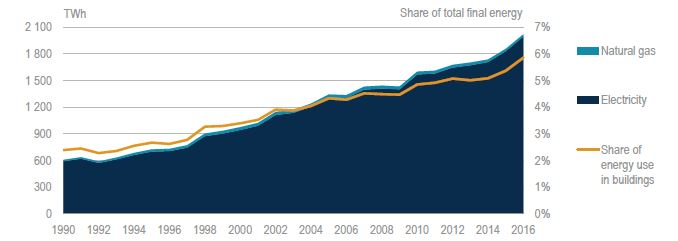
\includegraphics[width=1\textwidth]{cooling_energy.JPG}
	\caption{World energy consumption for space cooling in buildings. Source:\cite{birolFutureCooling2018}}
	\label{fig:cooling_energy}
\end{figure}

A study shows that also in Switzerland cooling demand will strongly increase in the next decades, due to climate change. Figure~\ref{fig:climat_CH} shows how this is particularly true for modern houses, which are very well insulated and efficient for the winter use. In this case the cooling demand will represent more or less a third of the heating demand~\cite{hsluClimaBauPlanenAngesichts2017}.\\

\begin{figure}[h!]
	\centering
	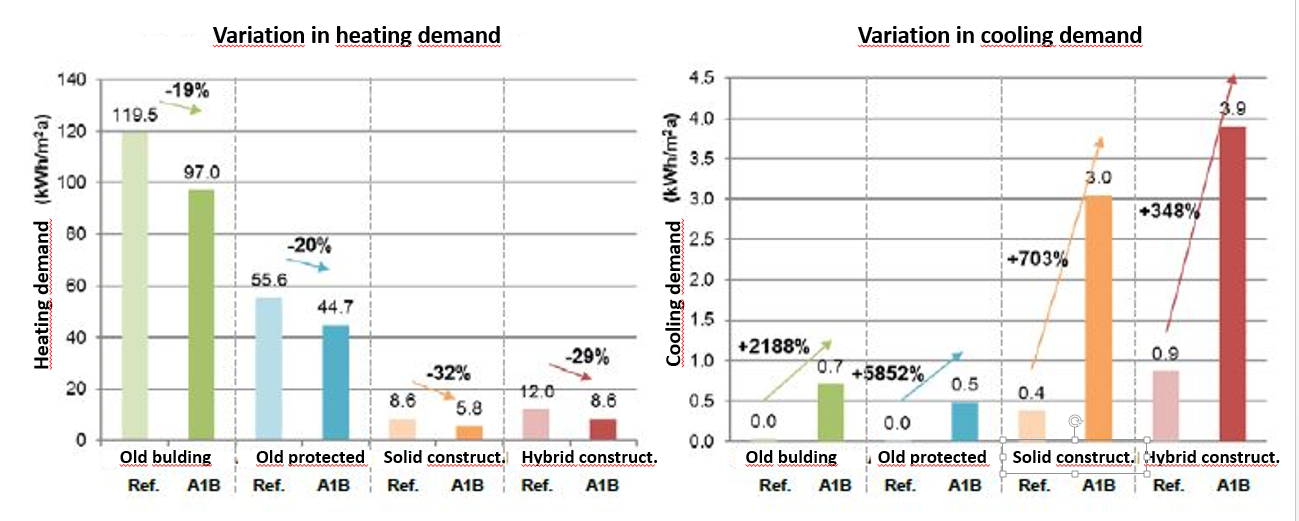
\includegraphics[width=1\textwidth]{clima_CH.jpg}
	\caption{The evolution of median values of heating (left) and cooling (right) demand of the fours case studies ("Old building", "Old builing protected", "Solid construction", "Hybrid construction") between the reference period "1995" (1980-2009) and the period "2060" (2045-2074) in Basel. The percentage variations can be attributed to climate change. A1B corresponds to a median scenario developed by the IPCC. Source:~\cite{hsluClimaBauPlanenAngesichts2017}}
	\label{fig:climat_CH}
\end{figure}

According to the Population Division of the United Nations, the share of the world population living in cities has steadily increased from 34\% in 1960 to 55\% in 2017. Moreover, they prospect that, by 2050, this number will rise to 66\%. In Switzerland, as well as in its neighbouring countries, the percentage of urban population is considerably higher, with 74\% (2017)~\cite{unitednationspopulationdivisionWorldUrbanizationProspects}.
The fact that people live more and more in concentrated areas, also means that the density of energy consumption is rising. This becomes particularly interesting for urban heating and cooling demand, since the high density of heat consumers sets the conditions for efficient  systems, based on district energy networks. 

The UNEP (United Nations Environment Programme) has identified a big potential in modern district energy systems, as the most effective approach to improve energy efficiency for heating and cooling, and enable the integration of renewable energies. However, these technologies require a high level of technology coordination and planning, since they create more efficient systems that are also more complex to deploy and operate. This is why, further research and technology development are needed in order to foster the spreading of these technologies.


\subsection{Scope}
The scope of this project is to pursue the study of the application of the CO2 based district energy network technology, proposed by Weber and Favrat~\cite{weberConventionalAdvancedCO22010}. In collaboration with Romande Energie, the utility company of canton Vaud, a feasibility study was performed on a specific case study: the residential district Eglantine in Morges. The work tried to answer the main research questions:\\
%developed at the Industrial Process and Energy Systems Engineering (IPESE) group at the École Polytechnique Fédérale de Lausanne (EPFL)

\textit{How does the CO2 district energy network perform - ecologically as well as financially - in the Eglantine district, and under which conditions does it perform better than concurrent solutions?}\\

\textit{What are the characteristics of a typical district that favor the choice of the CO2 district energy network technology?}

\newpage
\section{State of the art}

\subsection{District heating}
The evolution of district heating (DH) is shown in Figure~\ref{fig:4GDH}.
The first District Heatings (DH) have been installed in the 1880s in the USA, using concrete ducts to distribute steam at high temperature, which was then condensated by the consumers. This system was obviously not very efficient, due to the elevated heat losses during transportation, as well as the exergy losses due to the high temperature level. In the early 1930 a second generation was developed, which was based on the use of pressurized water, distributed above 100\si{\celsius}. These networks were installed with the purpose of reducing fuel consumption, as well as to integrate the energy generation through CHPs (Combined Heat and Power). The third generation was introduced in the 1980s and it's main difference was the use of a lower distribution temperature (below 100 \si{\celsius}). In those years the main reasons for the installation of DH was security of supply, since they allowed to replace oil with more local and cheaper fuels such as coal, biomass and waste. Moreover, it allowed to use industrial waste heat, as an energy source. 

Nevertheless, a distribution temperature between 70-100 \si{\celsius} still origins very high heat losses, and it does not allow to integrate a larger number of heat sources. Moreover, also in space heating systems in buildings, there has been an evolution towards lower operating temperatures, reducing the average demand temperature. These were the drivers for the development of the $4^{th}$ generation, for which networks operate at a temperature between 30-70 \si{\celsius}. This enables a much better integration of the heating system into the global energy system, as it makes it possible to include low temperature sources (geothermal, solar thermal, refrigeration systems or waste heat from data centers).

\begin{figure}[h!]
\centering
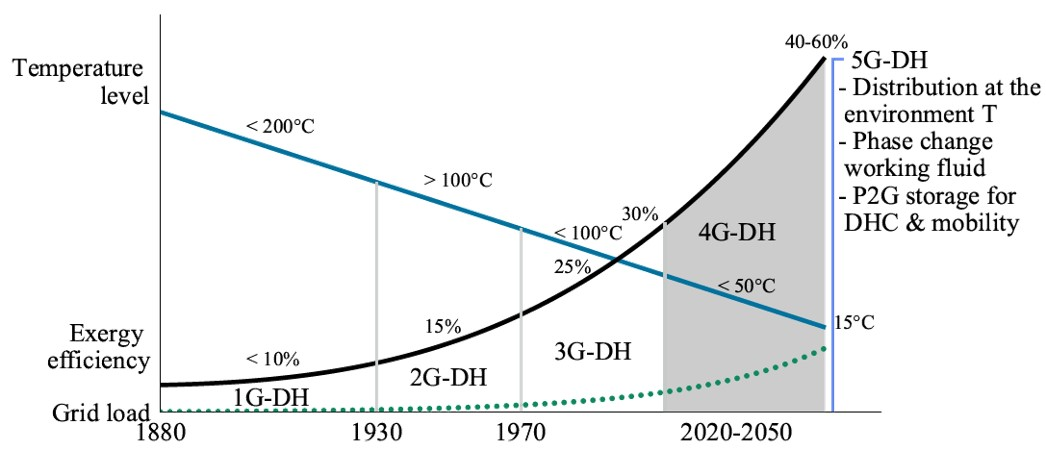
\includegraphics[width=1\textwidth]{5GDH.jpg}
\caption{The evolution of the district heating technology. Source:\cite{lucgirardin5thGenerationDHC2018}}
\label{fig:4GDH}
\end{figure}

\subsection{Fifth generation district energy networks}\label{ss:5gden}
The 4th generation of DH technology, has already achieved remarkable success and has been widely applied, especially in Europe. However, the exergy losses of the system are still very high, due to the diversity of heat levels present in the system, limiting its efficiency. Moreover, the integration of DC, which will become more and more important throughout the next decades, needs the installation of a second and separate networks, which leads to high upfront costs. 

This has lead to the birth of a new technology that uses an even lower distribution temperature (10-25 \si{\celsius}) to provide heating and cooling. In fact, the transfer fluid acts as cold network for cooling purposes and supplies, at the same time, evaporator heat to decentralized heat pumps. This is what is known as the 5th generation DH networks, also known as District Energy Networks (DEN) or District Heating and Cooling (DHC). Besides the higher energy and exergy efficiency, which reduce the operating costs, this technology also reduces the upfront costs. Given the lower distribution temperature, in fact, the pipes require less insulation, as well as they can be placed in shallower depth in the ground.\\

This technology has appeared in Switzerland in 2007, and it's mostly known as \textit{anergy network}, or in german \textit{Anergienetz}. To the authors knowledge, there are seven such systems operating by the end of the year 2018~\cite{energieschweizFallbeispieleThermischeNetze2018}. A summary of a selection of four of them is shown in Table~\ref{tab:anergieCH_sum}, while more detailed information can be found in the Appendix~\ref{as:anergy_suisse}~\cite{energieschweizFallbeispieleThermischeNetze2018}.\\

\begin{table}[h]
\centering
\caption{District energy systems in Switzerland}\vspace{2mm} 
\label{tab:anergieCH_sum} 
\begin{tabular}{llllllll}
\toprule
                                                                                      & \textbf{\begin{tabular}[c]{@{}l@{}}
                                                                                      	Anergienetz \\
                                                                                      	    ETH     \\
                                                                                      	Hönggerberg
                                                                                      \end{tabular}} & \textbf{\begin{tabular}[c]{@{}l@{}}Suurstoffi-\\ Areal\end{tabular}}                             & \textbf{\begin{tabular}[c]{@{}l@{}}Anergienetz \\ Friesenberg (FGZ)\end{tabular}} & \textbf{\begin{tabular}[c]{@{}l@{}}Genève-Lac-\\ Nations (GLN)\end{tabular}} \\
\midrule
\textbf{Location}                                                                     & Zürich                                                                             & Rotkreuz                                                                                         & Zürich                                                                            & Genève                                                                       \\
\textbf{Year of construction}                                                         & 2012 - 2026                                                                        & 2010 - 2020                                                                                      & 2011-2050                                                                         & 2008 - 2016                                                                  \\
\textbf{ERA [m2]}                                                                     & 475'000                                                                            & 172'421                                                                                          & 185'000                                                                           & 840'000                                                                      \\
\textbf{\begin{tabular}[c]{@{}l@{}}Inst. Heating\\ capacity [kW]\end{tabular}}        & 8'000                                                                              & 6'732                                                                                            & 3'930                                                                             & 4'300                                                                        \\
\textbf{\begin{tabular}[c]{@{}l@{}}Heating demand \\ '[MWh/a]'\end{tabular}}          & 28'450                                                                             & 10'619                                                                                           & 35'000                                                                            & 5’000                                                                        \\
\textbf{\begin{tabular}[c]{@{}l@{}}Inst. Cooling\\ capacity [kW]\end{tabular}}        & 6'000                                                                              & 2'327                                                                                            & 3'500                                                                             & 16'200                                                                       \\
\textbf{\begin{tabular}[c]{@{}l@{}}Cooling demand \\ '[MWh/a]'\end{tabular}}          & 26'200                                                                             & 2'364                                                                                            & 80'000                                                                            & 20'000                                                                       \\
\textbf{Distribution fluid}        & water                                                                              & water                                                                                            & water                                                                            & water                                                                       \\
\textbf{Heat source}                                                                  & \begin{tabular}[c]{@{}l@{}}Laboratories\\ waste heat \\ +HP\end{tabular}           & \begin{tabular}[c]{@{}l@{}}Waste heat \\ buildings \\ + PVT (solar th.) \\ +HP\end{tabular}      & \begin{tabular}[c]{@{}l@{}}Waste heat\\ data center+HP\end{tabular}               & Lake water +HP                                                               \\
\textbf{Heat storage}                                                                 & \begin{tabular}[c]{@{}l@{}}Geothermal well \\ field\\ (431 at 200m)\end{tabular}   & \begin{tabular}[c]{@{}l@{}}Geothermal well\\ field \\ (215 at 150 m,\\ 180 at 280m)\end{tabular} & \begin{tabular}[c]{@{}l@{}}Geothermal well\\ field\\ (332 at 250m)\end{tabular}   & None                                                                         \\
\textbf{T of heating pipe}                                                                & 24 \si{\celsius} - 8 \si{\celsius}                                                                       & 25 \si{\celsius} - 8 \si{\celsius}                                                                                     & 28 \si{\celsius} - 8 \si{\celsius}                                                                      & 17 \si{\celsius} - 5 \si{\celsius}                                                                 \\
\textbf{T of cooling pipe}                                                                & 4 \si{\celsius} - 20 \si{\celsius}                                                                       & 4 \si{\celsius} - 17 \si{\celsius}                                                                                     & 4 \si{\celsius} -24 \si{\celsius}                                                                       & 5 \si{\celsius} - 12 \si{\celsius}                                                                 \\
\textbf{\begin{tabular}[c]{@{}l@{}}Tot. investments\\ '[Mio.CHF]'\end{tabular}}       & 37                                                                                 & n/a                                                                                              & 42.5                                                                              & 33                                                                           \\
\textbf{\begin{tabular}[c]{@{}l@{}}
	Tot. COP of heating \\
	  (incl. Pumps…)
\end{tabular}} & 5.8                                                                                & 2.7                                                                                              & 4.1                                                                               & 6.5                                                                            \\
\bottomrule
\end{tabular}
\end{table}


All the anergy networks presented in Table~\ref{tab:anergieCH_sum} still base on water as a working fluid. Therefore, they work on sensible heat, which means that a heat exchange is bound to a variation in the fluids temperature. The challenge of these systems is given by the flow rate that is necessary to limit the temperature difference between the inlet and the return temperature of the network. Thus, it could be very interesting to use refrigerants, instead of water, that enable to work with latent heat instead, which means collecting and distributing heat through the condensation, or the evaporation, of the refrigerant. This poses some additional technological challenges, but has also very clear advantages, as it will be shown in the next chapters.\\

\begin{figure}[h!]
	\centering
	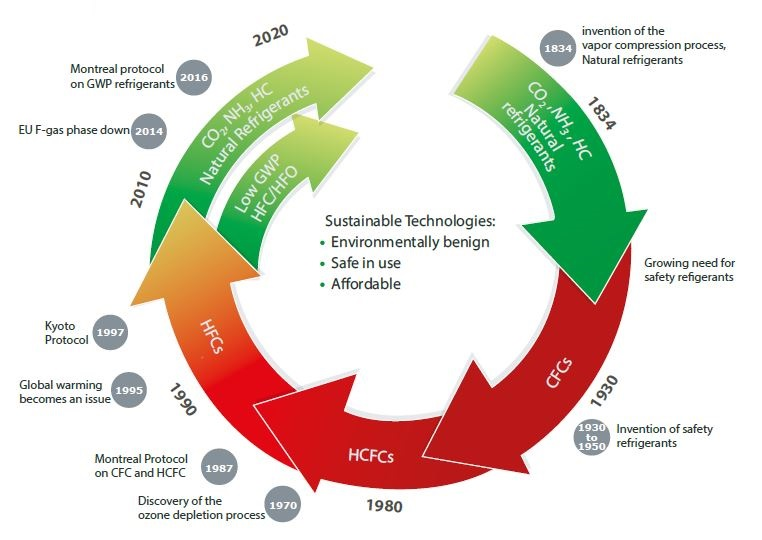
\includegraphics[width=0.7\textwidth]{refrigerants.JPG}
	\caption{The historical cycle of refrigerants Source:~\cite{danfossRefrigerantOptionsNow2017}}
	\label{fig:refrigerants}
\end{figure}

The choice of the refrigerant strongly depends on the application. In function of the operating conditions, three main criteria are evaluated: affordability, safety and environmental impact.
A summary of the history of refrigerants is shown in Figure~\ref{fig:refrigerants}.
The Montreal protocol, signed in 1987, designed the phase out of HCFC and CFCs, in order to prevent ozone layer depletion. This boosted the use of HFCs, as a replacement. However, not far later, it has been realized that despite being less damaging to the ozone layer, they were powerful greenhouse gases. Since 2013, a federal ordinance also strongly restricted the use of these last ones in Switzerland~\cite{hydrocarbons21.comSwitzerlandIntroduceHFC}. Also Europe planned the phase-out of HFC in 2014~\cite{europeancommissionforclimateactionEULegislationControl2016}. This means that today the choice of refrigerants is essentially limited to natural refrigerants - as for example CO2 (R744), ammonia (R717) or propane (R290) - and the new environmentally friendly HFOs - as for example the fluorinated propane isomer R1234yf.\\

The choice of CO2 as a refrigerant relies, besides its thermodynamic properties, on the following arguments~\cite{cavalliniPropertiesCO2Refrigerant2004}:
\begin{itemize}
	\item it is very abundant in the environment and is also waste of a multitude of industrial processes
	\item it is harmless to the biosphere
	\item it is non-flammable and non-toxic
	\item it is an inert gas
\end{itemize}

In fact, according to Danfoss~\cite{danfossRefrigerantOptionsNow2017}, CO2 will dominate industrial refrigeration, together with ammonia. Already today, this technology is widely used. For instance Migros, Switzerland's largest retail company, opened its first supermarket to use CO2, in a low-temperature subcritical system, in 2002. By today, 411 of the 700 supermarkets in Migros’s portfolio are equipped with transcritical CO2 systems~\cite{williamsMigrosDNA2018}.


\subsection{CO2 district energy network}

%Generally, however, refrigerant based DEN are still at a prototype stage.

\subsubsection{The technology}
Weber and Favrat~\cite{weberConventionalAdvancedCO22010} compared the performance of a DEN using subcritical CO2, HFO R1234yf and water. They were able to show that the CO2 network performs best, and has the biggest potential for DEN systems~\cite{henchozPotentialRefrigerantBased2016}. 
As explained above, a refrigerant based DEN technology allows to store and transfer heat through the latent heat of vaporization of the refrigerant. The operating pressure is chosen in order to obtain the desired temperature in the system. That temperature is selected to be as high as possible to represent a good heat source for the decentralized heating heat pumps - resulting in good COP values -, while still allowing free cooling - avoiding the installation of compression chillers, and thus drastically reduce electricity consumption for space cooling. 

The network consists of one saturated liquid pipe and of one saturated vapor pipe, both in a saturated temperature range from 12 to 18 \si{\celsius}~\cite{suciuEnergyIntegrationCO22018}.
The working principle is shown in Figure~\ref{fig:CO2schema}. Heating users can extract heat from the network through condensation of the refrigerant, taken from the vapour pipe. Respectively, cooling users take refrigerant from the liquid pipe and evacuate heat by evaporating it. The heat exchanges between the network and the users occur through condenser-evaporators heat exchangers, which keep the different refrigerant loops isolated~\cite{henchozPotentialRefrigerantBased2016}. The synergy between simultaneous heating and cooling users allows the recovery of waste heat. Most of the time, the required heating and cooling capacity will not be equal, which means that there is the need for a centralized balancing power. Indeed, a central plant is responsible to balance the overall network, by exchanging heat with the environment. For instance, a ground/water or a water/water heat pump can be used for this purpose.\\

%A comparison of the energy performance of two refrigerant based networks, CO2 and HFO R1234yf, and one cold water
%(anergy) network can be found in Ref.:
%S. Henchoz, P. Chatelan, F. Maréchal, and D. Favrat, “Key energy and technological
%aspects of three innovative concepts of district energy networks,” in Proceedings Of
%the 28th International Conference On Efficiency, Cost, Optimization

\begin{figure}[h!]
\centering
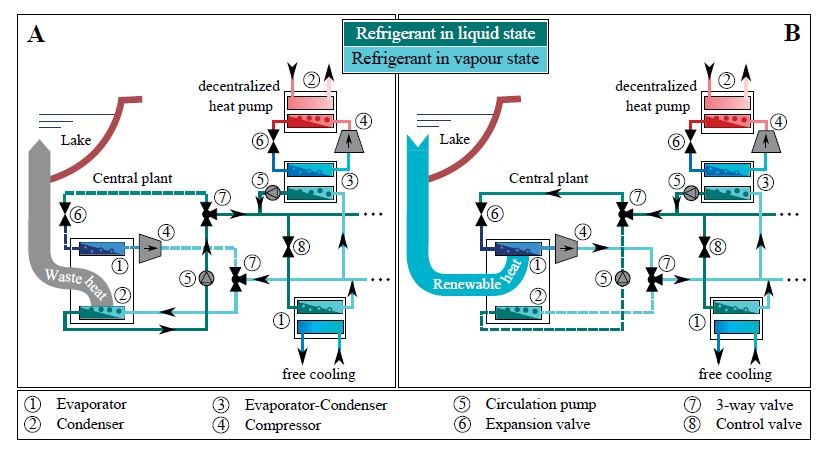
\includegraphics[width=1\textwidth]{CO2schema.JPG}
\caption{Schematics of a refrigerant based district energy network. Part A represents its net cooling operation, and part B its net heating operation. Source:~\cite{henchozPotentialRefrigerantBased2016}}
\label{fig:CO2schema}
\end{figure}

One of the big advantages of this technology, with respect to water based DEN, is the pipes sizing. In fact, given the fact that it works on pressure maintenance instead of a fluid flow, no return pipe is necessary, which results in a slightly shorter total length of installed pipes. Moreover, due to the higher energy density of latent heat, the pipes diameters are drastically reduced. Henchoz et al.~\cite{henchozPotentialRefrigerantBased2016} compared three different working fluid on the same study case, showing that, while CO2 needs pipes of only 280/330mm (liquid/vapor), R123yf would need 270/700mm (liquid/vapor) and water 625/625mm (liquid/liquid). Given the low operating temperatures, there are much lower requirements for pipes insulation. While water pipes need to be buried deep enough to prevent damage due to water freezing, in case part of the network had to be stopped during winter, CO2 does not freeze and thus does not require a minimum freeze-safe depth. Henchoz et al. have even imagined installing the pipes inside a sidewalk module, which would drastically simplify maintenance and inspection. Given the smaller diameter, it would also be possible to retrofit an old, high temperature district heating network, by placing the CO2 pipes inside the old water pipes. All the above mentioned advantages of using CO2, result in lower upfront costs. \\

The main drawback of this technology is the high operating pressure - about 50 bars - and the safety concerns that could derive from the large amount of CO2 that could escape in case of a major leakage. Nevertheless, as described in~\ref{ss:5gden}, CO2 refrigeration networks are already widely used in supermakets, and the technology is considered as safe. \\

%\textit{Safety issues analyzed~\cite{girardinSafetyIssuesCO2based2016}.\\}
%\textit{A cold water network is the second best option, although more expensive initially and thus less profitable, it has several advantages in terms of safety and availability of components.}

\subsubsection{Performance}
Henchoz et al.\cite{henchozPotentialRefrigerantBased2016} performed an analysis of the potential application of a CO2 based DEN in a district in the city of Geneva. A map of the district, called "Rues basses", is shown in Figure~\ref{fig:henchoz_gva}.

\begin{figure}[!htb]
	\centering
	\begin{minipage}{.45\textwidth}
		\centering
		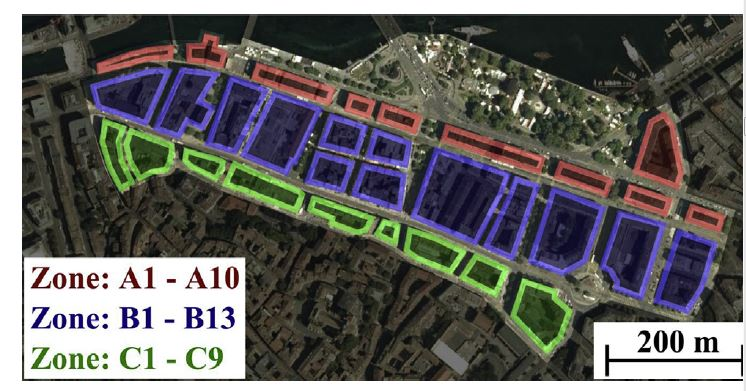
\includegraphics[width=\textwidth,height=0.2\textheight]{henchoz_gva.JPG}
		\caption{Representation of the the studied area and of its subdivision into 32 zones. Source:~\cite{henchozPotentialRefrigerantBased2016}}
		\label{fig:henchoz_gva}
	\end{minipage}%
\hspace{1cm}
	\begin{minipage}{0.45\textwidth}
		\centering
		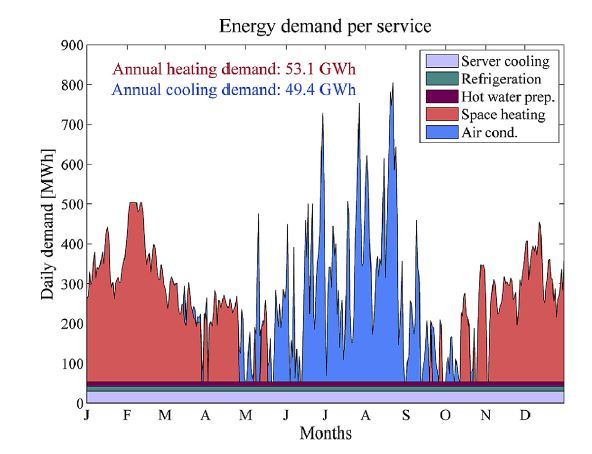
\includegraphics[width=\textwidth,height=0.2\textheight]{henchoz_energydemand.JPG}
		\caption{Energy demand for the area studied over the year 2012. Source:~\cite{henchozPotentialRefrigerantBased2016}}
		\label{fig:henchoz_energydemand}
	\end{minipage}
\end{figure}


%\begin{figure}[h!]
%\centering
%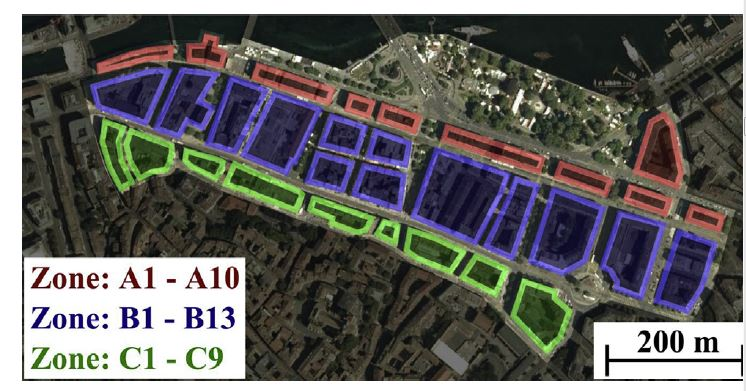
\includegraphics[width=0.5\textwidth]{henchoz_gva.JPG}
%\caption{Representation of the the studied area and of its subdivision into 32 zones. Source:~\cite{henchozPotentialRefrigerantBased}}
%\label{fig:henchoz_gva}
%\end{figure}

Table~\ref{tab:henchoz_area} shows the distribution of building affectations - which is important to determine the energy consumption - in the studied area. The total ERA is $687'800 \ m^{2}$.\\

\begin{table}[h!]
\centering
\caption{Distribution of the energy reference area for the different zones and building affectations}\vspace{2mm}
\label{tab:henchoz_area} 
\begin{tabular}{llll}
	\toprule
	Zones          & Commercial [$m^{2}$ ERA] & Offices  [$m^{2}$ ERA] & Residential  [$m^{2}$ ERA] \\ \midrule
	A1 - A10       & 20'700                   & 89'200                 & 17'700                     \\
	B1 - B13       & 97'000                   & 260'700                & 61'600                     \\
	C1 - C9        & 40'400                   & 62'600                 & 48'100                     \\ \midrule
	Relative share & 23\%                     & 60\%                   & 17\%                       \\ \bottomrule
\end{tabular}
\end{table}

The energy demand of heating ($53.1 GWh/yr$) and cooling ($49.4 GWh/yr$) in the studied area is shown in Figure~\ref{fig:henchoz_energydemand}. Throughout the year, the district presents nearly the same heating demand as for cooling, but they happen in different seasons. 

%\begin{figure}[h!]
%\centering
%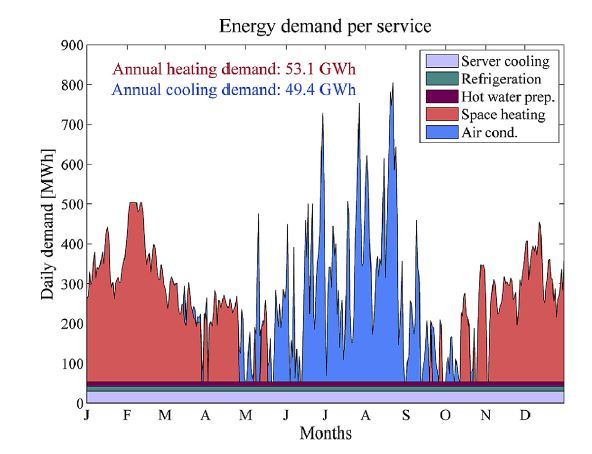
\includegraphics[width=0.75\textwidth]{henchoz_energydemand.JPG}
%\caption{Energy demand for the area studied over the year 2012. Source:~\cite{henchozPotentialRefrigerantBased}}
%\label{fig:henchoz_energydemand}
%\end{figure}

The proposed CO2 based DEN is balanced by a central plant - a heat pump - that exchanges heat with the nearby lake. In order to benchmark the results, this technology has been compared to a traditional heating and cooling system, based on oil boilers and cooled compression chillers.

The results are remarkable. In fact, the CO2 based DEN shows a final energy consumption of 10,968 MWh of electricity, which corresponds to a reduction of 84.4 \%, with respect to the reference scenario. Its exergy efficiency situates between 40-45\%.
%
%\todo{CO2gva: Talk about financial numbers comparison? Otherwise delete fig~\ref{fig:henchoz_costs}}
%
%\begin{figure}[h!]
%\centering
%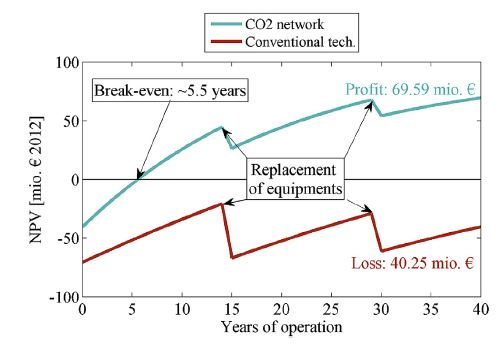
\includegraphics[width=0.5\textwidth]{henchoz_costs.JPG}
%\caption{Evolution of the net present value over the lifetime of the two energy conversion technologies. Source:~\cite{henchozPotentialRefrigerantBased}}
%\label{fig:henchoz_costs}
%\end{figure}


\subsubsection{Integration in smart energy system}
The integration of high shares of renewable energy represents an important challenge. In fact, it requires a lot of slack to handle the volatile nature of renewable energy sources like wind or sun. On one side, this slack will be mainly given through a smart control of the electricity grid on multiple levels. It starts from the demand side management (DSM) inside households, through optimization at district level, up to a national and international control. These decentralized grids, or grid controls, are called \textit{smart grids}. \\

With the vast success of heat pumps throughout the last decade, the control of electricity grids is more and more interconnected with the production of heat. This further complexifies the system by adding a level of constraints, but it also opens new levels of control. Indeed, if well designed, a DEN offers an additional level of slack that can be used in combination with the smart grid, multiplying control power. The CO2 DEN offers several possibilities to shift the loads, relieving the grid. \\

On the one hand, it simplifies the deployment of a smart control of the heat pumps, which can strongly contribute in the DSM. The decentralized heat pumps can make use of a buildings thermal inertia to adapt electricity use to energy availability. CO2 vapor and liquid storage can act as a buffer, enabling load-shifting also for the central plant of the DEN. Sizing of these storage capacities will determine the possible time-span that the shift can achieve. Given the low distribution temperature, this approach also facilitates the storing of heat, as for example in a geothermal field.

On the other hand, the use of CO2 as a refrigerant for the network could improve the integration of a power to gas (PtG) system. Indeed, one big challenge in the future, especially in higher latitudes, where seasonal variation are consistent, is to ensure energy supply during winter season, when, due to shorter and weaker solar irradiation, PV panels produce less. It is thus important to find a way to store the excess of renewable energy production during the summer, in order to use it in the winter.
One solution to do that is PtG, which defines the process of transforming electrical power to a gas, like methane, which is easy to store. To do so, electricity is used to produce hydrogen, which can be combined with CO2 to form Methane, in a process called methanation. Methane can be used during winter to produce electricity and heat, in a combined heat and power plant (CHP), as for example a SOFC, a gas turbine, or a combination of them. For this reason, PtG is widely studied across Europe and many pilot plants have already been built~\cite{ProjectsEuropeEuropean}.\\ 
Suciu et al.~\cite{suciuEnergyIntegrationCO22018} studied the synergy between a CO2 based DEN, decentralized PV and such a PtG system. The CO2 network could be used to store the carbon dioxide, which is captured from CHPs or industrial processes during winter, needed for methanization. At the same time, the DEN can directly use and dispatch the heat produced from the CHPs. In their work, they analyzed the PV area, and thus the investment, required to achieve a completely autonomous energy system, for different European climatic zones. The results showed that decarbonized autonomous energy systems based on DENs and PtG tecnologies are possible, along with a very broad deployment of solar energy. It is also shown that the payback time of such a system is between 11 and 14 years, which is relatively low compared to its life time.

\subsection{Direct-expansion ground source heat pump}\label{ss:dx}

For heat pumps based systems, sourcing heat from the soil, instead of from the ambient air, is a very interesting solution at central European latitudes, especially, as it has been seen, for integration of a 5th generation DEN, since it improves heating and cooling COPs, and, to a certain extent, it allows heat storage. In traditional Ground-Source Heat Pumps (GSHP), the heat pump and the ground are connected by means of a closed loop, using water, or a water solution. This system, called the secondary loop GSHP (SL-GSHP), is shown on the right side of Figure~\ref{fig:gshp}. However, it has been proved~\cite{kruseStatusDevelopmentResearch2010, guoTechnoeconomicComparisonDirect2012} that the system efficiency can be improved, by directly expanding the refrigerant into the ground, avoiding the secondary water loop. Shown on the left side of Figure~\ref{fig:gshp}, this system is called Direct Expansion GSHP (DX-GSHP). 

\begin{figure}[htp]
\centering
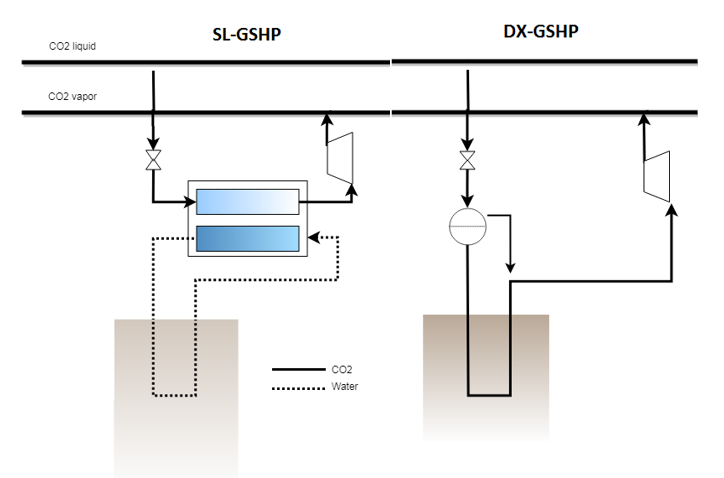
\includegraphics[width=0.8\textwidth]{CO2-DX}
\caption{A simplified schematics of the two GSHP technologies}
\label{fig:gshp}
\end{figure}

So far, this technology is not so widely spread, mostly because of a more demanding system design and because of the risk of environmental pollution, when non-natural refrigerants are used. Indeed, literature about DX-GSHP is still scarce, especially for CO2 as a refrigerant. The are only few numerical CO2-DX-GSHP studies~\cite{eslami-nejadModelingTwophaseCO2filled2014,ghazizade-ahsaeeEnergyExergyInvestigation2018,austinParametricStudyPerformance2011,eslami-nejadQuasitransientModelTranscritical2015}, which are not yet sufficient to obtain a scientific appreciation of the technology. Nevertheless several prototypes and experimental set-ups have been built and analyzed~\cite{eslami-nejadDetailedTheoreticalCharacterization2018, badacheExperimentalStudyCarbon2018, guoTechnoeconomicComparisonDirect2012}, showing that higher efficiencies can be reached through DX, with respect to a SL.

On of the main reasons for this efficiency gain is the elimination of the temperature lift of the water loop, which is replaced by a constant temperature phase-change, as well as the elimination of the minimum approach temperature necessary to exchange heat between the SL and the heat pump, as shown in Figure~\ref{fig:Qt_dx}. The resulting temperature rise for the DX-GSHP $\Delta T_{HP}^{DX}$ is much lower than $\Delta T_{HP}^{SL}$ for the SL-GSHP, leads to a higher COP for the heat pump. 
Moreover, CO2 presents a higher heat transfer coefficient, which again allows to either reduce the minimum approach temperature, or extract a higher power with respect to an equal exchange surface. The minimum approach temperature has to be determined in function of the thermal permeability of soil and is correlated to the length and total surface of the geothermal probes, as well as the refrigerant flow rate.

\begin{figure}[htp]
	\centering
	\includegraphics[width=0.8\textwidth]{Qt_dx.png}
	\caption{Schematic representation of heat exchanges and minimum approach temperatures for the central plant HP, comparing SL- and DX-GSHP}
	\label{fig:Qt_dx}
\end{figure}

\clearpage
\newpage
\section{Methodology}

\subsection{Energy demand - Typical days}\label{ss:typicalDays}
The energy demand profile for space heating and cooling is calculated as a a linear function of the temperature difference with the ambient temperature~\cite{girardinEnerGisGeographicalInformation2010}. Specific energy requirements per square meter in function of the typology of the building are taken from SIA (Schweizerischer Ingenieur- und Architektenverein) standards~\cite{siaSIA38020162016}.\\

The optimization of an energy system is commonly performed over the time span of one year, in order to account for the different seasons. However, this requires a very long computing time, given the high number of time steps. Thus, it is common to group similar days, according to a set of parameters as for example temperature or irradiation, into so called typical days. The days can be clustered in different ways. It can be chosen to compute an average day for each month or some machine learning clustering algorithm - as for example K-means, DBSCAN or GMM - can be used to group the days into the desired number of clusters.
The resulting typical days correspond to a period $p$, with a number of times $t$, as explained in section~\ref{ss:osmose}. In order to account for the data compression, a value called $occurrence$ indicates how many times a given typical day occurs, i.e. how many times a given period occurs.

Two additional days with the two opposite extreme temperature conditions are added to the typical days, in order for the model to account for them in the equipment sizing. To avoid a bias of the operation results, those days are set with an occurrence of zero.


\subsection{Geothermal wells}\label{ss:gtw}

The most important parameter in geothermal wells is the soil temperature, which is normally constant throughout the year. In fact, only the first 10 meters are influenced by the temperature of the air~\cite{hanSensitivityAnalysisVertical2016}. Moreover, the temperature increases with depth. According to the SIA norm SIA384~\cite{siaSIA384Sondes2010}, the mean temperature in a geothermal well can be calculated by:
\begin{equation}
T_{g, mean} = T_{g,sup} + \frac{L_{w} \cdot \nabla T_{g}}{2}
\end{equation}
where $T_{g,sup}$ is the ground temperature at the surface, $L_{w}$ is the length of the well and $ \nabla T_{g}$ is the temperature gradient of the soil. 

The energy demand of the circulating pumps is assumed to be negligible. 

\subsection{Investment cost function}\label{ss:ic}
To calculate the investment cost for a given technology, it is possible to interpolate data from available products on the market. However, it is also possible to evaluate it with help of a cost function~\cite{turtonrichardc.bailierichardwhitingwallace.AnalysisSynthesisDesign2003}.

First, it is necessary to calculate the cost of purchase of the unit, in function of its size, given by the sizing parameter, which can be the electrical power $E$, the delivered heat $Q$ or the area of a heat exchanger $A$.

\begin{equation}
C_{pex} = \frac{I_{t}}{I_{t,ref}} \cdot 10^ {(k_{1,ex} + k_{2,ex} \cdot \log(E/Q/A))}
\end{equation}

Through a factor called \emph{Bare Module Factor}, the accessory costs of transport, installation, connection are included in the calculation, obtaining the total investment costs

\begin{equation}
CBM_{ex} = C_{pex} \cdot FBM_{ex} \cdot e 
\end{equation}

where $e$ is the currency ration from USD to CHF. The annuities are calculated with the annualization factor ($af$), where $n$ is the assumed lifetime of the equipment in years, and $i$ the interest rate. 

\begin{align}
	& IC_{yearly,ex} = CBM_{ex} \cdot af 
	& af = \frac{i \cdot (1 + i)^n}{(1 + i)^n - 1}
\end{align}

This investment cost function is not a linear function. However, as described in Section~\ref{ss:osmose}, to solve the MILP it is necessary to provide a set of linear parameters that approximate the function. These are found by linearizing the investment cost function around the reference value, defined in the range of application. This was done with help of a matlab code, using \textit{polyfit} and \textit{polyval} functions. Figure~\ref{fig:lin} shows the linearized function with the according cost parameters.

\begin{figure}[htp]
	\centering
	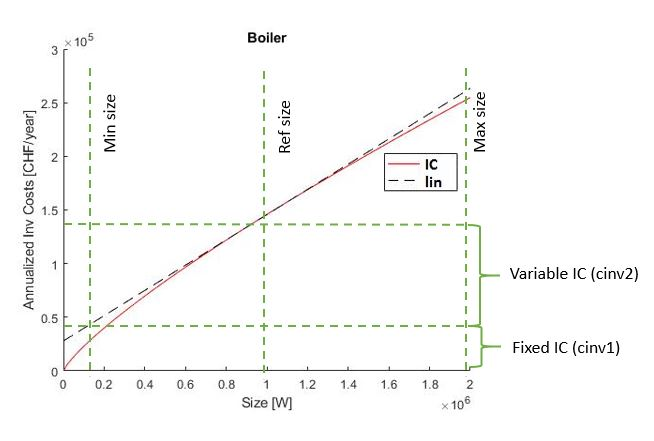
\includegraphics[scale=0.6]{Images/linearization_expl.jpg}
	\caption{Linearization of investment cost function}
	\label{fig:lin}
\end{figure}

\subsection{Minimum approach temperature}\label{ss:dtmin}
The critical sizing parameter for a heat exchange is the minimum approach temperature $\Delta T_{min}$, which corresponds to the smallest temperature difference in the heat exchanger between the hot and the cold stream, as shown in Figure~\ref{fig:dtmin}. This value is strongly dependent on the heat exchanger area $A_{ex}$ and the heat transfer coefficients $h$ of the exchanging fluids. 

\begin{equation}\label{eq:HEX_area}
A_{ex} = \frac{Q_{ex}}{U \cdot LMTD}
\end{equation}
\begin{equation}\label{eq:LMTD}
LMTD= \frac{(T_{Hot,in } - T_{cold,out }) - (T_{Hot,out } - T_{cold,in }) }{ \log{ (\frac{T_{Hot,in } - T_{cold,out }}{T_{Hot,out } - T_{cold,in }} ) }}
\end{equation}
\begin{equation}
	T_{Hot,in } = T_{cold,out} + \Delta T_{min}
\end{equation}
where  $LMTD$ is the logarithmic mean temperature difference and T are the inlet and outlet temperatures of the hot and cold streams, as shown in Figure~\ref{fig:dtmin}. The overall heat transfer coefficient~\cite{huExtremumSeekingControl2015} is given by:
\begin{equation}\label{eq:alpha}
U= \frac{1}{ \frac{1}{h_{(hot)} } + \frac{1}{h_{(cold)}} }
\end{equation}
where $h_{(hot)}$ and $h_{(cold)}$ are the heat transfer coefficient of the hot and cold fluid.

\begin{figure}[htp]
	\centering
	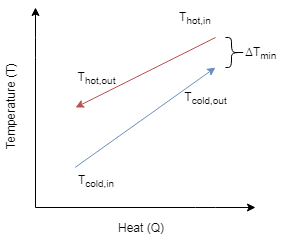
\includegraphics[scale=0.5]{Images/dtmin.png}
	\caption{Minimum approach temperature in a counter-flow heat exchanger.}
	\label{fig:dtmin}
\end{figure}

The optimization is done by minimizing the total cost of the system dependent on the heat exchange, which include the investment and operating costs of the compressor, as well as the investment costs of the heat exchanger:
\begin{equation}
	\min_{\Delta T_{min}}\left\lbrace OC(\Delta T_{min}) + IC(\Delta T_{min}) \right\rbrace 
\end{equation}

A bigger $A_{ex}$ allows a smaller $\Delta T_{min}$, which increases the investment costs of the heat exchanger. However, a smaller $\Delta T_{min}$ also reduces the temperature difference that the heat pump has to achieve in order to exchange heat, thus increasing its COP. This leads to a lower electricity consumption, i.e. lower operating costs, as well as to a lower investment cost of the compressor. An optimum can be found for each specific application.\\

Heat transfer coefficients used in this work are shown in Table~\ref{tab:alphas}. For R134yf, the heat transfer coefficient appears to be the same as for R134a~\cite{wangOverviewHeatTransfer2013}, while for CO2 (R744) experimental values are used~\cite{ohFlowBoilingHeat2011, mastrulloComparisonR744R134a2009}. \\

\begin{table}[h!]
\centering
\caption{Heat transfer coefficients found in literature}\vspace{2mm}
\label{tab:alphas} 
\begin{tabular}{llll}
	\toprule
	Fluid             & Water & R134yf & R744 \\ \midrule
	$h [W/(mK)]$ & 600   & 3000   & 7000 \\ \bottomrule
\end{tabular}
\end{table}


\subsection{Exergy}\label{ss:exergy}
The exergy of an energy transfer is defined as the maximum amount of work that can be extracted from it, through reversible transformations that exchange with the environment. Thus the calculation of exergy losses is a very interesting indicator to analyze a given process or system, since it expresses the quality and the efficiency with which the system operates, with respect to the maximum possible. Therefore these values are always lower than 100 \%. \\

The exergy value is derived from the first two thermodynamic principles, and is given by the following formula~\cite{henchozPotentialRefrigerantBased2016}:
\begin{equation}
    \dot{E}^{-}_{max} = \sum_{i} \dot{Q_i}^{+} (1 - \frac{T_{a}}{T_i} ) + \sum_{r} \dot{M}_{r}^{+} (h_{r} - T_{a} s_{r})    
\end{equation}

The exergy losses are thus given by the difference between the exergy value and the energy furnished to the system:
\begin{align}
	&    \dot{L} = \dot{E}^{-}_{max} - \sum_{j}\dot{E}^{-}_{j} \geq 0 \\
	& 	\dot{L} = (1-\eta_{exergy})\dot{E}^{-}_{max}
\end{align}

In the case of a heat pump based energy system, the exergy is given by:
\begin{align}
    & \eta_{exergy} =  \frac{\dot{E}q_{cold,a} + \dot{E}q_{hot,r}}{\dot{E}_{el}^{+}}  \\
    & \dot{L} = (1-\eta_{exergy})\dot{E}_{el}^{+}
\end{align}
where $\dot{E}q_{hot,r}$  and $\dot{E}q_{cold,a}$ are the exergy value of respectively the hot streams below (r) and the cold streams above (a) the ambient temperature; these correspond to the exergy value of the heating and cooling demand. $\dot{E}_{el}^{+}$ is the electricity consumed by the defined system, which corresponds to the energy furnished to the system in order to satisfy the demand.

\subsection{Energy technology models}\label{ss:et}
The models for the energy technologies are adapted from an existing source code~\cite{suciuEnergyautonomousCitiesUsing2016}, as explained in detail in this chapter.

\subsubsection{Heat pump - Carnot cycle}\label{sss:hp_carnot}
Heat pumps can be modeled in a simple way, using the principle of the Carnot cycle, with help of the following equations:
\begin{align}
    & \dot{E}_{compressor} = \frac{\dot{Q}_{cond}}{COP_{real}} = \frac{\dot{Q}_{cond}}{\eta_{COP} \cdot COP_{theoretical}} \\
    & COP_{theoretical, heating} =  \frac{T_{h}}{T_{h} – T_{c}}  
    & COP_{theoretical, cooling} =  \frac{T_{c}}{T_{h} – T_{c}} 
\end{align}
where $\dot{Q}_{cond}$ is the heat delivered and $\dot{Q}_{evap}$ the heat sourced by the heat pump. $\eta_{COP}$ is an experimentally defined efficiency to account for irreversibility of the cycle, i.e. to give the ratio between the theoretical and the real COP. The values used in this work are shown in Table~\ref{tab:etaCOP}, calculated by Girardin et al.\cite{girardinEnerGisGeographicalInformation2010}, based on values obtained from c heat pump certification center~\cite{NTBBuchsInstitut}. \\

\begin{table}[h!]
\centering
\caption{Theoretical efficiency factor for COP}\vspace{2mm}
\label{tab:etaCOP} 
\begin{tabular}{lll}
	\toprule
	Type         & Size          & $\eta_{COP}$ \\ \midrule
	Air/Water    & Decentralized & 0.34         \\
	CO2/Water    & Decentralized & 0.43         \\
	Ground/Water & Decentralized & 0.43         \\
	Ground/Water & Centralized   & 0.55         \\
	Water/Water  & Centralized   & 0.55        \\ \bottomrule
\end{tabular}
\end{table}


\subsubsection{Heat pump - Thermodynamic cycle}\label{sss:hp_thermo}

\begin{figure}[htp]
	\centering
	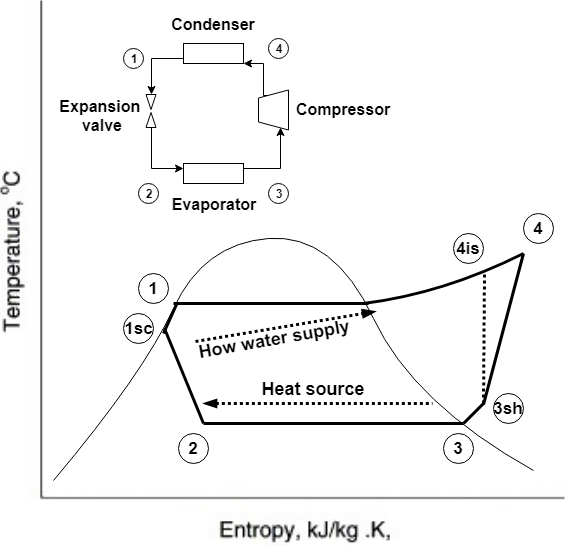
\includegraphics[width=0.5\textwidth]{HP_cylce_ref.png}
	\caption{Temperature–entropy diagram of a R134yf based heat pump system.}
	\label{fig:hp_ref}
\end{figure}

A more accurate model of the heat pumps, that is able to correctly represent and calculate the operating cycles and conditions, is achieved by modeling its thermodynamic cycle~\cite{demierreModelingExperimentalInvestigation2014}, represented in Figure~\ref{fig:hp_ref}:

\begin{description}
	\item [1 - 2]: Expansion to low pressure level
	\item [2 - 3]: Evaporation by cooling down the heat source
	\item [3 - 3sh]: Superheating in evaporator
	\item [3sh - 4]: Compression to high pressure level
	\item [4 - 1]: Condensation of refrigerant, delivering heat
\end{description}

The compressor is a crucial component for the design of a heat pump, since it has the largest share of impact on the energy efficiency. To calculate its efficiency, the model of Hu et al.\cite{huExtremumSeekingControl2015} has been used. The shaft power can be computed in function of the isentropic efficiency ($\eta_{is}$) by:
\begin{equation}
W_{shaft} = \frac{\dot{m}(h_{d,is}-h_{s})}{\eta_{is}} 
\end{equation}
where $h_{d,is}$ is the isentropic discharge enthalpy and $h_{d}$ is the suction enthalpy. The compressors input power is expressed in function of its mechanical efficiency ($\eta_{mech}$) by:
\begin{equation}
E_{comp} = \frac{W_{shaft}}{\eta_{mech}}  
\end{equation}

The numerical values of those efficiencies are strongly dependent on the ratio between the pressure of discharge $P_{d}$ and the pressure of suction $P_{s}$ of the compressor.They can be computed inside the model with help of the relations obtained by Li et al.\cite{liPerformanceCharacteristicsR1234yf2014}:
\begin{align}
& \eta_{mech} = 0.85\\
& \eta_{is} = 0.874-0.0134\cdot(\frac{P_{d}}{P_{s}})\\
\end{align}
		
The expansion of the refrigerant in the expansion valve is assumed to be isenthalpic.\\ 

Thus, the procedure to evaluate the operating conditions of the heat pump is the following:
\begin{enumerate}
	\item calculate thermodynamic state in point (1) knowing the evaporation temperature $T_{evap}$ and assuming saturated liquid
	\item calculate thermodynamic state in (1sc) using same pressure as in (1), with $T = T_{evap} - \Delta T_{subcool}$
	\item calculate thermodynamic state in point (3) knowing the evaporation temperature $T_{cond}$ and assuming saturated vapor
	\item calculate thermodynamic state in (3sh) using same pressure as in (3), with $T = T_{cond} + \Delta T_{superheat}$
	\item calculate thermodynamic state in (2), assuming isenthalpic expansion of the valve, with $H_{2} = H_{1sc}$ and $P_{3}$
	\item calculate isentropic efficiency of compressor $\eta_{c,is}$, knowing the discharge pressure $P_{1}$ and the suction pressure $P_{3}$
	\item calculate thermodynamic state in (4is), assuming an isentropic compression with $S_{3sh}$ and $P_{1}$
	\item calculate thermodynamic state in (4), accounting for the isentropic efficiency of the compressor $\eta_{c,is}$, using $H_{4} = H_{3sh} + \frac{H_{4is} - H_{3sh}}{\eta_{c,is}}$, and $P_{1sc}$.
\end{enumerate}

In Osmose, these values are calculated with help of \textit{Coolprop}, which is an open-source database of fluid and humid air properties that allows to calculate operating conditions for a large number of fluids and refrigerants. Thanks to a \textit{lua wrapper}, which is a \textit{lua} module that provides an API to the external software, \textit{Coolprop} is called inside Osmose.

The electrical power of the heat pump and its COP, are then calculated by:
\begin{align}
	& E_{el} = \frac{m_{ref} \cdot (H_{4}-H_{3sh})}{\eta_{mech}}\\
	& Q_{cond} = m_{ref} \cdot (H_{4}-H_{1sc})\\
	& COP = \frac{Q_{cond}}{E_{el}}
\end{align}
where $m_{ref}$ is the massflow of refrigerant in the heat pump.


\subsubsection{Heat pump - Supercritical CO2}\label{sss:hp_CO2}

\begin{figure}[htp]
	\centering
	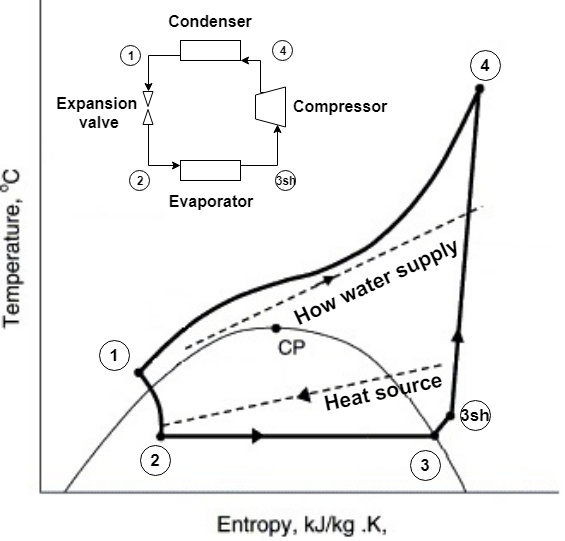
\includegraphics[width=0.5\textwidth]{HP_cylce_CO2.png}
	\caption{Temperature–entropy diagram of a trans-critical CO2 heat pump system for a domestic hot water production. Source:~\cite{kimPerformanceTranscriticalCO22005}}
	\label{fig:hp_CO2}
\end{figure}

In traditional heat pumps, the heat delivery occurs through condensation of the refrigerant, which happens at a fixed temperature. This originates high exergy losses, especially in processes were a high temperature lift is needed in the gas cooler. Some refrigerants have the particular property of having a very low critical point. Among others, a very interesting one is CO2 - technically know as R744 -, which has a critical point at 74 bars and 31 \si{\celsius}\cite{cavalliniPropertiesCO2Refrigerant2004}. As explained in Section~\ref{ss:5gden}, CO2 is also a very interesting choice for environmental and financial reasons.\\

The supercritical cycle is shown in Figure~\ref{fig:hp_CO2}, represented on the temperature-entropy diagram. The different steps of the process are explained hereafter: 
\begin{description}
\item [1 - 2]: Expansion to low pressure level
\item [2 - 3]: Evaporation by cooling down the heat source
\item [3 - 3sh]: Superheating in evaporator
\item [3sh - 4]: Compression to transcritical pressure
\item [4 - 1]: Gas cooling in transcritical area, to heat water
\end{description}
Note that, as there is no phase change, the heat exchanger is called gas cooler, instead of condenser.\\

Even though the technological development is slowly closing the gap, CO2 compressors have lower isentropic efficiency and lower volumetric efficiency than subcritical ones~\cite{sarkarSimulationTranscriticalCO22006}. This comes from the high irreversibility caused by the superheated vapor horn and the high throttling losses~\cite{yangTheoreticalExperimentalInvestigation2016}. 
However, transcritical operation also allows heat to be exchanged on a varying temperature, and the heat pump can be designed to fit the heat demand stream, optimizing exergy efficiency. This is particularly interesting in exchanges that require high temperature lifts, as in the case of domestic hot water heaters. In fact, this can be seen in Figure~\ref{fig:hp_CO2}, between point 4 and 1.  For instance, Stene et al. show that COP for a CO2 HP is lower if it is used in subcritial range - for Space Heating (SH) (35/30 \si{\celsius}) - than in supercritical range - Domestic Hot Water (DHW) (10/60 \si{\celsius}) -, despite the much higher temperature difference. They also show that the resulting COP for DHW application outperforms conventional HPs~\cite{steneINTEGRATEDCO2HEAT2007}.\\

For the transcritical CO2 heat pump, the numerical values of the compressor efficiencies computed with help of the relations obtained by Wang et al~\cite{wangExperimentalInvestigationAirsource2013}:
\begin{align}
	& \eta_{mech} = 0.64107+0.07487\cdot(\frac{P_{d}}{P_{s}})\\
	& \eta_{is} = 0.8014-0.04842\cdot(\frac{P_{d}}{P_{s}})\\
\end{align}

The procedure to evaluate the operating conditions of the heat pump is the following:
\begin{enumerate}
	\item calculate thermodynamic state in (1) with help of the temperature at the outlet of the condenser $T = T_{cond,out} = 15.5 \si{\celsius}$, optimized for this specific cycle by Henchoz et al.\cite{henchozPerformanceProfitabilityPerspectives2015}, and the pressure $P_{cond,out} = 84.9 bar$, optimized to satisfy the required inlet temperature of the condenser
	\item calculate thermodynamic state in point (3) knowing the evaporation temperature $T_{evap}$ and assuming saturated liquid
	\item calculate isentropic efficiency of compressor $\eta_{c,is}$, knowing the discharge pressure $P_{1}$ and the suction pressure $P_{3}$
	\item calculate thermodynamic state in (4is), assuming an isentropic compression with $S_{3sh}$ and $P_{1}$
	\item calculate thermodynamic state in (4), accounting for the isentropic efficiency of the compressor $\eta_{c,is}$, using $H_{4} = H_{3sh} + \frac{H_{4is} - H_{3sh}}{\eta_{c,is}}$, and $P_{cond,out}$.
	\item calculate thermodynamic state in (2), assuming isenthalpic expansion of the valve, with $H_{2} = H_{1}$ and $P_{3}$
\end{enumerate}

The equations to calculate electrical power of the heat pump and its COP, are the same as in Section~\ref{sss:hp_thermo}.

\subsubsection{Outdoor condensing unit}\label{sss:cooling_tower}
An outdoor condensing unit is an equipment used to cool down a hot stream through the ambient air. This is used in air-cooled air conditioning or refrigeration systems, to evacuate the heat into the environment. It consists of a set of fans that blow the air through a heat exchanger. These fans originate a parasitic power consumption~\cite{henchozPotentialRefrigerantBased2016} that can be calculated with help of the following equation:
\begin{equation}
\dot{E}_{fans} = \frac{0.605 \cdot \dot{Q}_{cond}}{( \Delta T_{air} + \Delta T_{min}^{ref/air})^{0.9937}}
\end{equation}
where $\dot{Q}_{cond}$ is the heat to be dissipated in the environment by the condenser. 


\subsubsection{Geo-cooling}
Geo-cooling is the use of fresh temperatures of the ground for space cooling. This happens by simply circulating a fluid between the buildings, where the heat is extracted, and the geothermal wells, where heat is released into the ground. In practice, this happens by bypassing the heat pumps and making the water of the secondary loop (geothermal loop) directly exchange with the heating water loop. Investment costs are, thus, limited to an additional heat exchanger. 

The energy needed for circulation pumps is assumed to be negligible. 


\subsubsection{PV}\label{sss:pv}
The efficiency of the PV panels $\eta_{PV}$ is given by the following equation~\cite{stadlerModelbasedOptimizationDistributed2016}:
\begin{equation}
	\eta_{PV} = \eta_{ref} - \eta_{var} (T_{panel}-T_{ref})
\end{equation}
where $\eta_{ref}$ and $\eta_{var}$ are respectively the fixed efficiency and the temperature dependent efficiency. The temperature of the panel $T_{panel}$ is calculated by means of:
\begin{equation}
	T_{panel} = \frac{U_{glass}\cdot T_{amb} + GI \cdot f_{glass}-\eta_{ref} - \eta_{var} \cdot T_{ref}}{U_{glass}-\eta_{var} \cdot GI}
\end{equation}
where $U_{glass}$ is the thermal transmittance of the front glass, $f_{glass}$ is the light transmittance of the front glass and GI is the global irradiation.
Thus, the produced energy is given by:
\begin{equation}
	E = GI \cdot A_{PV} \cdot  \eta_{PV}
\end{equation}
The area of installed PV $A_{PV}$ is expressed in function of the total roof area of the buildings $A_{roof}$:
\begin{equation}
	A_{PV} = A_{roof} \cdot f_{area}
\end{equation}
where the area factor $f_{area}$ is the ratio between the available roof area and the area of PV that can be installed, accounting for the optimal distance between the panels, obstacles and margins. This value can vary depending on the type of roof, type of PV panels and orientation of the building.

\subsubsection{Network}\label{sss:net}
The length is calculated, according to a simplified method~\cite{girardinEnerGisGeographicalInformation2010}:
\begin{equation}
L = 2(n_{b}-1)K\sqrt{\frac{S}{n_{b}}}
\end{equation}
with $S$ being the land area, $n_{b}$ the number of buildings. The constant $K$ is chosen at 0.5.
And diameter of the pipes:
\begin{equation}
d = \sqrt{\frac{4\cdot \dot{m}}{\pi v_{s} \rho}}
\end{equation}
assuming a sizing velocity $v_{s}$ of 3 m/s, calculated to be the maximum velocity of liquid flow in pipelines of 300-500 mm diameter that avoids rapid aging caused by abrasion, cavitation and fatigue~\cite{henchozPerformanceProfitabilityPerspectives2015}.
The investment costs are calculated accordingly:
\begin{equation}
C = \sum_{k=1}^{n_{b}} \frac{L}{n_{b}} (c_{1} d \sqrt{n_{b}+1-k} + c_{2})
\end{equation}
where $c_{1} =5670 $ and $c_{2} = 613 $.\\

Operating temperature is assumed to be 13 \si{\celsius} for the liquid pipe and 15 \si{\celsius} for the vapor pipe~\cite{suciuEnergyautonomousCitiesUsing2016}.\\

The pressure losses, and thus the energy needed for the maintaining of the pressure, are assumed to be negligible.

\subsection{MILP optimization and Osmose}\label{ss:osmose}

Mixed integer linear programming (MILP) is a mathematical optimization, in which some variables are restricted to be integers, while other are discrete. A MILP model can be written with AMPL (A Mathematical Programming Language), which is a modeling language specifically designed to describe and solve optimization problems. Once defined the model, this is passed to a solver, as for example Gurobi or GLPK, which solves the given problem.\\

Osmose is a platform developed at IPESE for the study and the design of complex integrated energy systems. Its aim is to allow the user to model and compute an optimization problem using the same platform, which would normally require to access and transfer data between several programs. The coding language is \textit{lua}.

Osmose allows to define a model for the different energy conversion technologies that want to be analyzed. It will then prepare the necessary files for the optimization of the energy system that will be handed over to AMPL. After the solving is complete, the results sent back to Osmose, allowing to post-process the data to run sensitivity analysis, multi-objective optimizations or simply calculate performance indicators.\\

In first place, energy technologies have to be defined, with its set of equations that determine the supply and the demand of the unit. Moreover it is necessary to furnish the following cost parameters:
\begin{itemize}
	\item $c^{inv1}$: fixed part of the IC, given in $[CHF/year]$. This can be found in Figure~\ref{fig:lin} in Section~\ref{ss:ic};
	\item $c^{inv2}$: variable part of the IC, given in $[CHF/year]$. This can be found in Figure~\ref{fig:lin} in Section~\ref{ss:ic};
	\item $c^{op1}$: fixed part of the OC, which corresponds to maintenance and service costs. 
	\item $c^{op2}$: variable part of the OC. This is the operating cost resulting from the system optimization, also in $[CHF/h]$.
\end{itemize}

The sizing of the energy conversion technologies is constrained with the following equations~\cite{suciuEnergyIntegrationCO22018}:
\begin{align}
& f_{u,t} \leq f_{u} \qquad \forall u \in U, \ \forall t \in T  \\
& f_{u}^{min} \cdot y_{u} \leq f_{u} \leq f_{u}^{max} \cdot y_{u} \qquad \forall u \in U\\
\end{align}
where $U$ is the set of units, and $T$ is the set of operating times.

For \textit{process units} - i.e. the subset of units U with a defined sizing, as for example the units in the industrial production line of a product - $y_{u} = f_{u}^{min} = f_{u}^{max} = 1$. In a residential district only the houses, which are defining the energy demand, are considered as \textit{process units}.\\

The total cost of the system is given by:
\begin{align}
& \sum_{u}^{U} \left[ \sum_{t = 1}^{T} \left( c_{u}^{inv1} \cdot y_{u,t} + c_{u}^{inv2} \cdot f_{u,t} + c_{u}^{op1} \cdot y_{u,t} + c_{u}^{op2} \cdot f_{u,t} \right) \cdot t_{t}^{op} \right] \\
\end{align}

A set of equations, called heat cascade, makes sure that heat is always transferred from a higher temperature to a lower one, also considering the respective minimum approach temperature for each stream.
\begin{align}
& \sum_{u}^{U} f_{u,t}  \cdot \dot{Q}_{u,t,k} + \dot{R}_{t,k+1} - \dot{R}_{t,k} = 0 \qquad \forall k \in K, \ \forall t \in T \\
& \dot{R}_{t,k} \geq 0 \qquad \forall k \in K, \ \forall t \in T  \\
& \dot{R}_{t,1} = \dot{R}_{t,k+1} = 0 \qquad \forall t \in T  \\
\end{align}
where $K$ is the set of temperature intervals.

The demand $\dot{m}_{r,u,t}^{+}$ and the supply $\dot{m}_{r,u,t}^{-}$ of resource $r \in R$ of each unit $u \in U$ is computed:
\begin{align}
& \dot{M}_{r,u,t}^{-} = \dot{m}_{r,u,t}^{-} \cdot f_{u,t} \qquad \forall r \in R, \ \forall u \in U, \ \forall t \in T \\
& \dot{M}_{r,u,t}^{+} = \dot{m}_{r,u,t}^{+} \cdot f_{u,t} \qquad \forall r \in R, \ \forall u \in U, \ \forall t \in T  \\
\end{align}
where $R$ is the set of resources. 
The balance of each resource has to be respected:
\begin{equation}
\sum_{u}^{U} \dot{M}_{r,u,t}^{-} = \dot{M}_{r,u,t}^{+} \qquad \forall r \in R, \ \forall t \in T
\end{equation}
Electricity is also balanced:
\begin{equation}
\dot{El}_{houses}^{+} + \dot{El}_{heating}^{+} + \dot{El}_{cooling}^{+} + \dot{El}_{grid}^{+} = \dot{El}_{PV}^{-} + \dot{El}_{grid}^{-}
\end{equation}

The objective function defines which parameters have to be maximized or minimized during the optimization process. It is common to choose to minimize either the operating, the investment costs or a combination of them. However, other parameters, as for example the amount of carbon emissions, can be considered.



\newpage
\section{Application}

\subsection{Case-study Eglantine}\label{ss:Eglantine}
In the framework of the collaboration between Romande Energie and IPESE, a case study shall bring a concrete numerical case study into the discussion. For this, Romande Energie has chosen a real life example of a district in the city of Morges. This district is in the planning phase, and Romande Energie had worked on it, in order to participate in the call for tender. This case study shall be fertile ground to discuss the CO2 DEN technology and its role in the future energy systems in Switzerland and, more particularly, in the future plans of Romande Energie.

\subsubsection{Context}

\begin{figure}[htp]
\centering
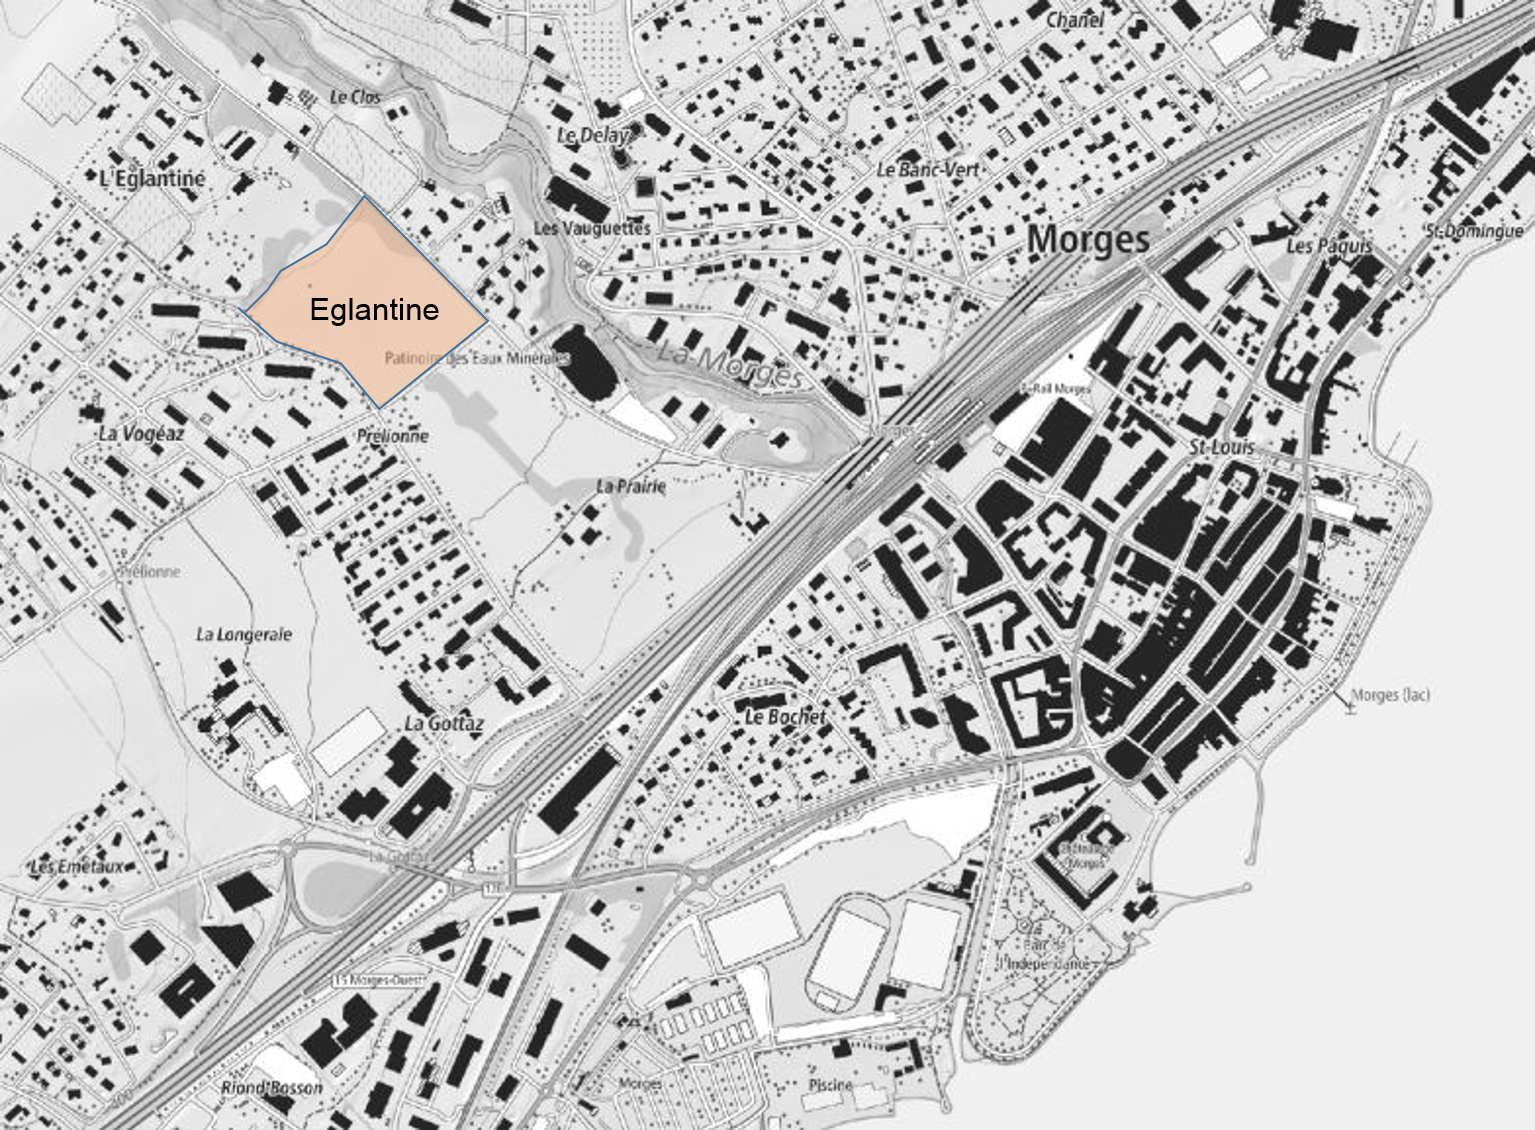
\includegraphics[width=1\textwidth]{morges.png}
\caption{Localization of the terrain, at the town scale. Source:~\cite{GuichetCartographiqueEtat}}
\label{fig:morges}
\end{figure}

The “Eglantine” is a terrain in the western part of the city of Morges, as shown in Figure~\ref{fig:morges}. It is located in the proximity of key urban facilities, as well as the countryside. This terrain, which was partly used for agriculture, and partly covered by rich vegetation, belongs to the municipality, who is planning to use it for the urban expansion. The municipality had the vision of building a new district, which would be planned to be exemplary in the sustainable development. After many years of revising and fine-tuning the land-use plan and its vision for the future, in the beginning of 2016, the commune launched a call for tender for the planning of the different aspects of the district. The call for tender regarding the energy system was opened by Losinger Marazzi the 1st December 2017, with a due date the 31 January 2018. The contract with the winner, unknown to the author, has been signed in the end of March 2018. \\

The call for tender requires the development of a complete energy system, including thermal and electrical energy. Estimated data about the buildings is provided and can be cound in Appendix~\ref{as:eglantine}. Those are based on the following assumptions:
\begin{itemize}
    \item All buildings are certificated Minergie 2017
    \item Space heating and hot water energy demand follow the SIA 380/1 and SIA 2031 norms
    \item Air ventilation is defined according to Minergie 2017 principles.
    \item Installed power values are calculated according to SIA 2024 norm
\end{itemize}

\subsubsection{Available data}
The district, which will host around 1'500 people, is composed of fourteen buildings, as shown in Appendix~\ref{as:eglantine}, which account for a total energy reference area (ERA) of around $47'000 m^{2}$. The details are shown in Table~\ref{tab:ppa_summary_tot}. According to the Minergie standard, the district will require about $1.40 MWh/yr$ for SH and $0.95 MWh/yr$ for DHW.\\

\begin{table}[h!]
\centering
\caption{Estimated energy demand in call for tender}\vspace{2mm}
\label{tab:ppa_summary_tot} 
\begin{tabular}{lrrrrr}
\toprule
\textbf{Buildings} & \begin{tabular}[c]{@{}l@{}}\textbf{Energy Ref.} \\ \textbf{Area (ERA)}\end{tabular} & \textbf{Inhabitants} & \begin{tabular}[c]{@{}l@{}}\textbf{Space Heating} \\ \textbf{(SH)}\end{tabular}                                             & \begin{tabular}[c]{@{}l@{}}\textbf{Hot Water} \\ \textbf{(DHW)}\end{tabular} & \textbf{TOTAL}     \\
         &                                                                        &             & \begin{tabular}[c]{@{}l@{}}MIINERGIE\\ simple flux\end{tabular} & SIA 380/1       &           \\ 
         & [m2]                                                                   &             & [kWh/yr]                                                        & [kWh/yr]        & [kWh/yr]  \\ \midrule
   
\textbf{13}      & \textbf{46'350}                              & \textbf{1'498}       & \textbf{1'401'559}      & \textbf{948'958}         & \textbf{2'350'521} \\
\bottomrule
\end{tabular}
\end{table}

The call for tender includes also information about the end use of the buildings, which is shown in Table~\ref{tab:ppa_buildinguse_tot}. It can be seen that the buildings include, beside the residential use, also a small share of retail and restaurant services use, which are associated with different energy needs. Moreover, there is even a small indoor swimming pool, located in building one. 

\begin{table}[h!]
\centering
\caption{Total estimated use of buildings in call for tender}\vspace{2mm}
\label{tab:ppa_buildinguse_tot}
\begin{tabular}{lrrrr}
\toprule
\textbf{Category} & \textbf{Housing} & \textbf{Retail} & \textbf{Restaurant services} & \textbf{Indoor swimming pool} \\
                  & \textbf{[\%]}               & \textbf{[\%]}      & \textbf{[\%]}          & \textbf{[\%]}              \\
                  \midrule
\textbf{Tot}	  & 97.08 \%					& 1.63 \%			& 0.78 \%					& 0.51 \%					\\
\bottomrule
\end{tabular}
\end{table}

The energy profile of the buildings is calculated according to Minergie standard, as well as the SIA norms. Given the annual energy demand for space heating and hot water, as shown in Table~\ref{tab:ppa_summary_tot}, the monthly profile is shown in Figure~\ref{fig:ppa_energydemand}.

\begin{figure}[htp]
\centering
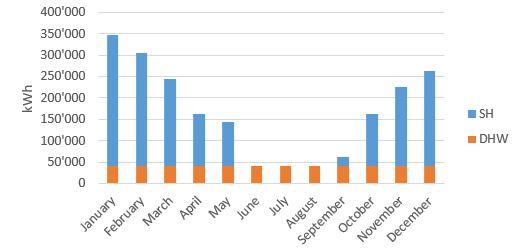
\includegraphics[width=0.8\textwidth]{ppa_energydemand.JPG}
\caption{Annual energy distribution for space heating and hot water}
\label{fig:ppa_energydemand}
\end{figure}

Some pre-studies have been commissioned by the land-owner, in order to give, on an indicative basis, the sizing of the energy system. These studies have been realized by external engineering firms and the results are contained in the call for tender. The studied parameters include the sizing for heat pumps, geothermal wells, as well as PV, and are shown in Table~\ref{tab:ppa_prestudy_tot}. They estimate a PV potential on the building roofs of $570 kWp$, and the need for an installed heating power of $1'258 kW$, using 77 geothermal wells of an average length of $271 m$

\begin{table}[h!]
\centering
\caption{Estimated sizing of energy system in call for tender}\vspace{2mm}
\label{tab:ppa_prestudy_tot} 
\begin{tabular}{lrrrr}
\toprule
\textbf{} & \textbf{HP}    & \textbf{PV}    & \multicolumn{2}{l}{\textbf{Geothermal}} \\
         &       &       & \textbf{Nb. wells}        & \textbf{Average Depth}        \\
         & \textbf{[kW]} & \textbf{[kWp] } &                 & \textbf{[m] }         \\ \midrule
\textbf{TOT}      & \textbf{1'258}   & \textbf{570} & \textbf{77}              &    \textbf{267}         \\
\bottomrule
\end{tabular}
\end{table}

Detailed data from the call for tender can be found in the Appendix~\ref{as:eglantine}.

\subsubsection{Energy demand - Typical days}
The profile of the energy demand is calculated as explained in Section~\ref{ss:typicalDays}. The used threshold temperature for heating is $T_{th}^{heat} = 14\si{\celsius}$ and for cooling $T_{th}^{cool} = 18 \si{\celsius}$. The resulting energy demand, already multiplied by the number of occurrencies for each time step, is shown in Figure~\ref{fig:energyDemand}.

\begin{figure}[h!]
	\centering
	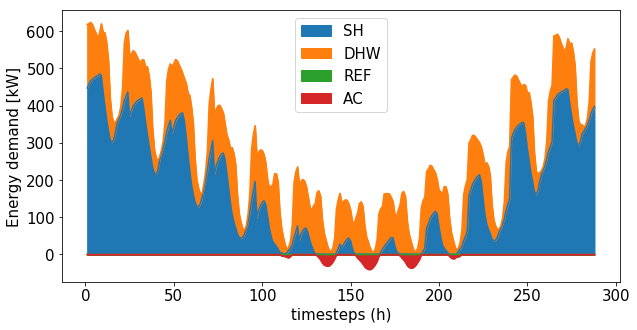
\includegraphics[width=0.8\textwidth]{energy_demand.png}
	\caption{Total heating (+) and cooling (-) demand of the Eglantine district, for each time step}
	\label{fig:energyDemand}
\end{figure}


\subsection{Heat sources}
The heat pumps in a system can source heat from various sources. Its choice depends on the source temperatures and its investment costs. This chapter illustrates the different heat sources that have been considered in this work.

\subsubsection{Stream}
A small stream flows along the eastern boundary of the area, on which the Eglantine district is being built. However, the flow rate would not be sufficient to cover the heating/cooling demand, especially during the dry winter season~\cite{veillehydro-meteorologiqueducantondevaudMorgesRiviere}. For example, the lowest value has been reached in August 2004 with $0.017 m^3/s$, and even in December 2005 the lowest daily flow was of $0.057 m^3/s$. \\
For this reason, the stream has been excluded from further analysis and has not been considered as a viable solution.

\subsubsection{Lake}
Lake water is commonly sourced at a depth of around 70 m, where a constant temperature of 7.5\si{\celsius} is found throughout the year. This water is led to the central pump through a water pipe. The massflow of the water is calculated in order to satisfy a drop/rise in the water stream of $\Delta T_{water}  = 4 \si{\celsius}$.

The cost function is calculated as for the CO2 pipes (see Section~\ref{sss:net}), considering the needed diameter to satisfy the heating/cooling demand, which depend on the different heat capacity and massflow of the water. The length of the pipes, which is measured on a GIS software, is of 1'500 m.


\subsubsection{Geothermal wells}
The average temperature of a geothermal well is calculated according to Section~\ref{ss:gtw}. The temperature gradient in the lemanic region is found in experimental data from Geneva canton~\cite{gadzEvaluationPotentielGeothermique2011}: $\nabla T_{g} = 0.03 [K/m]$ (see Figure~\ref{fig:gtwgrad} in Appendix~\ref{as:gt}).
This value also corresponds to the average gradient found in the Swiss plateau~\cite{siaSIA384Sondes2010}.

The average surface temperature depends mainly on the latitude and on the altitude. Standard values for different regions of Switzerland can be found in the SIA norm 384~\cite{siaSIA384Sondes2010}. Experimental measurements~\cite{gadzEvaluationPotentielGeothermique2011} show that the surface temperature in the lemanic region is $	T_{g,s} = 11 \si{\celsius}$ (see Figure~\ref{fig:gtwts} in Appendix~\ref{as:gt}).

Knowing the average depth of the geothermal wells, which is found to be $L_{gtw} = 267$ (see Section~\ref{ss:Eglantine}), the mean temperature in the geothermal well corresponds to $T_{g, mean} = 15 \si{\celsius}$.

It is assumed that the geothermal wells are well sized, in order to respect the natural recharge rate, which is strongly dependent on the type of soil. The sizing of the boreholes is very important to ensure a sustainable use of the ground heat throughout the years. \\

\begin{figure}[htp]
	\centering
	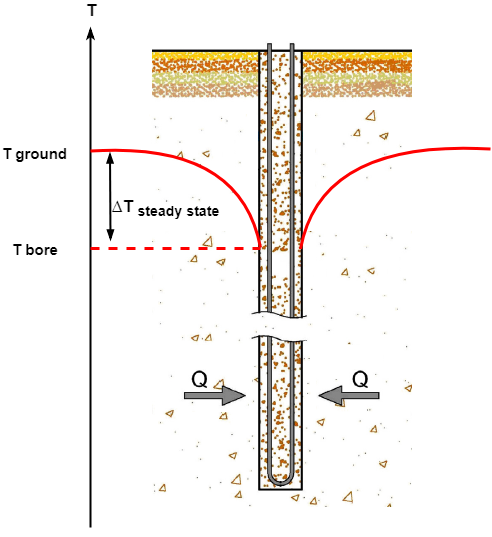
\includegraphics[width=0.5\textwidth]{GTW_T_profile.png}
	\caption{Steady state temperature difference in borehole, due to heat extraction}
	\label{fig:GTW_T}
\end{figure}

At any time heat is extracted from the ground, there is a temperature gradient that will form around the borehole, as shown in Figure~\ref{fig:GTW_T}. This temperature gradient depends on the heat extraction rate and the conductivity of the soil. Given the energy demand of the Eglantine district, it has been chosen to assume a negative temperature difference ($\Delta T_{steady state}$) of 3 \si{\celsius}~\cite{guoTechnoeconomicComparisonDirect2012,hanSensitivityAnalysisVertical2016}, due to the reduced cooling demand for this application. Thus the mean useful temperature of the borehole over its depth is given by:
\begin{equation}
	T_{b, mean} = T_{g, mean} -\Delta T_{Steady State} = 12 \si{\celsius}
\end{equation}
It has to be noted that this temperature gradient would be positive if the cooling demand is larger than the heating demand, thus resulting in an increase of the ground temperature.\\

The price for boreholes in Switzerland is found to be around $c_{wells} = 80$ [CHF/m]~\cite{bawos.chMitErdsondenbohrungenKosten2018}. 
In order to provide the model with an energy dependent cost function, this value is transformed with help of the data from Table~\ref{tab:ppa_prestudy} in Appendix~\ref{as:eglantine}:
\begin{align}
&  L_{wells}^{tot} = n_{wells} * L_{well}^{average} \\
& 	\text{Cost function [CHF/kW]} = c_{wells} \frac{L_{wells}^{tot}}{P_{hp}^{tot}}
\end{align}
where $L_{wells}^{tot}$ is the length and $n_{wells}$ the number of boreholes, and $P_{hp}^{tot}$ is the total power of heat pumps installed. 

The investment cost is calculated for summer use - the heat dissipated - as well as for the winter use - heat extracted, in function of the peak load of heating/cooling required. However, in reality the system is accounting twice for the same borehole, since the one for winter use will be the same during winter use. Thus, the total cost for the geothermal wells is chosen as the larger value between the two:
\begin{equation}
IC_{GTW} = 	\max \left( IC_{GTW}^{summer}, IC_{GTW}^{winter} \right) 
\end{equation}

The minimum approach temperature, necessary to exchange heat with the soil, can be determined with help of the procedure described in Section~\ref{ss:dtmin}. 
The cost of the heat exchange area of the borehole is calculated assuming a standard pipe diameter of $32 mm$\cite{siaSIA384Sondes2010, kruseStatusDevelopmentResearch2010}.
The overall heat transfer coefficients of the well - including the fluid, the bore wall and the soil - are assumed to be~\cite{kruseStatusDevelopmentResearch2010}:
\begin{align}
	& U^{g/water} = 9.3 kW/m^2K
	& U^{g/CO2} = 17.1 kW/m^2K
\end{align}

The resulting minimum approach temperatures are:
\begin{align}
	&\Delta T_{min}^{g/water} = 14 \si{\celsius}
	&\Delta T_{min}^{g/CO2} = 6.8 \si{\celsius}
\end{align}
These values are similar to experimental or standard values found in literature~\cite{siaSIA384Sondes2010, lamarcheReviewMethodsEvaluate2010}.\\

The water rise/drop in the water ground loop is assumed to be $dT_{water} = 4 \si{\celsius}$~\cite{siaSIA384Sondes2010}\\


\subsection{External heat sources}
The main advantage of a 5th generation district heating network is the ability to recover heat, and exchange it among the diversity of users. 
Two potential heat sources have been identified in the surroundings of the Eglantine district: the ice rink and a shopping mall. For the scope of this work, only the ice rink has been considered and studied.

\subsubsection{Ice rink}

\begin{figure}[htp]
	\centering
	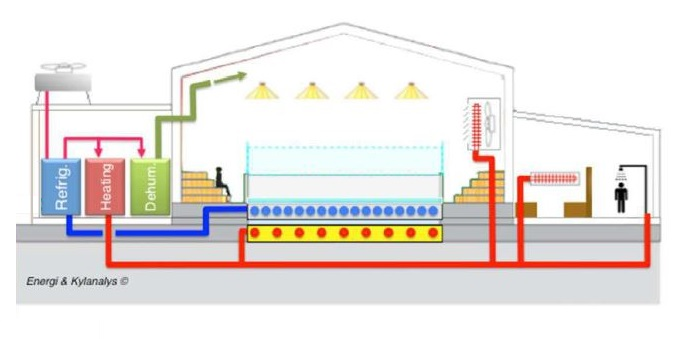
\includegraphics[width=0.8\textwidth]{IR_schema.JPG}
	\caption{Energy system of a typical ice rink~\cite{gronqvistComparativeLifecycleCost2016}}
	\label{fig:IR_schema}
\end{figure}

An ice rink is a place where people can ice skate and play winter sports. The ice surface is normally inside an arena, which ensures comfortable temperatures for the people on the ice, as well as for the public, throughout the season. This also allows to extend the season, avoiding ice melt, when temperatures are warmer outside.\\

A study, conducted on more than one hundred ice rinks in Sweden, shows that the refrigeration system used to cool the ice surface has the largest share in total energy consumption, 43\% (in average) as indicated in Figure~\ref{fig:IR_energyDemand}~\cite{kolasniewskiEvaluationModellingIce2017}.
However, the ice rink often also includes changing rooms with showers, and a cafeteria or a restaurant, which also present heating demand. According to Figure~\ref{fig:IR_energyDemand}, the average share of heating in the total energy demand is 26\%.
Last but not least, the ice surface has to be constantly illuminated, which requires a powerful lightning system. The global system is shown in Figure~\ref{fig:IR_schema}.\\

However, for practicality reasons, it is assumed that only the refrigeration system is connected to the CO2 network, while the heating and electricity demand is supplied by the existing system, and are thus not considered in this model.

\begin{figure}[htp]
	\centering
	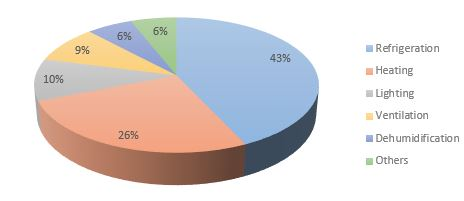
\includegraphics[width=0.7\textwidth]{IR_energyDemand.JPG}
	\caption{Energy demand of a typical ice rink~\cite{kolasniewskiEvaluationModellingIce2017}}
	\label{fig:IR_energyDemand}
\end{figure}

Ice rinks are conventionally cooled with indirect systems, as shown in the right part of Figure~\ref{fig:IR_refSystem}, based on a ammonia (NH3) vapor compression chiller, exchanging with a secondary brine loop that extracts the heat from the ice surface. The waste heat is normally, or at least in older systems, exchanged with the environment, with help of outdoor condensing units. Connecting it to a 5th generation district heating network, would allow recovering this heat and use it to cover the heat demand of other users. The connection to the CO2 network is shown in the left part of Figure~\ref{fig:IR_refSystem}. This presents a high energy and exergy efficiency gain, since the refrigeration system can be driven on a lower and constant condensation temperature. However, assuming to recover heat from an existing cooling system, this gain is not considered in this work.\\

\begin{figure}[htp]
	\centering
	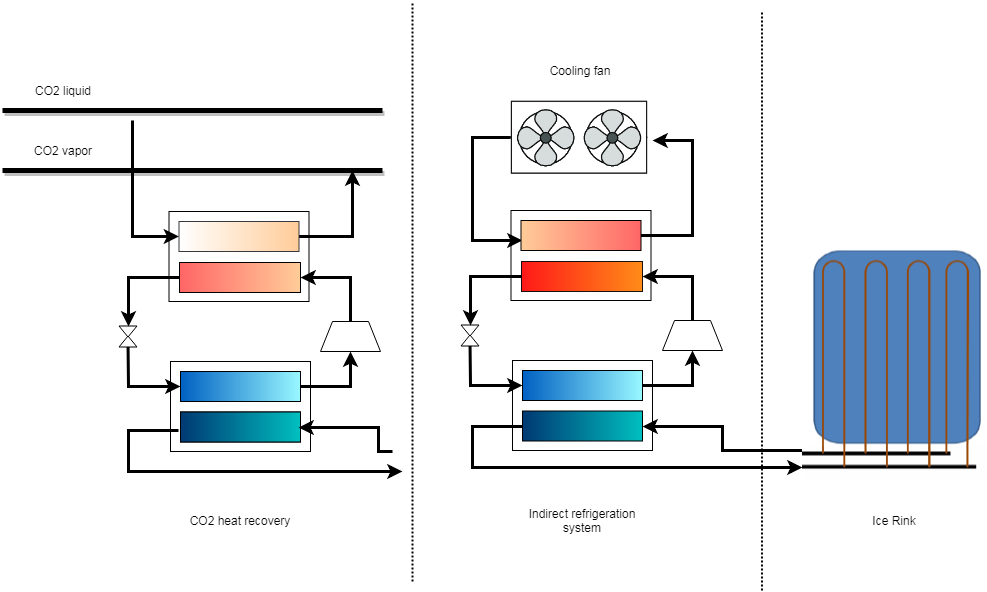
\includegraphics[width=1\textwidth]{IceRink_refrigeration.png}
	\caption{Refrigeration systems for ice rinks}
	\label{fig:IR_refSystem}
\end{figure}

The calculation of the cooling demand of the ice rink is based on the following assumptions:
\begin{itemize}
	\item Constant load profile throughout the ice season
	\item Ice season: 1st of August - 1st of April
	\item $COP_{ref} = 4$~\cite{kolasniewskiEvaluationModellingIce2017}
	\item Ice surface = $1800m^2 $~\cite{kolasniewskiEvaluationModellingIce2017}
	\item Specific cooling demand = $1kWh/m^2/day$~\cite{kolasniewskiEvaluationModellingIce2017}
	\item $dT_{min}(refrigerant-ice) = 1 \si{\celsius}$
	\item $dT_{min}(refrigerant-refrigerant) = 3 \si{\celsius}$
\end{itemize}

The daily cooling demand profile of the ice rink, is based on the required ice temperature, which varies throughout the day~\cite{kolasniewskiEvaluationModellingIce2017}, as shown in Figure~\ref{fig:IR_load}. Thus the computed ice cooling load profile is shown in Figure~\ref{fig:IR_profile}.

The total resulting waste heat rejected by the ice rink throughout the year corresponds to about $ 450 MWh/year$.

\begin{figure}[!htb]
	\centering
	\begin{minipage}{.45\textwidth}
		\centering		
		\begin{tabular}{lll}
			\toprule
			\textbf{Period} & \textbf{Rink function} & \textbf{\begin{tabular}[c]{@{}l@{}}$T_{ice}$\\ {[}\si{\celsius}{]}\end{tabular}} \\
			\midrule 
			0.00-6:00   & Night setback   & -1     \\
			6:00-8:00   & Ice maintenance & -1     \\
			8:00-16:00  & Low load        & -3     \\
			16:00-18:00 & Figure skating  & -4     \\
			18:00-24:00 & Hockey          & -6    \\
			\bottomrule
		\end{tabular}
		\caption{Ice rink refrigeration profile}\vspace{2mm}
		\label{fig:IR_load}
	\end{minipage}%
	\hspace{1cm}
	\begin{minipage}{0.45\textwidth}
		 \centering
		 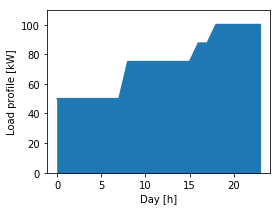
\includegraphics[width=\linewidth]{Images/IR_profile}
		 \caption{Ice cooling load profle of the ice rink, for a typical day}
		 \label{fig:IR_profile}
	\end{minipage}
\end{figure}

%\begin{table}[h]
\centering
\label{tab:IR_profile}
\caption{Ice rink refrigeration profile}\vspace{2mm} 
\begin{tabular}{lll}
\toprule
\textbf{Period} & \textbf{Rink function} & \textbf{\begin{tabular}[c]{@{}l@{}}$T_{ice}$\\ {[}\si{\celsius}{]}\end{tabular}} \\
\midrule 
0.00-6:00   & Night setback   & -1     \\
6:00-8:00   & Ice maintenance & -1     \\
8:00-16:00  & Low load        & -3     \\
16:00-18:00 & Figure skating  & -4     \\
18:00-24:00 & Hockey          & -6    \\
\bottomrule
\end{tabular}
\end{table}

%\begin{figure}[tph]
%	\centering
%	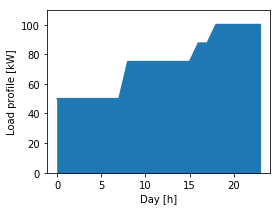
\includegraphics[width=0.45\linewidth]{Images/IR_profile}
%	\caption{Ice cooling load profle of the ice rink, for a typical day}
%	\label{fig:IR_profile}
%\end{figure}

\subsection{PV}\label{ss:pv}
The area factor $f_{area}$ (see Section~\ref{sss:pv}) for flat roofs is assumed to be $\frac{1}{4}$.

The optimizer chooses the amount of PV that has to be installed ($f_{u}^{PV}$), according to the chosen objective function and parameters. This decision variable is sized to the total available roof area (see Section~\ref{sss:pv}). In some cases $f_{u}^{PV}$ has been limited to 1, in order to let the optimizer use the total roof area, while in some other cases $f_{u}^{PV}$ has been limited to 2, assuming that additional area (facades, parking lots, free area, etc.) would be available for the installation of PV panels. 
Table~\ref{tab:pv} shows the resulting PV area $A_{PV}$ for those numerical examples.
%\todo{check roof area in model}

\begin{table}[htp]
	\centering
	\caption{Numerical examples for PV area $A_{PV}$, in function of the available roof area $A_{roof}$ and the decision variable of the optimizer $f_{u}^{PV}$ (see Section~\ref{ss:osmose}).}
	\label{tab:pv}
	\begin{tabular}{lrr} \toprule
		$f_{u}^{PV}$			& 1	& 2\\  \midrule
		$f_{area}$	 & 0.25	& 0.25 \\
		$A_{roof}$          & 8680 $m^2$   & 8680 $m^2$ \\
		\textbf{$A_{PV}$}	 & \textbf{	2170 $m^2$}	& \textbf{4340 $m^2$}\\ \bottomrule
	\end{tabular}
\end{table}

\subsection{Energy conversion technologies}
In order to evaluate the potential of alternative energy systems, three energy systems have been defined:
\begin{enumerate}
	\item GS-HP: a set of decentralized geothermal heat pumps for heating, geo-cooling for space cooling and air-cooled compression chillers for refrigeration
	\item GS-CO2DEN: CO2 based district energy network, with a central plant exchanging heat with the environment through a geothermal field
	\item LS-CO2DEN: CO2 based district energy network, with a central plant exchanging heat with the environment through lake water
\end{enumerate}

\subsubsection{GS-HP}
This energy conversion technology corresponds to a state of the art energy system for buildings and district, which is widespread in new buildings. Its schema is shown in Figure~\ref{fig:energyschemaref}

\begin{figure}[tph]
	\centering
	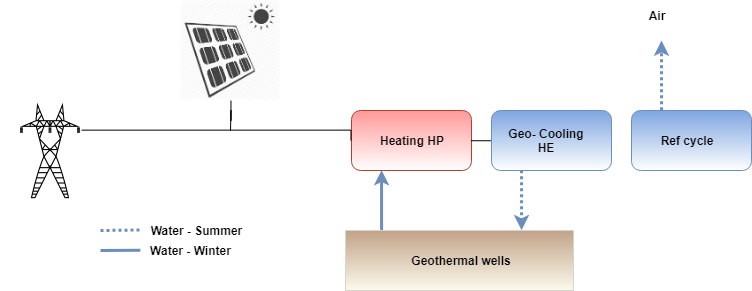
\includegraphics[width=1\linewidth]{Images/energy_schema_ref}
	\caption{Schematic view of the GS-HP energy conversion system}
	\label{fig:energyschemaref}
\end{figure}

The resource flows of the different units in the system are shown in Table~\ref{tab:layers_ref}.
\begin{table}[h!]
	\centering
	\caption{Resource flows for the reference energy system ((-): flow in / (+): flow out))}\vspace{2mm}
	\label{tab:layers_ref} 
	\begin{tabular}{lccc}
		\toprule
		& \multicolumn{3}{c}{Resource flows}             \\
		Units          & Electricity & $Source_{hot}$ & $Source_{cold}$ \\ \midrule
		$HP_{sh}$      & -           & -              & +               \\
		$HP_{dhw}$     & -           & -              & +               \\
		$HP_{ref}$     & -           & +              & -               \\
		$HE_{ac}$      &             & +              & -               \\
		Elec. Heater   & -           &                &                 \\
		PV             & +           &                &                 \\
		$GTW_{winter}$ &             & +              & -               \\
		$GTW_{summer}$ &             & -              & +              \\ \bottomrule
	\end{tabular}
\end{table}




The heating demand is supplied by a set of decentralized geothermal heat pumps, one for domestic hot water and one for space heating in every building. These heat pumps source the ambient heat from a secondary loop that exchanges heat with the ground through a system of geothermal wells, the SL-GSHP, which is described in Section~\ref{ss:dx}. 

Given the relevance of the heat pumps in the studied energy system, it has been chosen to use its thermodynamic model, which achieves more reliable and precise results.\\

The temperatures at the evaporator and condenser are given by the following equations:
\begin{equation}
    T_{evap} = T_{ground} - \Delta T_{min}^{ground/water} - \Delta T_{water} - \Delta T_{min}^{ref/water}
\end{equation}
\begin{equation}
    T_{cond} = T_{demand} + \Delta T_{min}^{ref/water}
\end{equation}
where $\Delta T_{min}$ are the corresponding minimum approach temperatures, and $\Delta T_{water}$ is the temperature rise in the secondary water loop exchanging with the ground.

For the space heating heat pump, the refrigerant used is R123yf, as described in Section~\ref{sss:hp_thermo}.

For the domestic hot water, it is chosen to use transcritical CO2 heat pumps. As described in Section~\ref{sss:hp_CO2}, this technology can achieve very good performances supplying heat that requires a high lift. This is the case in domestic hot water, where the water has to be heated from a temperature of 10 \si{\celsius} to a temperature of 55 \si{\celsius}.\\

Given the availability of geothermal wells, it has been chosen to implement geo-cooling for space cooling. The system is providing cooling at the ground temperature, corrected with the minimum approach temperature $\Delta Tmin_{ground/water}$ and the temperature rise in the water loop $\Delta T_{water}$.
\begin{equation}
T_{geo-cooling} = T_{ground} + \Delta T_{min}^{ground/water} + \Delta T_{water}
\end{equation}

The refrigeration is achieved with a set of decentralized air cooled vapor compression chillers, which present the same working principle as heat pumps. The heat is evacuated into the environment with help of outdoor condensing units, as described in Section~\ref{sss:cooling_tower}.
The total energy consumption of the chillers is thus a sum of the energy demand of the compressor and the cooling fans:
\begin{equation}
\dot{E} = \dot{E}_{ref} + \dot{E}_{fans}
\end{equation}
and the operating temperatures are defined in the following way:
\begin{equation}
    T_{cond} = T_{amb} + \Delta T_{air} + \Delta T_{min}^{ref/air}
\end{equation}
where $T_{amb}$ is the ambient temperature, $\Delta T_{air}$ is the temperature difference of the cooling air between the input and the output of the condenser, while $\Delta T_{min}^{ref/air}$ is the minimum approach temperature difference needed for heat transfer between a refrigerant and air.\\

\subsubsection{CO2DEN}\label{sss:CO2DEN}
The schema of the CO2 network energy system is shown in Figure~\ref{fig:energyschema}, while the main resource flows are shown in Table~\ref{tab:layers_CO2}.

\begin{figure}[tph]
	\centering
	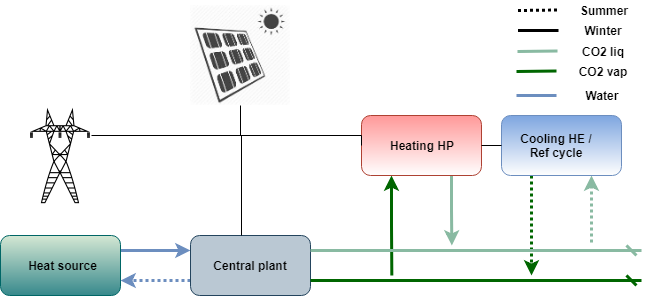
\includegraphics[width=1\linewidth]{Images/energy_schema}
	\caption{Schematic view of the CO2DEN energy conversion system}
	\label{fig:energyschema}
\end{figure}

\begin{table}[h!]
	\centering
	\caption{Resource flows for the CO2 DEN ((-): flow in / (+): flow out))}\vspace{2mm}
	\label{tab:layers_CO2} 
	\begin{tabular}{llllll}
		\multicolumn{1}{c}{-} & \multicolumn{5}{c}{Resource flows}                                          \\
		Units                 & Electricity & $CO2_{liq}$ & $CO2_{vap}$ & $Source_{hot}$ & $Source_{cold}$ \\
		$HP_{cp}^{winter}$    & -           & -           & +           & -              & +               \\
		$HP_{cp}^{summer}$    &             & +           & -           & +              & -               \\
		$HP_{sh}$             & -           & +           & -           &                &                 \\
		$HP_{dhw}$            & -           & +           & -           &                &                 \\
		$HP_{ref}$            & -           & -           & +           &                &                 \\
		$HE_{ac}$             &             & -           & +           &                &                 \\
		Elec. Heater          & -           &             &             &                &                 \\
		PV                    & +           &             &             &                &                 \\
		$GTW_{winter}$        &             &             &             & +              & -               \\
		$GTW_{summer}$        &             &             &             & -              & +              
	\end{tabular}
\end{table}


For space heating and domestic hot water, the same model as for the heat pumps in GS-HP are used. Since in this case the HP sources heat from the CO2 network instead of the geothermal wells, the mayor difference lies in the evaporation temperature, which corresponds to temperature in the CO2 vapor pipe ($T_{CO2,g}$):
\begin{equation}
    T_{evap} = T_{CO2,g} - \Delta T_{min}^{ref/ref}
\end{equation}

As for GS-HP, refrigeration is achieved through decentralized vapor compression chillers. However, in this case they are not air cooled, but they exchange directly with the CO2 network. Thus, the temperature in the condenser is given by:
\begin{equation}
    T_{cond} = T_{CO2,l} + \Delta T_{min}^{ref/CO2}
\end{equation}

Space cooling is provided by free-cooling, modeled by a simple heat exchanger that evaporates saturated liquid CO2, which is then injected back into the network in a superheated vapor state. The mass flow of the CO2 is adapted to satisfy the cooling demand. It is assumed that pressure and temperature losses are negligible.\\

As mentioned before, heating and cooling loads in the system are not always balanced. Thus, there is the need for a central plant (CP) to balance out the system, able to heat and cool. A centralized heat pump is very suitable for this purpose. This HP has been modeled with its thermodynamic model (see Section~\ref{sss:hp_thermo}).
In order to have a HP model for the central plant that is able to handle different source temperatures, different operating modes have been implemented. Otherwise, computation problems arise when the source temperatures reaches the condensation temperature of the heating part of the CP, which corresponds to the temperature of the CO2 network. In the same way, this higher source temperature also precludes the possibility of free-cooling. However, if the temperatures is higher than the CO2 network, the central pump might be able to source heat without operating a heat pump (free-heating). The model includes two operating modes - heat pump HP or heat exchanger HE - for each part of the central plant, the heating part (CP-winter) and the cooling part (CP-summer). The parameters that vary in function of the operating modes are the electricity consumed $E_{cp}$ and the investment cost parameters. 

The thresholds temperatures are set in the following way:
\begin{align}
& T_{thresh}^{free-cooling} = T_{CO2} - \Delta T \\
& T_{thresh}^{free-heating} = T_{CO2} + \Delta T 
\end{align}
where $\Delta T$ is the minimum temperature difference needed for the specific heat exchange.

The operating modes are shown in Table~\ref{tab:CP_tt}.
\begin{table}[h!]
	\centering
	\caption{Truth table to determine if the CP operates in heat pump (HP) or in heat exchanger (HE) mode, depending on the borehole temperature and the threshold temperatures for free-cooling $T^{FC}$ and free-heating $T^{FH}$}\vspace{2mm}
	\label{tab:CP_tt} 
\begin{tabular}{lccc} \toprule
	$T_{borehole}$ & $\leq T^{FC}$ & $T^{FC} \leq T \leq T^{FH}$ & $\geq T^{FH}$ \\ \midrule
	CP-winter      & HP                             & HP                                                           & HE                             \\
	CP-summer      & HE                             & HP                                                           & HP                          \\ \bottomrule  
\end{tabular}
\end{table}

Two different heat sources have been considered for this energy conversion technology: the lake and a geothermal field. For the geothermal CP a direct expansion system is assumed (see Section~\ref{ss:dx}), while for the lake water CP a R1234yf HP is used. A schematic representation of the CO2 DEN with DX-GSHP technology is shown in Figure~\ref{fig:co2_gshp}, in the Appendix~\ref{as:co2den}.

\subsection{Numerical application}

\subsubsection{Cost functions}\label{sss:cf}

As described in Section~\ref{ss:osmose}, the model need investment cost parameters that can be calculated with the procedure explained in Section~\ref{ss:ic}.
Values for the heat pumps are given in Henchoz et al., obtained by linearizing commercial products~\cite{henchozPerformanceProfitabilityPerspectives2015}. The cost function for heat exchangers has been interpolated in order to have a function dependent on the amount of exchanged heat.

Values are summarized in Table~\ref{tab:ic}.

\begin{table}[htp]
	\centering
	\caption{Summary of the the investment cost function of each technology, including their expected lifetime and the interest rate.}
	\label{tab:ic}
\begin{tabular}{lcccc} \toprule
	\textbf{Technology} & Cost function [Euro] & X  [unit]       & Interest rate & Lifetime \\ \midrule
	HP                  & 1'240 X + 5680       & $E_{comp}$ [kW] & 0.08                              & 20                           \\
	heat exchanger      & 215 X + 56          & $Q$ [kW]        & 0.08                              & 20                           \\
 	Electric heater		& 23 X + 968		  &	$Q$ [kW] 		 & 0.08								& 20						   \\
	PV                  & 300 X                & A [$m^{2}$]     & 0.08                              & 20                           \\
	Geothermal wells    & 2890 X + 5800        & $Q$ [kW]        & 0.03                              & 50                  			 \\
	Network				& See Section \ref{sss:net}		&		 &									 &					    \\ \bottomrule     
\end{tabular}
\end{table}

Operating costs are calculated through the exchange with the electricity grid, using the cost of electricity shown in Table~\ref{tab:ec}.
It has also to be noted that for the scope of this work it has been assumed that the fixed part of the operating costs $c^{op2}$ (see Section~\ref{ss:osmose}) is negligible.

\begin{table}[htp]
	\centering
	\caption{Buying and selling cost of electricity~\cite{StrompreisWebseiteElComVergleichen}.}
	\label{tab:ec}
	\begin{tabular}{lr} \toprule
		\textbf{Electricity price} & $c_{el}$ [Euro/kWh] \\ \midrule
		Buying          & 0.2       \\
		Selling			& 0.1	\\ \bottomrule     
	\end{tabular}
\end{table}

\subsubsection{Minimum approach temperature}
As seen in Table~\ref{tab:alphas}, CO2 (R744) has a higher heat transfer coefficient than other conventional refrigerants, as for example R1234yf. This has to be taken into account in the energy system through a different minimum approach temperature. To do so, there are two possible approaches:
\begin{itemize}
	\item calculate a new, lower, $\Delta T_{min}^{R744}$, maintaining the same heat exchange area $A_{ex}$. This results in higher COP for the heat pump and thus lower operating costs $OC_{hp}$
	\item calculate a new, smaller, heat exchange area  $A_{ex}$, maintaining the same $\Delta T_{min}$. This leads to lower upfront costs $IC_{ex}$
\end{itemize}

It is chosen to use different $\Delta T_{min}^{R744}$, maintaining the same heat exchange area, in order to show the difference in terms of performance gain, rather than in financial gain. The following procedure is repeated for the various fluids ($X$) the refrigerants have to exchange with:
\begin{enumerate}
	\item Calculate $U_{R1234yf/X}$ with Equation~\ref{eq:alpha}
	\item Optimize $\Delta T_{min}^{R1234yf/X}$ with numerical values from the Eglantine district, as described in Section~\ref{ss:dtmin}
	\item Calculate  $U_{R744/X}$ 
	\item Solve Equation~\ref{eq:HEX_area} in function of $\Delta T$, using $U_{R744/X}$ and the $A_{ex}$ resulting from the previous step.
\end{enumerate}

The implementation of this algorithm has been solved on \textit{Matlab} with help of function \textit{solve(equation~\ref{eq:HEX_area}, $\Delta T_{min}$)}.
Thus resulting $\Delta T_{min}$ values shown in Table~\ref{tab:dtmins}.

\begin{table}[h!]
\centering
\caption{Minimum approach temperatures used for heat exchanges in the model}\vspace{2mm}
\label{tab:dtmins} 
\begin{tabular}{lllll}
\toprule
	$\Delta T_{min}$ [K] & Ground & Water & R744 & R1234yf \\
	Water                & 14     & -     & -    & -       \\
	R744                 & 6.8    & 3.46  & 0.8  & -       \\
	R1234yf              & -      & 4     & 1.4  & 2.3    \\ \bottomrule
\end{tabular}
\end{table}


As example, Figure~\ref{fig:dtmin_gtw} shows the resulting optimization of the minimum approach temperatures for heat exchanges bewteen water and ground. The straight vertical line shows the optimum $\Delta T_{min}$ for the reference heat exchange, in function of the total costs (green line), while the dashed line shows the improved $\Delta T_{min}$ for CO2, maintaining the same $A_{ex}$.

As expected, the resulting minimum temperatures for heat exchanges with CO2 are lower, implying a decrease in the exergy losses in heat exchanges. This is very important to account for the gain in performance given by the use of the CO2 network, with respect to the refrigerants used in the concurrent energy conversion technologies.

\begin{figure}[tph]
	\centering
	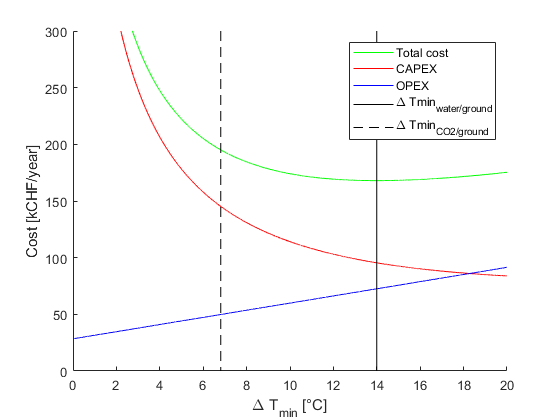
\includegraphics[width=0.7\linewidth]{dtmin_gtw}
	\caption{Optimization of $\Delta T_{min}$ values for heat exchange with the ground, through minimization of total costs (green line)}
	\label{fig:dtmin_gtw}
\end{figure}

%\begin{figure}[!htb]
%	\centering
%	\begin{minipage}{.45\textwidth}
%		\centering
%		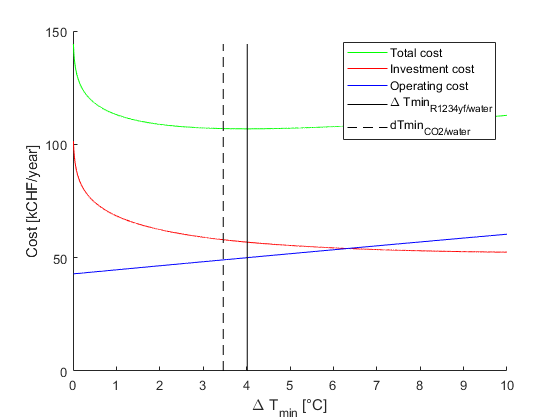
\includegraphics[width=\linewidth]{dtmin_wr}
%		\caption{Optimization of $\Delta T_{min}$ values for heat exchange with refrigerant R1234yf, through minimization of total costs (green line)}
%		\label{fig:dtmin_wr}
%	\end{minipage}%
%	\hspace{1cm}
%	\begin{minipage}{0.45\textwidth}
%		\centering
%		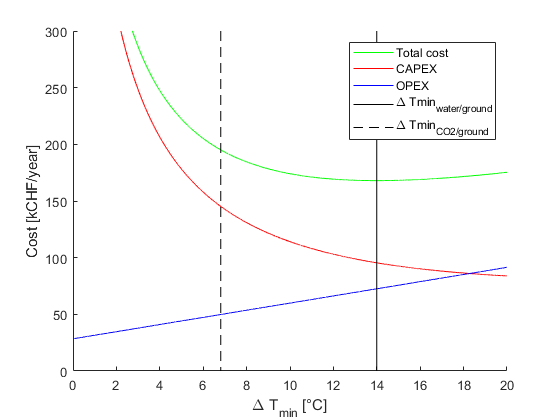
\includegraphics[width=\linewidth]{dtmin_gtw}
%		\caption{Optimization of $\Delta T_{min}$ values for heat exchange with the ground, through minimization of total costs (green line)}
%		\label{fig:dtmin_gtw}
%	\end{minipage}
%\end{figure}

\subsubsection{Compressor efficiencies}
The compressor efficiencies are directly calculated in the model, according to the equations in Section~\ref{sss:hp_CO2} and~\ref{sss:hp_thermo} in function of $P_{d}$ and $P_{s}$, respectively the pressure of discharge and suction of the compressor. Table~\ref{tab:eta_comp} shows the resulting efficiencies of the different heat pumps used in this work, for the average day in January.

\begin{table}[h!]
	\centering
	\caption{Calculated efficiencies for heat pump compressors, during the average day in January}\vspace{2mm}
	\label{tab:eta_comp} 
\begin{tabular}{l@{\hskip 0.5in}lllll@{\hskip 0.5in}lll} \toprule
	-             & \multicolumn{5}{c}{CO2 DEN}            & \multicolumn{3}{c}{Reference scenario} \\
	Unit          & CP     & CP   & SH     & DHW  & REF    & SH           & DHW       & REF         \\
	Refrigerant   & R123yf & CO2  & R123yf & R744 & R123yf & R123yf       & R744      & R123yf      \\ \midrule
	$P_{d}$       & 5.0    & 43.0 & 9.4    & 84.9 & 5.0    & 9.4          & 66.0      & 11          \\
	$P_{s}$       & 2.4    & 20.2 & 4.6    & 46.7 & 2.80   & 2.4          & 30.4      & 2.4         \\
	$\eta_{mech}$ & 0.85   & 0.80 & 0.85   & 0.78 & 0.85   & 0.85         & 0.80      & 0.85        \\
	$\eta_{is}$   & 0.85   & 0.70 & 0.85   & 0.71 & 0.85   & 0.82         & 0.70      & 0.81        \\
	$\eta_{comp}$ & 0.72   & 0.56 & 0.72   & 0.55 & 0.72   & 0.70         & 0.56      & 0.69       \\ \bottomrule
\end{tabular}
\end{table}

These values are similar to reference values found by Yang et al.\cite{yangTheoreticalExperimentalInvestigation2016} in their experimental work.


%\subsection{Analysis/Extrapolation scenario}
%A scenario to study parameters independently from Eglantine.
%Parameters to study/extrapolate for quick application on other districts:
%\begin{itemize}
%    \item influence on IC,OC,TC
%    \item influence on network temperature $T_net$  
%\end{itemize}
%Varying \% of cooling load, wrt heating load, using varying composition of cities, with categories (commercial/residential/...)


\subsubsection{Direct expansion HP}\label{sss:DX}
As discussed in Section~\ref{ss:dx}, there is the possibility to directly expand the CO2 into the geothermal well, instead of exchanging with help of a secondary water loop. To grasp the increase in performance, a simulation is performed on the CP of the CO2DEN technology. The used parameters, refrigerants and temperatures are shown in Table~\ref{tab:dxVSsl}. The CO2 heat pump has lower compressor efficiencies (see Table~\ref{tab:eta_comp}), which results in a lower $\eta_{COP}$. However it has a much lower temperature difference to cover, thanks to the direct expansion of the CO2, achieving a much higher COP value.

\begin{table}[htp]
\centering
\caption{Comparison of simulation results for a SL-GSHP, versus a DX-GSHP}\vspace{2mm}
\label{tab:dxVSsl} 
\begin{tabular}{lll}
	\toprule
	-                 & \begin{tabular}[c]{@{}l@{}}SL-GSHP\\ R1234yf\end{tabular} & \begin{tabular}[c]{@{}l@{}}DX-GSHP\\ R744\end{tabular} \\ \midrule
	$T_{source}^{lm}$ & 13                                                        & 13                                                     \\
	$T_{demand}^{lm}$ & 14                                                        & 14                                                     \\
	$T_{cond}^{lm}$   & 16.4                                                      & 15.8                                                   \\
	$T_{evap}^{lm}$   & -7                                                        & 8.2                                                    \\
	$COP_{real}$      & 6.5                                                       & 15.8                                                   \\
	$\eta_{COP}$   & ?                                  	                      & ?	                                                    \\
	$\eta_{exergy}$    & ?                                                         & ?   \\ \bottomrule                                                  
\end{tabular}
\end{table}


\subsubsection{Recalculation of the COP efficiency}
Running the optimization using heat pump models based on the thermodynamic cycle (see Section~\ref{sss:hp_thermo}) provides a very accurate results, but requires time consuming calculations. Depending on the application - for example for rough estimations at the beginning - it can be interesting to use the simplified model based on the carnot cycle instead (see Section~\ref{sss:hp_carnot}). Thus, it is found useful to recalculate the COP efficiency $\eta_{COP}$ values for all the concerned heat pumps, with respect to the operating conditions needed in this work. The calculation is straightforward, with the following equation:
\begin{equation}
\eta_{COP} = \frac{COP_{real}}{COP_{theoretical}}
\end{equation}

\begin{table}[h!]
\centering
\caption{Recalculated $\eta_{COP}$ values, with its operating temperatures}\vspace{2mm}
\label{tab:eta_COP_new} 
\begin{tabular}{lrrrrrrrr} \toprule
	& \multicolumn{5}{c}{CO2 DEN} & \multicolumn{3}{c}{Reference scenario} \\
	Unit & CP & CP & SH & DHW & REF & SH & DHW & REF \\ \midrule
	Refrigerant & R123yf & CO2 & R123yf & R744 & R123yf & R123yf & R744 & R123yf \\
$	T_{h}$ & 16.5 & 15.8 & 39 & 37.1 & 16.5 & 39.8 & 41 & 28.7 \\
$	T_{c} $& -9.4 & 5.2 & 11.5 & 11.5 & 2 & -5 & 5 & 2 \\
	$\eta_{COP}$ & 0.65 & 0.6 & 0.693 & 0.512 & 0.624 & 0.688 & 0.708 & 0.56 \\ \bottomrule
\end{tabular}
\end{table}

The new values are shown in Figure~\ref{tab:eta_COP_new}.

\clearpage
\newpage
\section{Results and discussion}

\subsection{Energy and exergy performance}\label{ss:perf}
%\todo{read through the section again}
A direct way to compare the performance of the different conversion technologies is the coefficient of performance, which is simply given by the ratio between the delivered heat $Q$ and the consumed electricity $E$. The \textit{heating}, \textit{cooling} and \textit{global} COP values are calculated in the following way:

\begin{align}
& COP_{heating} = \frac{Q_{SH}+ Q_{DHW}}{E_{SH} + E_{DHW} + E_{CP,winter}} \\
& COP_{cooling} = \frac{Q_{REF} + Q_{AC}}{E_{REF} + E_{CP,summer}} \\
& COP_{global} = \frac{Q_{SH}+ Q_{DHW} + Q_{REF} + Q_{AC}}{E_{SH} + E_{DHW} + E_{REF} + E_{CP,tot}}
\end{align}

where $E_{CP} = 0$ for the GS-HP. 

The COP values, calculated in each time step, are shown in Figure~\ref{fig:v_cop}. If the temperatures of evaporation and condensation of a heat pump are fixed, the operating cycle is also fixed, and thus the COP value. However, this is not always the case, as in certain cases the temperature of the energy demand (space heating) or of the heat source/sink (soil, air, water...) varies in function of time. In this case, a fixed condensation temperature would imply high exergy losses, given that most of the time the approach temperature would be larger than the minimum required one. Modern HP can therefore adapt their operating cycle in order to fit the varying heat demand temperature. This results in non-constant COP value, as it can be seen for the SH HP (blue line), which varies between 6 and 14. The same happens to the refrigeration system in the GS-HP that perform worse during summer, when they have to deliver heat to a higher ambient temperature. In comparison, the COP of refrigeration in the CO2DEN are constant, since heat is delivered at a constant temperature throughout the year to the CO2 network.

\begin{figure}[tph]
	\centering
	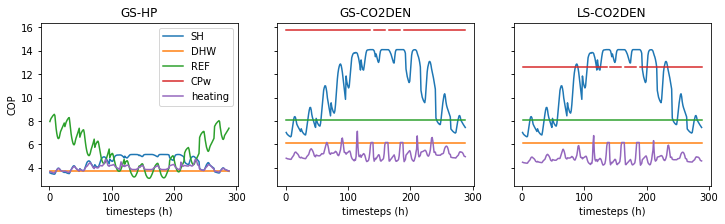
\includegraphics[width=1\linewidth]{Images/V_COP}
	\caption{Comparison of COP values for each time step t and unit. The \textit{cooling } and the \textit{global} COP are not displayed given the different order of magnitude due to the free cooling}
	\label{fig:v_cop}
\end{figure}

The COP for the heating heat pumps SH and DHW are considerably higher in the CO2DEN. This is due to the "two stages" of the conversion technology: the heat is first furnished to the CO2 network by the CP and then brought up to the required temperature by the decentralized HP. Thus to consider the resulting COP for heating facilities, the values from the CP, SH and DHW would have to be combined. The COP of the central plant is higher in the GS CO2DEN, being the evaporation temperature higher than in the heat exchange with the lake. 

\begin{table}[htp]
\centering
\caption{COP values for the three energy system}\vspace{2mm}
\label{tab:V_cops} 
\begin{tabular}{lrrr}
	\toprule
	& GS-HP & GS-CO2DEN & LS-CO2DEN \\ \midrule
	HP-SH            & 4.5  & 10.8    & 10.8    \\
	HP-DHW           & 3.8  & 6.2     & 6.2     \\
	HP-REF           & 5.4  & 8.1     & 8.1     \\
	HP-$CP_{winter}$ & -    & 15.8    & 12.6    \\
	Heating          & 4.0  & 5.2     & 4.9     \\
	Cooling          & 19.1 & 50.4      & 50.4      \\
	Global           & 4.6  & 6.1     & 5.6    \\ \bottomrule
\end{tabular}
\end{table}


The mean COP values for each technology are shown in Table~\ref{tab:V_cops}. The GS-CO2DEN shows the best performance with a global COP of 6.1. The LS-CO2DEN follows with 5.6 and the GS-HP with 4.6. The increase in the global COP is reflected in a reduced electricity consumption by the energy system; this is shown in Table~\ref{tab:V_el}. With respect to the GS-HP, the GS-CO2DEN requires 24\% and the LS-CO2DEN 17\% less electricity.\\

\begin{table}[htp]
\centering
\caption{Electricity consumption of the three energy conversion technologies}\vspace{2mm}
\label{tab:V_el} 
\begin{tabular}{lrrr}
	\toprule
	& GS-HP & GS-CO2DEN & LS-CO2DEN \\ \midrule
	Electricity consumption & & & \\
	Corresponding reduction & - & 24\% &  17\% \\
	\bottomrule
\end{tabular}
\end{table}


The exergy values of supply and demand have been calculated for each conversion technology, as explained in Section~\ref{ss:exergy}. This analysis shows the real thermodynamic value of the required energy services, since not only the amount of heat is considered, but also the temperature level at which it happens. The exergy value of the demand is thus calculated in function of the varying ambient temperature and is the same for all technologies.

The exergy efficiency for the different energy conversion technologies are shown in Table~\ref{tab:V_exergy}. It is clear to see that the GS-HP performs worse than the CO2 technologies with 24\%, against 32\% of the GS-CO2DEN and 30\% of the LS-CO2DEN. This difference is explained by the lower exergy efficiency of the GS-HP, which presents higher minimum approach temperatures, as well as a lower COP of the heat pumps. The reason for the high performance of the GS-CO2DEN, despite having two stages and thus some additional losses due to $\Delta T_{min}$ values, is the direct expansion of CO2. As shown in Section~\ref{sss:DX}, the energy and exergy gain, with respect to the conventional system based on a secondary water loop, are important.

\begin{table}[htp]
\centering
\caption{Comparison of the exergy losses $\dot{L}$ and efficiencies $\eta_{exergy}$, with and without considering renewable PV production}\vspace{2mm}
\label{tab:V_exergy} 
\begin{tabular}{llrrr} \toprule
	-                    & units & GS-HP & GS-CO2DEN & LS-CO2DEN \\ \midrule
	$\dot{L}_{\Delta T_{min}}$       & [MWh] & 77    & 47        & 47        \\
	$\dot{L}_{HP}$             & [MWh] & 355   & 242       & 281       \\
	$\dot{L}_{tot}$            & [MWh] & 432   & 289       & 327       \\
	$\eta_{exergy}$      & [\%]  & 17\%   & 22\%       & 21\%       \\
	$\eta_{exergy}^{PV}$ & [\%]  & 27\%   & 35\%       & 33\%      \\ \bottomrule
	\end{tabular}
\end{table}


Figure~\ref{fig:v_exe} shows the exergy efficiency for the different conversion technologies, calculated for each time-step - the values are sorted in decreasing order. It can be seen that the exergy efficiency is dependent from the operating temperatures, as well as from the ambient temperature. Thus the exergy efficiencies vary between 10-50\% throughout the year. Moreover, the graph shows that the quality of the energy system, i.e. the order of best and worst performing technologies, remains the same during all time steps.

\begin{figure}[tph]
	\centering
	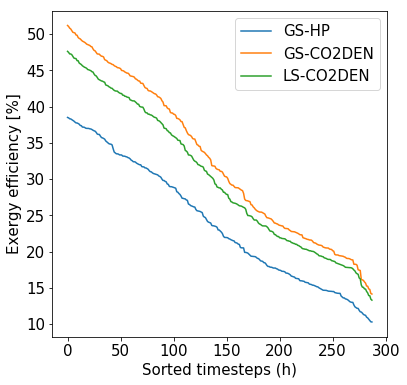
\includegraphics[width=0.45\linewidth]{exe}
	\caption{Exergy efficiencies calculated in each time step - sorted in decreasing order}
	\label{fig:v_exe}
\end{figure}

\subsection{Financial analysis}
A financial analysis of the three conversion technologies is shown in Figure~\ref{fig:V_costs}. 
The used cost functions, energy prices and maximal available PV area are given in Table~\ref{tab:cc}. \\

\begin{table}[htp]
	\centering
	\caption{Summary of relevant cost and decision constraints.}
	\label{tab:cc}
	\begin{tabular}{ll}
		\toprule
		Cost functions         & Table~\ref{tab:ic} in Section~\ref{sss:cf}         \\
		Electricity cost       & Table~\ref{tab:ec} in Section~\ref{sss:cf}       \\
		Max. PV area available & 2170 $m^2$ (see Table~\ref{tab:pv} in Section~\ref{ss:pv})\\ 
		\bottomrule
	\end{tabular}
\end{table}

Given that in this work the cost of operation (OC) depends only from the consumed electricity (no consumption of gas or other resources), this is directly correlated to the global COP of the system. As seen above (see Table~\ref{tab:V_cops}), GS-CO2DEN presents the highest coefficient of performance and thus also the lowest OC (dashed line), with $260'000[Euro/yr]$, and GS-HP the highest with $290'000[Euro/yr]$. The LS-CO2DEN presents an OC of $270'000[Euro/yr]$.\\

The investment costs (IC) are shown more in detail in the clustered columns. It is easy to note that the GS-HP has much lower upfront costs ($180'000[Euro/yr]$) than the GS-CO2DEN solution ($220'000[Euro/yr]$). Indeed, due to the higher COP values, a larger share of heat comes from the geothermal wells, which increases their investment cost. Moreover, there is the additional cost of the CO2 pipes needed to connect all the user. In the SL-CO2DEN there are obviously no costs related to the geothermal wells, but the cost for the water pipes that allow the water to be brought to the CP. Given the actual distance of the Eglantine district from the lake, this solution leads to much higher upfront costs than the competing technologies ($310'000[Euro/yr]$).\\

Despite the lower OC for the CO2DEN technologies, the total cost (TC) is clearly following the tendency of the IC, which present a larger difference. The GS-HP ends up being the cheapest variant with $470'000 [Euro/yr]$, followed by the GS-CO2DEN with an only slightly higher cost of $485'000 [Euro/yr]$. The SL-CO2DEN is the most expensive solution with $580'000 [Euro/yr]$.\\

Self consumption and autarchy do not vary much between the technologies, because no storage technology has been taken into account. Indeed, any kind of storage - thermal, electrical or CO2 - would help to adapt the energy consumption in order to increase the self-consumption, as well as to reduce peak demands. Moreover, despite of the optimizer choosing to install the maximum possible amount of PV for all technologies, in order to reduce the OC, the amount of electricity produced is seldom larger than the total electricity demand of the district. Thus, the three systems have an autarchy of about 25\%, and a self consumption rate of around 95\%.\\

For what has been seen in this section, the CO2 network showed an good energy performance. However, the reasons to opt for such a technology will have to go beyond financial arguments, since it remains a more expensive solution, even it this could quickly change if the price of electricity rises, which is not such a far-fetched scenario. Another strong argument in favor of this technology is the space planning. A city center might first of all not have the space for, but also not want everyone to drill boreholes under its house. The CO2 network would allow to profit from its benefits, while outsourcing and give flexibility to the planning and realization of the geothermal field.

\begin{figure}[htp]
	\centering
	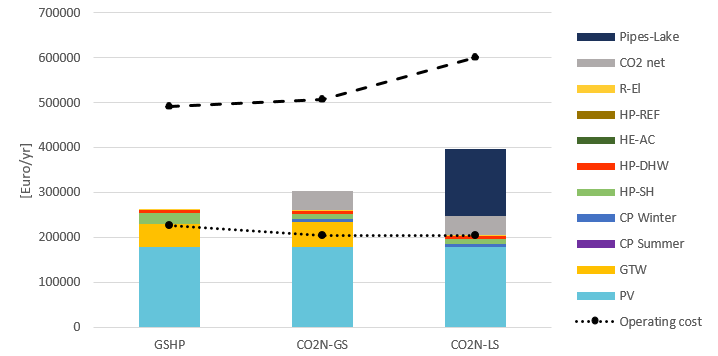
\includegraphics[width=1\textwidth]{V_costs.PNG}
	\caption{Cost comparison for the three different energy systems variants}
	\label{fig:V_costs}
\end{figure}


\subsubsection{Parametric optimization of GS-HP}
A parametric optimization of the costs of the reference energy system (GS-HP) is shown in Figure~\ref{fig:V_G_PO}. The optimizer is let to optimize the operating costs, while step-wise constraining the investment cost. This is a help for decision making. The used cost functions, energy prices and maximal available PV area are given in Table~\ref{tab:cc}. \\ 

\begin{table}[htp]
	\centering
	\caption{Summary of relevant cost and decision constraints.}
	\label{tab:cc_sa}
	\begin{tabular}{ll}
		\toprule
		Cost functions         & Table~\ref{tab:ic} in Section~\ref{sss:cf}         \\
		Electricity cost       & Table~\ref{tab:ec} in Section~\ref{sss:cf}       \\
		Max. PV area available & 4340 $m^2$ (see Table~\ref{tab:pv} in Section~\ref{ss:pv})\\ 
		\bottomrule
	\end{tabular}
\end{table}

It can be seen that the biggest difference in investment and operating cost is due to the sizing of the PV - for which an increased area is considered in this case (see Table~\ref{tab:cc_sa}), accounting for potential facades and free space PV. When constraining the investment costs, the model installs only a small share of PV, which increases the operational costs. On the contrary, a high share of PV increases the systems rate of auto-sufficiency, lowering the operational costs. 

By lowering the constraint on the IC (towards the right side of the graph), the maximum allowed share of photovoltaic (PV) is reached. However, the operational are additionally lowered thanks to a different handling of peak consumption. The optimal system installs a small share of electrical heater (R-EL) to cover peak demand, which allows to optimally size the heating heat pumps (HP-SH, HP-DHW). In the last column on the right, the system chose not to install the electrical heater but installing larger heat pumps, which strongly increases upfront costs, but allows to further reduce the operational costs.

By increasing the constraint on the IC (towards the left side of the graph), the opposite phenomenon happens, i.e. no PV are installed to reduce the investment costs. To further reduce upfront costs, the system chose to cover the heat demand almost entirely with help of the electric heater, minimizing the size of the heating heat pumps.

The optimum with respect to the total cost of the energy system, located somewhere in the middle of the graph, is analyzed in the following chapters.

\begin{figure}[htp]
	\centering
	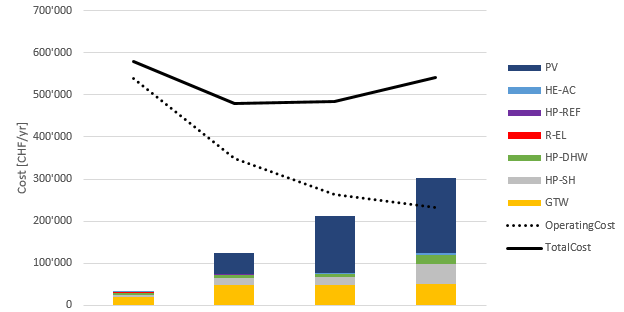
\includegraphics[width=1\textwidth]{V_G_PO1.png}
	\caption{Parametric optimization of the reference energy system (GS-HP), showing the detailed investment costs, the operational cost and the total cost.}
	\label{fig:V_G_PO}
\end{figure}

\subsubsection{Parametric optimization of GS-CO2DEN}
A parametric optimization of the costs of the CO2 district energy system with ground sourced central plant (GS-CO2DEN) is shown in Figure~\ref{fig:V_CO2_G_PO}. The optimizer is let to optimize the operating costs, while step-wise constraining the investment cost. This is a help for decision making. The used cost functions, energy prices and maximal available PV area are given in Table~\ref{tab:cc}. \\ 

The response of this system to the parametric optimization is very similar to the one of the GS-HP system. This means that the biggest difference in investment and operating cost is due to the sizing of the PV - for which an increased area is considered also in this case (see Table~\ref{tab:cc_sa}) -, while the extreme cases are determined by the ratio between the electrical heater and the heating heat pumps. The optimum is analyzed in the following chapters.\\

\begin{figure}[htp]
	\centering
	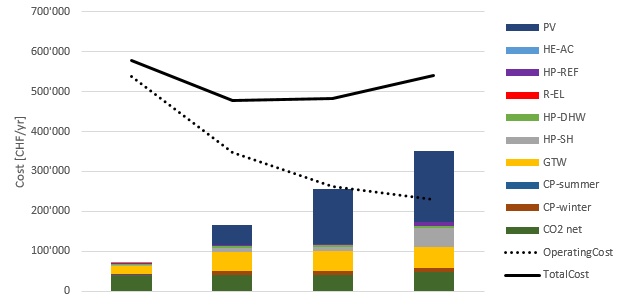
\includegraphics[width=1\textwidth]{V_CO2_G_PO1.png}
	\caption{Parametric optimization of the ground sourced CO2 DEN (GS-CO2DEN), showing the detailed investment costs, the operational cost and the total cost}
	\label{fig:V_CO2_G_PO}
\end{figure}

In order to discuss the validity of the results, the investment costs have been benchmarked against two other existing anergy networks in Switzerland - the \textit{Anergienetz ETH Hönggerberg }and the \textit{Anergienetz Friesenberg}. This is done by comparing the share of the total cost represented by the network, the geothermal wells and the heating and cooling facilities. The resulting percentages are shown in Table~\ref{tab:anergynets_IC}. It can be seen that the GS-CO2DEN system in the Eglantine district presents a much lower percentage of the investment cost  $IC_{Heating/cooling}$ attributed to the heating and cooling equipment (HP-SH, HP-DHW, HP-REF, HE-AC), with respect to the other two networks. This leads to higher shares of investment costs attributed to the CO2 network and the geothermal field.

\begin{table}[h!]
\centering
\caption{Cost comparison with existing anergy systems}\vspace{2mm}
\label{tab:anergynets_IC} 
\begin{tabular}{llrrr}  \toprule
	&          & Eglantine & \begin{tabular}[c]{@{}l@{}}Anergienetz \\ ETH Hönggerberg\end{tabular} & \begin{tabular}[c]{@{}l@{}}Anergienetz \\ Friesenberg\end{tabular} \\ \midrule
	$IC_{NET}$             & [\%]     & 33.6 \%    & 15.7 \%                                                                 & 25.9 \%                                                             \\
	$IC_{GTW}$             & [\%]     & 44.6 \%    & 32.7 \%                                                                 & 23.5 \%                                                             \\
	$IC_{Heating/Cooling}$ & [\%]     & 21.8 \%    & 49.2 \%                                                                 & 50.6 \%                                                             \\
	Heating power          & [kW]     & 592       & 8'000                                                                  & 3'930                                                              \\
	Heating demand         & [MWh/yr] & 2'390     & 28'450                                                                 & 35'000                                                             \\
	Cooling power          & [kW]     & 84        & 6'000                                                                  & 3'500                                                              \\
	Cooling demand         & [MWh/yr] & 33        & 26'200                                                                 & 80'000                                                             \\ \bottomrule
%	Tot. Cost (excl. PV)   & [mioCHF] & 1.65      & 37                                                                     & 43                                                                
\end{tabular}
\end{table}

One reason for this difference is most likely the size difference between the energy systems. In fact, the Eglantine system is drastically smaller than the one at ETH or in Friesenberg, which have a heating demand which is respectively 12 and 15 times bigger. The specific investment costs for building the network and drilling the geothermal wells decreases with size - for example the costs of digging to place a pipe underground won't be strongly correlated with the pipe diameter. On the contrary, the specific costs for the heat pumps will stay about the same, given that the size of the decentralized heat pumps will not increase, only its number.

On the other hand, it is not trivial to estimate the cost of building the CO2 network, given the lack of real applications, and the resulting costs could be proven to be inaccurate. Also the sizing of the geothermal well, in order to account for yearly energy balance and recharge rate, and for the specific cost, according to depth and soil type would have to be verified and confirmed through further studies and simulations.


\subsection{Heat source integration}

\begin{figure}[thpb]
	\centering
	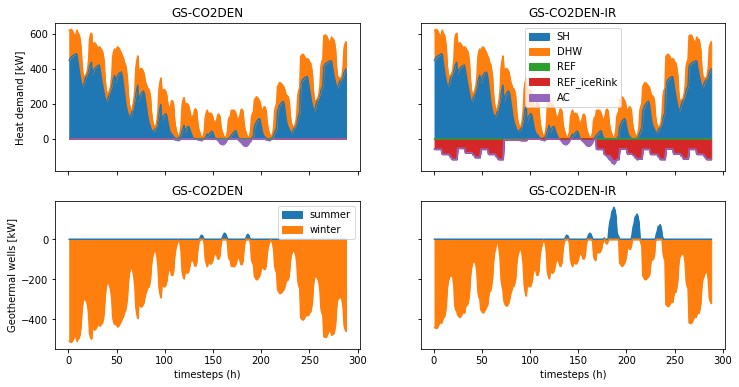
\includegraphics[width=1\linewidth]{Images/V_IR_Q}
	\caption{Comparison of the heating (+) / cooling (-) demand - upper row - and the heat extracted (+) / injected (-) into the boreholes - lower row - before - left column - and after - right column - integration of the ice rink}
	\label{fig:V_IR_Q}
\end{figure}


The integration of large external heat sources, as for example an ice rink, is very interesting for a CO2 district energy network, since heat recovery allows to reduce the load of the CP, and thus the load of the heat source. It has been assumed that the existing facility already exists, and therefore its energy demands are not included in the model. This means that also the gain in performance of the cooling system, through the lower condensation temperature obtained by exchanging with the CO2 network, is not taken into account. The external heat source is purely considered as a free heat source. The used cost functions, energy prices and maximal available PV area are given in Table~\ref{tab:cc}. \\ 

Figure~\ref{fig:V_IR_Q} shows the heat demand of the system (upper row) and the heat exchange with the heat source (lower row), by comparing the system before (left column) and after (right column) the integration of the ice rink. The additional cooling demand of the ice rink is shown in red. The increased cooling demand reduces the amount of heat that has to be furnished by the CP, thus reducing the total energy demand of the system - the global COP raises from 6.12 to 6.73. This also means that less heat will be extracted from the geothermal wells: this is reflected in the reduction of the orange area in the lower row, which corresponds to the amount of heat that is extracted from the source, throughout the year.


An analysis of the economic differences caused by the integration of the ice rink is shown in Figure~\ref{fig:V_IR_cost}. The reduced use of the CP lowers the electricity demand of the heating/cooling facility from $470'000$ to $435'000 [kWh/yr]$ - which corresponds to a reduction of 9\%. At the same time, the lower peak use of the GTW reduces its IC. On the other hand, the integration of the external heat source requires the installation of additional CO2 pipes, which has an impact on the upfront costs. The resulting difference in the total cost is negative, i.e. the total cost of the CO2 energy network is lower if the ice rink is connected, by about 4'000 [Euro/yr]. This is not yet sufficient to have a lower cost than the GS-HP, but its reducing the gap to about 10'000 [Euro/yr]. Note that, as mentioned before, the reduction in operating costs in the ice rink cooling facility, which would strongly increase the energy and economic gain of the heat source integration, has not been taken into account.\\

%\begin{figure}[tph]
%	\centering
%	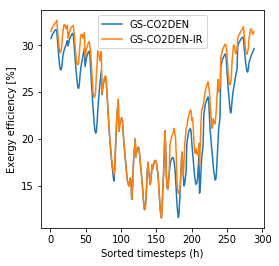
\includegraphics[width=0.45\linewidth]{Images/V_IR_exe}
%	\caption{Comparison of exergy values of the GS-CO2DEN technology with and without the integration of the ice rink (IR)}
%	\label{fig:virexe}
%\end{figure}
%
%From an exergy point of view, the integration of the external heat source replaces a share of the exergy value of the electricity. This translates in a higher exergy efficiency for those time steps in which the external heat source is available, as shown in Figure~\ref{fig:virexe}. The mean exergy efficiency increases from 22.4\% to 23.7\%.

\begin{figure}[tph]
	\centering
	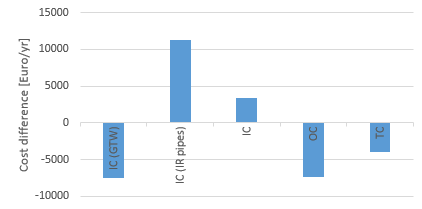
\includegraphics[width=0.7\linewidth]{Images/V_IR_cost}
	\caption{Cost difference of the GS-CO2DEN with and without ice rink. Positive values (+) reflect a higher, and negative values (-) a lower cost originated by the IR integration.}
	\label{fig:V_IR_cost}
\end{figure}


\begin{figure}[tph]
	\centering
	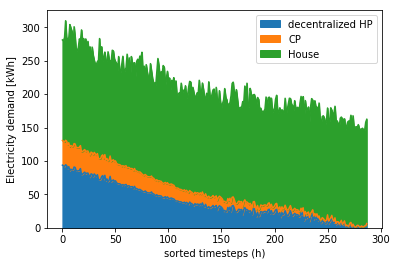
\includegraphics[width=0.7\linewidth]{Images/V_CO2_eldem_sorted}
	\caption{Electricity demand of GS-CO2DEN system grouped in categories, sorted in decreasing order}
	\label{fig:gsco2_el}
\end{figure}

Figure~\ref{fig:gsco2_el} shows the shares of electricity consumption, on a sorted time axis. What is interesting to note is the shares of electricity consumption between the CP and the decentralized HP. $E_{cp}$ represents around 10\% of the global electricity consumption, and around 30\% of the $E_{heat/cool}$. This means that even a system having a perfectly balanced heating and cooling demand would not be able to reduce its OC of more than 30\%, since, as far as the temperature of the CO2 network remains constant, the operating conditions of the decentralized heat pumps remain unchanged too.\\

Furthermore, it is important to account for uncertainties bound to the external heat source. For example for an ice rink, the replacement of the obsolete and inefficient cooling facility, or an improvement in the facility management, can drastically reduce its energy. Same for other potential heat sources as industrial processes, which can be improved or replaced over time. This should be considered in the inclusion of external heat source, since a reduction, or the absence, of the additional heat could threaten the functioning of the system.


\subsection{Ground temperature response}\label{ss:Tg}

%\begin{figure}[htp]
%	\centering
%	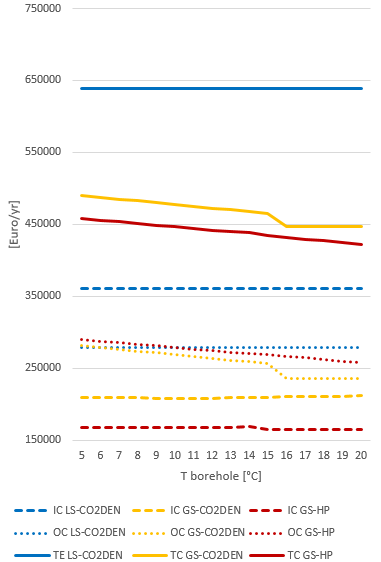
\includegraphics[width=0.45\textwidth]{V_SA_Tg.png}
%	\caption{Cost comparison of variants in function of the borehole temperature}
%	\label{fig:V_SA_Tg}
%\end{figure}
%\todo{wrapfigure}

\begin{wrapfigure}{R}{0.6\textwidth} 
	\vspace{-20pt}
	\centering
	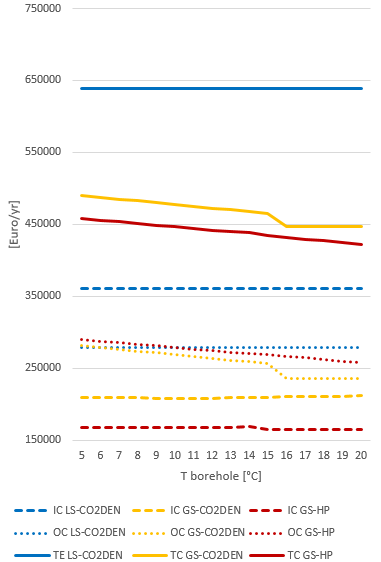
\includegraphics[width=0.58\textwidth]{V_SA_Tg.png}
	\caption{Cost comparison of variants in function of the borehole temperature. The gray area represents the geothermal depth - in the Lemanic region - that corresponds to a given temperature}
	\label{fig:V_SA_Tg}
	\vspace{-10pt}
\end{wrapfigure}

A critical parameter for the efficiency of a ground sourced energy system is the ground temperature. As seen in Section~\ref{ss:gtw}, this temperature depends mainly on the depth, the temperature gradient in the given soil and the surface temperature. In other words, it is dependent from the location - including local climate and altitude - and the depth of drilling. In order to acknowledge the influence this temperature has on the system's performance, a sensitivity analysis has been performed. The results are shown in Figure~\ref{fig:V_SA_Tg}. The used cost functions, energy prices and maximal available PV area are given in Table~\ref{tab:cc}. \\ 

The GS-HP energy system seems to responds in a linear way to the temperature raise, as it can be expected, thanks to the lower required temperature raise for heating, which increases the COP of the system. In reality a small step can be identified between 14 and 15 \si{\celsius}, at which the IC drop and the OC rise. This step happens when the ground is not cool enough anymore to offer the option of free-cooling. The system is forced to use a refrigeration system instead, which increases the OC. However this utility is already installed, and thus the increase of $IC_{HP-REF}$ is lower than the reduction of the obsolete $IC_{HE-AC}$.

The GS-CO2DEN energy system presents a more evident step in its response to the ground temperature. The reason lies in the use of the central plant, which, as described in Section~\ref{sss:CO2DEN}, has different operating modes for cooling and heating. In fact, if the temperatures are either high or low enough, it can operate free-cooling or free-heating. In any other case, it operates in cooling and/or heating HP mode. In this case the step happens at $T_{b} \geq 16 \si{\celsius}$, for which the CP can source heat directly from the ground without the need of a heat pump, which drastically reduces the operational costs.

Assuming uniform soil and maintaining a constant heat capacity, a higher borehole temperature would imply drilling a smaller number of wells with greater depth. In other words, the geothermal model described in Section~\ref{ss:gtw} simply models the heat capacity and the investment cost per borehole meter. It is thus not able to properly account for advanced correlations between heat capacity, cost function and well depth. Moreover the regeneration rate of the soil should be consider, in order to properly model its temperature, in function of the heat extracted throughout days, seasons and years.

Nevertheless, this sensitivity analysis gives an idea of the global behavior response of the different conversion technologies to the ground temperature. This can be very helpful to estimate the performance of either system, in function of the geographical location, latitude and altitude.


\subsection{Lake distance}

%
%For obvious reason, while GS-CO2DEN and GSHP respond similarly to the variation in the bore temperature, the LS-CO2DEN presents constant costs. In fact the system is not dependent from the ground temperature and is represented on the graph for sake of comparison. It can be seen that $OC_{LS-CO2DEN}$ performs better, in terms of operating costs, than the GS-HP at any ground temperature in the studied interval. It also performs better than the GS-CO2DEN for temperatures below 10 \si{\celsius}. The lake distance in the Eglantine district is 1500m , which results in very high investment costs, precluding the competitiveness of this solution, in the given conditions.\\ 

\begin{wrapfigure}{R}{0.5\textwidth} 
	\vspace{-20pt}
	\centering
	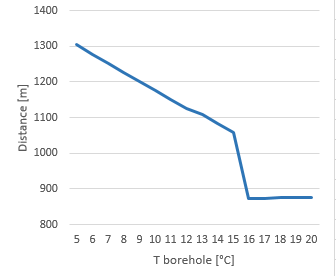
\includegraphics[width=0.45\textwidth]{lakeDist.png}
	\caption{Maximum distance of lake for which $TC_{LS-CO2DEN}$ is lower than $TC_{GS-CO2DEN}$ (blue) and $TC_{GS-HP}$ (yellow), in function of the ground temperature $T_{borehole}$. The dashed vertical line shows the values corresp. to the case study ground temperature.}
	\label{fig:lakeDist}
	\vspace{-23pt}
\end{wrapfigure}

As it has been seen in the Section~\ref{ss:perf}, the LS-CO2DEN presents competitive OC. However its investment costs strongly depend on the necessary pipe length. Therefore, there will be a distance under which the LS-CO2DEN presents a lower total cost than the concurrent systems. This threshold distance depends on the ground temperature, given that the TC of the GS-HP and the GS-CO2DEN vary accordingly. The resulting thresholds are plotted on Figure~\ref{fig:lakeDist}. This helps choosing between using the lake or the soil as a heat source, knowing the mean ground temperature and the distance from the lake water.

%\begin{figure}[htp]
%	\centering
%	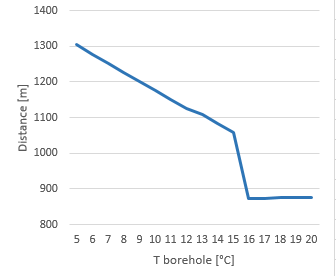
\includegraphics[width=0.4\textwidth]{lakeDist.png}
%	\caption{Maximum distance of lake for which the total costs are lower than the two other energy systems, in function of the ground temperature $T_{borehole}$}
%	\label{fig:lakeDist}
%\end{figure}
%\todo{wrapfig}

At $T_{borehole} = 12 \si{\celsius}$, as in the Eglantine district, the LS-CO2DEN would be a financially interesting solution against  GS-HP and GS-CO2DEN if the distance to the lake is respectively shorter than 328 and 484 meters.

The used cost functions, energy prices and maximal available PV area are given in Table~\ref{tab:cc}.

\newpage
\subsection{Optimization of energy demand}

The Eglantine district is composed for 97\% of buildings dedicated to residential use (see Section~\ref{ss:Eglantine}), resulting in a very low cooling and refrigeration demand. It is now legitimate to wonder how the different energy systems would perform in a different district, i.e. with a different building use and thus a differently composed energy demand. In this chapter, it will be tried to answer this question, finding out the optimum district composition for the performance of a GS-CO2DEN system. The used cost functions, energy prices and maximal available PV area are given in Table~\ref{tab:cc_cu}. It has to be noted that, in order to focus on the energy performance of the heating and cooling energy system, the electricity consumption of the houses has been neglected in this subsection.\\ 

\begin{table}[htp]
	\centering
	\caption{Summary of relevant cost and decision constraints.}
	\label{tab:cc_cu}
	\begin{tabular}{ll}
		\toprule
		Cost functions         & Table~\ref{tab:ic} in Section~\ref{sss:cf}         \\
		Electricity cost       & Table~\ref{tab:ec} in Section~\ref{sss:cf}       \\
		Max. PV area available & 2170 $m^2$ (see Table~\ref{tab:pv} in Section~\ref{ss:pv})\\
		Electricity consumption of houses	 & 0 \\ 
		\bottomrule
	\end{tabular}
\end{table}

The building categories (see Table~\ref{tab:ppa_buildinguse}) and its specific energy demand in $[kWh/m^2]$ are shown in Table~\ref{tab:specificE}.\\

\begin{table}[htp]
	\centering
	\caption{Specific annual energy demand per building use~\cite{girardinEnerGisGeographicalInformation2010}.}
	\label{tab:specificE}
	\begin{tabular}{llllll}
		\toprule
		Energy demand $[kWh/yr/m^2]$ & $q_{SH}$ & $q_{DHW}$ & $q_{AC}$ & $q_{REF}$ & $e_{el}$ \\ \midrule
		Housing & 30 & 21 & 0 & 0 & 28 \\
		Retail & 24 & 7 & 53 & 6.8 & 33 \\
		Restaurant services & 32 & 56 & 11 & 0 & 33 \\
		 \bottomrule
	\end{tabular}
\end{table}

For sake of simplicity, among the categories shown in Table~\ref{tab:ppa_buildinguse}, the two most common and diverse - i.e. presenting the most different energy demand - have been chosen: (1) Housing (H) and (2) Retail (R). \\

A sensitivity analysis has been performed on a district composed by those two categories. The energy demand resulting from the different combinations of the above mentioned categories is shown in Figure~\ref{fig:cu}. At the far right the energy demand resulting from a district composed by 100\% of retail buildings, with a decreasing share towards the left. More details about the total and the specific heating and cooling energy demand are given in Table~\ref{tab:CU_energy}. The last column on the left is given by the Eglantine district, as a reference. It is clear to see that the retail building has a high cooling demand during summer months, with demand peaks that are around 4 times the heating demand peaks. Moreover, while the space heating demand remains very similar, the hot water demand decreases considerably.

\begin{table}[h!]
\centering
\caption{Comparison of energy demand and energy performance of the different combination of building use}\vspace{2mm}
\label{tab:CU_energy} 
\begin{tabular}{llrrrrrrr} \toprule
                 &       & Eglantine & \begin{tabular}[c]{@{}l@{}}H1 / \\ R0\end{tabular} & \begin{tabular}[c]{@{}l@{}}H0.8 / \\ R0.2\end{tabular} & \begin{tabular}[c]{@{}l@{}}H0.6 /\\ R0.4\end{tabular} & \begin{tabular}[c]{@{}l@{}}H0.4 / \\ R0.6\end{tabular} & \begin{tabular}[c]{@{}l@{}}H0.6 / \\ R0.8\end{tabular} & \begin{tabular}[c]{@{}l@{}}H0 / \\ R1\end{tabular} \\ \midrule
	$Q_{heating}^{+}$ & [MWh] & 2'402     & 2'347   & 2'1614      & 1'976       & 1'790       & 1'603       & 1'426   \\
	$Q_{cooling}^{+}$ & [MWh] & 39        & 20      & 549         & 1'113       & 1'677       & 2'241       & 2'777   \\
	$Q_{GTW}^{netBalance}$ & [MWh] & -1'887    & -1'863  & -1'195      & -482        & 234'        & 951         & 1'632   \\
	$COP_{heating}$   & [-]   & 5.1       & 5.1     & 5.4         & 5.7         & 5.9         & 6.1         & 6.3     \\
	$COP_{cooling}$   & [-]   & 63.1      & 52.3    & 72.8        & 73.7        & 74.1        & 74.2        & 74.3    \\
	$COP_{global}$    & [-]   & 5.9       & 5.5     & 14.7        & 22.3        & 29.3        & 36.3        & 43.6   \\ \bottomrule
\end{tabular}
\end{table}

\begin{figure}[tph]
	\centering
	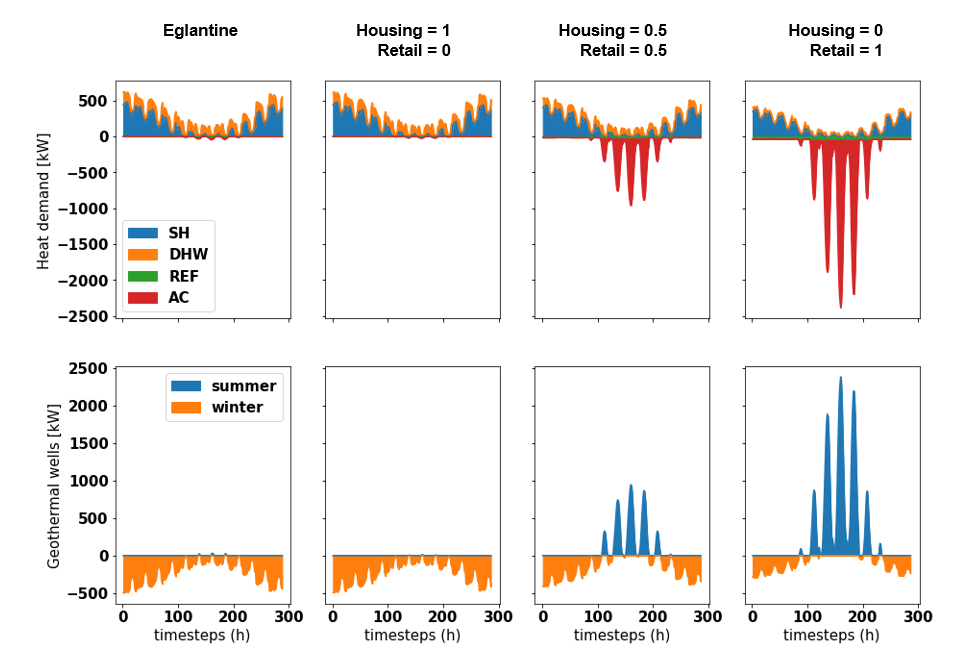
\includegraphics[width=1\linewidth]{Images/CU}
	\caption{Comparison of the heating (+) / cooling (-) demand - upper row - and the heat extracted (+) / injected (-) into the boreholes - lower row - for different district compositions.}
	\label{fig:cu}
\end{figure}

Table~\ref{tab:CU_energy} shows the COP values for the energy system throughout the different combinations of buildings use. The $COP_{heating}$ increase is due to the decreasing share of DHW, which is heated with a lower COP. The increase in cooling, and thus the strong increase in the global coefficient of performance is due to the fact that the biggest share of the cooling demand can be satisfied with free-cooling. These variations are reflected in the decrease of electricity consumption, shown in the upper row of Figure~\ref{fig:cu}. The resulting heat exchange with the geothermal wells is shown in the lower row of Figure~\ref{fig:cu}.

\begin{figure}[htp]
	\centering
	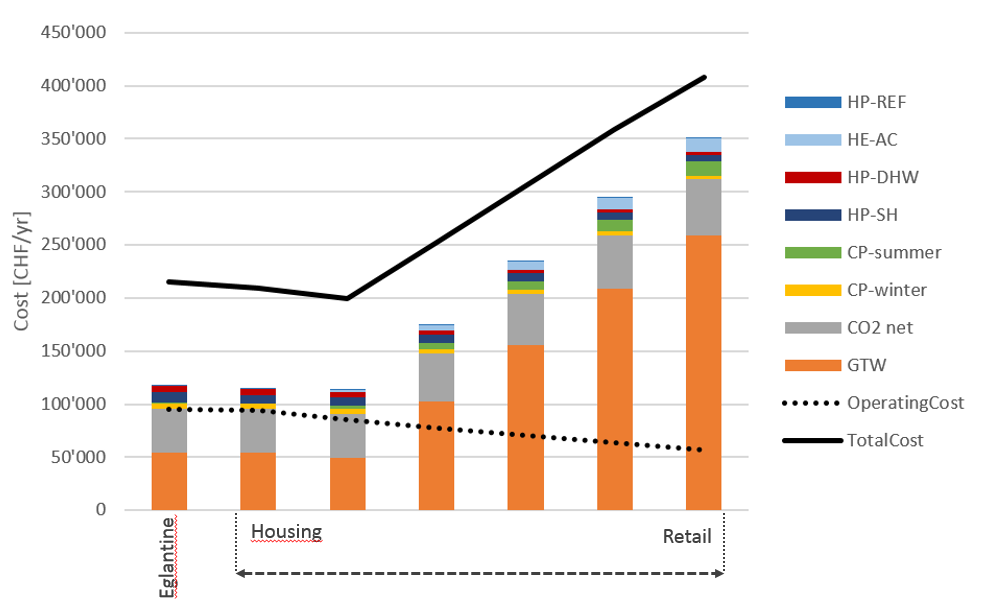
\includegraphics[width=1\textwidth]{CU_SA_TC.png}
	\caption{Cost comparison for different combinations of \textit{housing} and \textit{retail} building use, with the Eglantine district as a reference in the first column. The stacked columns show the investment costs.}
	\label{fig:CU_TC}
\end{figure}

\begin{figure}[tph]
	\centering
	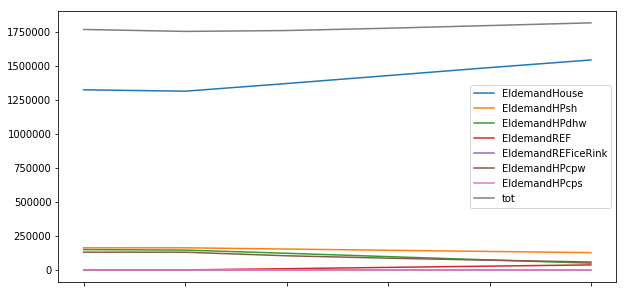
\includegraphics[width=0.55\linewidth]{Images/CU_el}
	\caption{Electricity demand in function of the building use composition}
	\label{fig:CU_el}
\end{figure}

Figure~\ref{fig:CU_TC} shows the resulting costs, for the different scenarios. The operating costs decrease linearly, with the increase of the share of retail use. This is due to the smaller heating demand. The increasing cooling demand is essentially satisfied with free-cooling, which does not influence the operating cost. This means that the optimum district composition, if only the operating costs are taken into account, is a purely retail based district.\\

However, the increasing amount of energy that has to be dissipated in the ground has a big impact on the investment cost, since the model sizes the GTW in order to satisfy the peak cooling power, which is around 2000 kW for a retail composed district. In comparison, the peak heating demand in the Eglantine district sums up to 500 kW. Therefore, the increase in the IC is much bigger than the decrease of OC. In theory, the amount of heat extracted and injected in the ground should also be taken into account in the sizing of the GTW. Indeed, the geothermal field can be used as a heat storage between the seasons. In Table~\ref{tab:CU_energy} the net heat balance over a year is shown for each combination of district use. Thus, the fact that the model in this work sizes the GTW exclusively on the peak demand, is probably resulting in an overestimation of the investment costs for the GTW.

The optimum combination of the district composition, in terms of total cost, is to be found in low shares of retail, where the cooling demand allows to partly compensate the heating demand - thus reducing the operation cost - without increasing the peak demand for the GTW. To find the precise value, a model that lets the solver choose the composition of the district has been implemented. This requires an additional set of constraints, which ensures that the chosen composition is maintained throughout all the time steps:
\begin{equation}
f_{h,t} = f_{h,t+1} \ \forall \ t \in T, \ h \in H
\end{equation}
where $f_{h,t}$ is the sizing variable of unit h in time step t (see Section~\ref{ss:osmose}) and H is a subset of units U, corresponding to the above mentioned building categories.

Every unit h in H has been sized to the total ERA of the Eglantine district. Thus, in order to have comparable results, the next constraint ensures that the share of all h sum up to the size of the Eglantine district:
\begin{equation}
\sum_{h}^{H} f_{h,t} = 1 \ \forall \ t \in T, \ h \in H
\end{equation}

The combination presenting the lowest total cost is found to be at:
$$f_{Retail} = 0.13 $$
$$f_{Housing} = 0.87 $$

These values are highly interesting, since they represent the typical building use in a city. This can be seen in in Table~\ref{tab:BU_ZH}, which shows the building use in the Zurich canton, representative example of an urban region in Switzerland. It has to be noted that the given percentages are calculated in number of buildings~\cite{endk-konferenzkantonalerenergiedirektorenEnergieverbrauchGebaudenFact2014} and not function of building surface as the results in this work. The order of magnitude are nevertheless enough to prove the interest of the results.

\begin{table}[h!]
	\centering
	\caption{Building use in Zurich canton (2013) given in percentage of building number. Source:~\cite{endk-konferenzkantonalerenergiedirektorenEnergieverbrauchGebaudenFact2014}}\vspace{2mm}
	\label{tab:BU_ZH} 
	\begin{tabular}{ll} \toprule
		Category & Share \\ \midrule
		Housing & 65\% \\
		Public & 4\% \\
		Industry & 4\% \\
		Logistics, retail and hospitality sector & 1\% \\
		Agriculture and forestry & 8\% \\
		Other & 18\% \\
		\bottomrule
	\end{tabular}	
\end{table}


To summarize, the optimum building use in districts, in function of the different objective functions, are shown in Table~\ref{tab:CU_summary}.

\begin{table}[h!]
	\centering
	\caption{Optimum district composition, in function of different optimization functions}\vspace{2mm}
	\label{tab:CU_summary} 
	\begin{tabular}{llll} \toprule
		Building Use & Eglantine & min(TC) & min(OC) \\ \midrule
		Housing & 97.1\% & 85\% & 0\% \\
		Retail & 1.6\% & 15\% & 100\% \\
		Restaurant services & 0.8\% & - & - \\
		Indoor swimming pool & 0.5\% & - & - \\
		\bottomrule
	\end{tabular}	
\end{table}


After having analyzed the response of the system in function of the ground temperature and of different energy demands, it would be very interesting to know how the two parameters might be correlated between each other. In other words, it would be interesting to study the variation of the optimum combination of building use, in function of the borehole temperature. 
To do so, a sensitivity analysis has been performed on those two parameters, for the GS-HP and for the GS-CO2DEN. 

To evaluate the system's performance, it has been chosen to analyze the operating costs. Given that they are directly proportional with the global COP of the energy system, they give a very good indicator of the operating conditions. The results are shown in Figures~\ref{fig:CUTg_OC} and~\ref{fig:CUTg_CO2_OC}. It has to be noted that the z axis is scaled differently.\\

\begin{figure}[htp]
	\centering
	\includegraphics[width=0.75\textwidth]{CUTg_SA_OC.png}
	\caption{Operating costs in function of the borehole temperature and the building use in the district, using GS-HP technology}
	\label{fig:CUTg_OC}
\end{figure}

Figure~\ref{fig:CUTg_OC} shows the performance of the GS-HP. The temperature response to a \textit{housing} composition is decreasing with the temperature increase. This is due to the increase of COP in the decentralized HP, given the lower temperature rise to harvest heat from the ground. Moving towards a district composition with a high share of \textit{retail} use, i.e. presenting a high space cooling and a low heating demand, the operating costs diminish, due to the lower heating demand. However, a strong increase appears for temperatures above 14 \si{\celsius}. The reason for this, is that the free cooling temperature threshold has been reached, requiring the use of the air cooled refrigeration system instead. This obviously engenders a considerable increase in electricity consumption, reflected in the operating cost.

\begin{figure}[htp]
	\centering
	\includegraphics[width=0.75\textwidth]{CUTg_SA_CO2_OC.png}
	\caption{Operating costs in function of the borehole temperature and the building use in the district, using GS-CO2DEN technology}
	\label{fig:CUTg_CO2_OC}
\end{figure}

The GS-CO2DEN, shown in Figure~\ref{fig:CUTg_CO2_OC}, shows a similar response to the temperature increase for \textit{retail} composition, with a stronger drop once the temperature rises to the free heating threshold. This scenario had already been discussed in Section~\ref{ss:Tg}. A district dedicated entirely to retail shows a very interesiting response to the ground temperature variation. The COP at very low $T_{borehole}$ increases - thus the OC decrease - with the decreasing share of heating demand and the increasing demand of free cooling. At very high $T_{borehole}$, on the contrary, the COP decreases - and OC increase - linearly with the increasing temperature drop that the refrigeration system has to perform in order to satisfy the cooling demand, which can not be free cooled. Nevertheless, the originated electricity consumption in this point is drastically lower than for the GS-HP, due to the much lower condensation temperature that has to be reached to exchange with the CO2 network. The different operating conditions of the CP, described in Section~\ref{sss:CO2DEN}, are easy to identify, thanks to the increased operating costs in between the free-cooling and free-heating threshold temperatures.

In general, the GS-CO2DEN achieves the highest energy performance, by being as close as possible to the free heating/cooling threshold temperatures, without crossing it. Depending on the demand, it will be more efficient to be on one side or the other of the thresholds, in order to use the more needed free energy. It has to be noted that the GS-CO2DEN performs better than the GS-HP for any given combination. \\

Figure \ref{fig:CUTg_IC} and \ref{fig:CUTg_CO2_IC} show the investment costs respectively for the GS-HP and the GS-CO2DEN. Both systems present a very similar response to the two studied parameters for ground temperatures below 14\si{\celsius}: the investment cost increases with increasing retail share in the district, due to the higher cooling demand - which, as it has been seen, presents higher peak demand than heating demand -, and thus larger sizing of the geothermal wells. The investment costs of the GS-CO2DEN are slightly higher due to the higher COP of the energy system, for which a larger share of the furnished energy is sourced from the ground, thus increasing the sizing of the geothermal wells. 

However, the two system differ strongly for temperatures above 14\si{\celsius}: while the investment costs of the GS-CO2DEN stay about constant, those of the GS-HP drop by about 30\%. In the GS-HP, free cooling is replaced by air-cooled refrigeration system when the free cooling threshold is reached. This reduces drastically the sizing of the geothermal wells, and thus the total investment costs of the system. \\

\begin{figure}[htp]
	\centering
	\includegraphics[width=0.75\textwidth]{CUTg_SA_IC.png}
	\caption{Investment costs in function of the borehole temperature and the building use in the district, using GS-HP technology}
	\label{fig:CUTg_IC}
\end{figure}

\begin{figure}[htp]
	\centering
	\includegraphics[width=0.75\textwidth]{CUTg_SA_CO2_IC.png}
	\caption{Investment costs in function of the borehole temperature and the building use in the district, using GS-CO2DEN technology}
	\label{fig:CUTg_CO2_IC}
\end{figure}

%
%\begin{figure}[tph]
%	\centering
%	\includegraphics[width=0.75\linewidth]{Images/CUTg_SA_OC_diff}
%	\caption{Difference in operating cost: GS-CO2DEN - GS-HP. Negative values reflect a lower cost of the GS-CO2DEN}
%	\label{fig:cutgsadiff_OC}
%\end{figure}
%
%\begin{figure}[tph]
%	\centering
%	\includegraphics[width=0.75\linewidth]{Images/CUTg_SA_IC_diff}
%	\caption{Difference in investment cost: GS-CO2DEN - GS-HP. Negative values reflect a lower cost of the GS-CO2DEN}
%	\label{fig:cutgsadiff_IC}
%\end{figure}

Figure \ref{fig:cutgsadiff_TC} shows the difference in the resulting total cost between the two systems. Positive values mean that the GS-CO2DEN presents a higher cost, with respect to the GS-HP. It is clear to see that the total costs strongly depend on the investment cost. Operating costs have a much smaller influence, given that its values are about one order of magnitude smaller than the investment costs.

GS-CO2DEN results to be more expensive for all combinations of district compositions and ground temperatures. However, the difference is not very relevant for temperatures below 14\si{\celsius}, since the difference is of about $20'000[CHF/yr]$. For temperatures above 14\si{\celsius} the difference is strongly influenced by the drop in the investment costs of the GS-HP described in Figure \ref{fig:CUTg_IC}. The larger the share of retail composition - i.e. the larger the peak cooling demand - the larger the difference in total cost - i.e. the more interesting it gets to choose the GS-HP technology.\\

\begin{figure}[tph]
	\centering
	\includegraphics[width=0.75\linewidth]{Images/CUTg_SA_TC_diff}
	\caption{Difference in total cost: GS-CO2DEN - GS-HP. Negative values reflect a lower cost of the GS-CO2DEN}
	\label{fig:cutgsadiff_TC}
\end{figure}

\clearpage
\newpage
\section{Conclusions and outlook}
District energy systems have a high potential to improve the energy and exergy efficiency of urban heating and cooling systems. A particularly promising technology uses CO2 as a working fluid to exchange heat between buildings and a network of conversion technologies. A thermo-economic analysis of the technology has been performed, focusing on a test case district near Lausanne, the Eglantine district, which is composed of 13 buildings with a total ERA of  43'350 $m^2$, and will host around 1'500 people. The building use is per 97\% dedicated to housing, presenting a total heating demand of 2'350 [MWh/yr].

Three main energy conversion technologies have been considered, for the supply of heating and cooling. The first one consist in the state-of-the-art, modern energy system, based on decentralized geothermal heat pumps (GS-HP), in combination with geo-cooling and air-cooled refrigerators. This is a common choice among new built districts and houses. The other two, are CO2 based district energy networks, connected to a set of decentralized heat pumps, and a centralized heat pump to balance out the heat of the network with the environment. One of them has the central pump exchanging heat with a geothermal field (GS-CO2DEN), while the other exchanges heat with the lake water (SL-CO2DEN). The different technologies have been modeled accurately, in order to have the most realistic and impartial evaluation and comparison. Moreover, the heat pump model has been improved with dynamical calculation of the compressor efficiencies.\\

Results showed that the best performing technology is the GS-CO2DEN, with a global COP of 6.1 and an exergy efficiency of 32\%, which is a considerable improvement with respect to the GS-HP that has a global COP of 4.6 and an exergy efficiency of 24\%. This improvement is mainly due to the technology chosen for the central plant. In fact traditional geothermal heat pumps exchange heat with the ground through a secondary water loop, which is the case in the GS-HP. The CO2 network offers the possibility to expand the refrigerant directly into the ground. This cuts the need of an additional heat exchanger and, through the use of latent heat, avoids the additional temperature rise needed in the water loop. At last, but probably most relevant, liquid CO2 presents a greater heat transfer coefficient than water, reducing the needed minimum approach temperature to exchange with the ground from 14\si{\celsius} to 6.8 \si{\celsius}. Despite the lower compressor efficiencies for CO2, these measures considerably reduce exergy losses and improve the COP. The LS-CO2DEN has a slightly lower performance then the GS-CO2DEN - global COP of 5.6 and exergy efficiency of 30\% -, due to the lower temperature of the heat source.

Despite having the lowest COP, and thus the highest operating cost, the GS-HP presents the lowest total cost, with 470'000[Euro/yr]. The reason is straightforward: the reduction in operating cost do not compensate the upfront cost of the CO2 network, which has a total cost of 485'000 [Euro/yr]. Given the high distance to the lake (1'500 [m]), the LS-CO2DEN presents the highest total cost, with 580'000 [Euro/yr]. A sensitivity analysis on the lake distance has shown that this technology is cheaper than the others if the district is located in direct proximity of the lake. For the Eglantine district, this is the case for water pipes shorter than 330 [m]. Thus the arguments to opt for a CO2 network technology might not be purely financial. In fact, in cities an important argument is that often it might not be possible to drill boreholes for each building, since the space is simply not available.

One of the advantages of the CO2 network is to recover heat from any kind of heat source. It has been shown that the integration of an ice rink, located close to the district, induces a reduction in the electricity consumption of 8\%, which results in a increase in the global COP from 6.12 to 6.73. On a financial level, this reduces the needed size of the geothermal wells, but adds upfront costs for the CO2 pipes. Summed with the reduction in operating cost, the integration of the ice rink reduces the total cost of around 4'000 [Euro/yr].

Moreover, it has been shown that for different building uses in a district, there is an optimal ground temperature, or in other words an optimal borehole depth. The GS-CO2DEN at Eglantine conditions performs best, energetically as well as financially, at the borehole temperature of 16\si{\celsius}. The reasoning works also the other way around: it has been shown that, for a borehole temperature of 12 \si{\celsius}, the lowest total cost is given by a district composed by 85\% of buildings dedicated to housing, and 15\% to retail. This result is especially interesting given that the it corresponds to the average building use of a city.\\

This work identifies the key parameters that the CO2 network technology can leverage, in order to compete against modern and well performing heat pump systems. The first, and probably the most important one, is a well designed integration of the geothermal field. The second is the knowledge and understanding of the system's performance response to the different type of energy demand.\\

To extend and improve these analysis, it would be necessary to implement storage technologies. This would enable to improve the sizing of the equipment, and also the integration with the domestic PV production. Especially, it would be interesting to analyze the possibility to store vapor and liquid CO2, which achieves the same effect as a battery or another heat storage. If investment cost and required storage volume are proved to be feasible and competitive, this form of storage could represent a key argument in favor of the CO2DEN technology.

Another crucial aspect for the improvement of the presented model, are the geothermal wells. 
Ideally, a model should be developed, capable of accounting for the temperature gradient of the soil in function of depth, as well as the varying heat transfer coefficient of CO2 during the different phases of the evaporation in the ground pipe~\cite{badacheExperimentalStudyCarbon2018,lamarcheReviewMethodsEvaluate2010} (see Figure~\ref{fig:gtwmodel1} in Appendix~\ref{as:gtw}).
This model should also include the dependency on the heat capacity of the soil and its recharge rate~\cite{jiaReviewEffectiveThermal2019,lamarcheReviewMethodsEvaluate2010,zengHeatTransferAnalysis2003} (see Figure~\ref{fig:gtwmodel2} in Appendix~\ref{as:gtw}), which would allow to account for geothermal heat storage or borehole regeneration.
Such a model would allow to improve the equipment sizing, as well as to better model the borehole's operating temperature and its dependency on the depth of the well.

Last but not least, the precision of the model should be improved by taking into account the energy needed by the circulating pumps - in the CO2 network, the lake pipes and in the free cooling - as well as the pressure drops in the CO2 pipes.
 

%%%%%%%%% References %%%%%%%%%
\clearpage
\bibliographystyle{unsrt} %other styles: https://www.sharelatex.com/learn/Bibtex_bibliography_styles
\bibliography{bibliography}
%\printbibliography

%%%%%%%%% Appendices %%%%%%%%%
\clearpage
\appendix	
\section{Anergy nets Switzerland}
\label{as:anergy_suisse}
\begin{landscape}
\begin{table}[h]
\centering
\caption{District energy systems in Switzerland ~\cite{energieschweizFallbeispieleThermischeNetze2018}; \textit{n/a}: not available}\vspace{2mm} 
\label{tab:anergieCH1} 
\begin{tabular}{llllllll}
\toprule
                                                                               & \textbf{\begin{tabular}[c]{@{}l@{}}Anergienetz \\ ETH \\ Hönggerberg\end{tabular}} & \textbf{\begin{tabular}[c]{@{}l@{}}Jardins de \\ la Pâla\end{tabular}}      & \textbf{\begin{tabular}[c]{@{}l@{}}Suurstoffi-\\ Areal\end{tabular}}                                  & \textbf{\begin{tabular}[c]{@{}l@{}}Anergienetz \\ Friesenberg (FGZ)\end{tabular}} & \textbf{\begin{tabular}[c]{@{}l@{}}CAD La-\\ Tour-De-Peilz\end{tabular}} & \textbf{\begin{tabular}[c]{@{}l@{}}Anergienetz-\\ Visp\end{tabular}}  & \textbf{\begin{tabular}[c]{@{}l@{}}Genève-Lac-\\ Nations (GLN)\end{tabular}}  \\
                                                                               \midrule
\textbf{Location}                                                              & Zürich                                                                             & Bulle                                                                       & Rotkreuz                                                                                              & Zürich                                                                            & La-Tour-de-Peilz                                                         & Visp                                                                  & Genève                                                                        \\
\textbf{Year of construction}                                                  & 2012 - 2026                                                                        & 2012 - 2020                                                                 & 2010 - 2020                                                                                           & 2011-2050                                                                         & 2013 - 2015                                                              & 2007 - heute                                                          & 2008 - 2016                                                                   \\
\textbf{Type}                                                                  & $\leq$ 20 \si{\celsius}                                                                            & $\leq$ 20 \si{\celsius}                                                                     & $\leq$ 20 \si{\celsius}                                                                                               & $\leq$ 20 \si{\celsius}                                                                           & $\leq$ 20\si{\celsius}                                                                   & $\leq$ 20 \si{\celsius}                                                               & $\leq$ 20 \si{\celsius}                                                                       \\
\textbf{Energy Ref. Area $[m2]$}                                                              & 475'000                                                                            & 65‘000                                                                      & 172'421                                                                                               & 185'000                                                                           & 24 Buildings                                                             & 160'000                                                               & 840'000                                                                       \\
\textbf{Use}                                                                   & \begin{tabular}[c]{@{}l@{}}School\\ Residential\end{tabular}                       & \begin{tabular}[c]{@{}l@{}}Residential\\ Commercial\\ Industry\end{tabular} & \begin{tabular}[c]{@{}l@{}}Residential\\ Administration\\ Commercial\\ Catering\\ School\end{tabular} & \begin{tabular}[c]{@{}l@{}}Residential\\ Computation\end{tabular}                 & \begin{tabular}[c]{@{}l@{}}Residential\\ Administration\end{tabular}     & \begin{tabular}[c]{@{}l@{}}Residential\\ Industry\end{tabular}        & \begin{tabular}[c]{@{}l@{}}Residential\\ Administration\\ School\end{tabular} \\
\textbf{Status}                                                                & Partly built                                                                       & Partly built                                                                & Partly built                                                                                          & Partly built                                                                      & Built                                                                    & Built                                                                 & Built                                                                         \\
\midrule
\textbf{}                                                                      & \multicolumn{7}{c}{Data Energy Consumption}                                                                                                                                                                                                                                                                                                                                                                                                                                                                                                                                                     \\
\midrule
\textbf{\begin{tabular}[c]{@{}l@{}}Inst. Heating\\ capacity $[kW]$\end{tabular}} & 8'000                                                                              & 2'000                                                                       & 6'732                                                                                                 & 3'930                                                                             & 10'000                                                                   & 3'467                                                                 & 4'300                                                                         \\
\textbf{\begin{tabular}[c]{@{}l@{}}Heating demand \\ $[MWh/a]$\end{tabular}}   & 28'450                                                                             & 3'100                                                                       & 10'619                                                                                                & 35'000                                                                            & 812                                                                      & 8'737                                                                 & 5’000                                                                         \\
\textbf{\begin{tabular}[c]{@{}l@{}}Inst. Cooling\\ capacity $[kW]$\end{tabular}} & 6'000                                                                              & 1'000                                                                       & 2'327                                                                                                 & 3'500                                                                             & None                                                                     & 2'600                                                                 & 16'200                                                                        \\
\textbf{\begin{tabular}[c]{@{}l@{}}Cooling demand \\ $[MWh/a]$\end{tabular}}   & 26'200                                                                             & 650                                                                         & 2'364                                                                                                 & 80'000                                                                            & None                                                                     & 3'380                                                                 & 20'000                                                                        \\
\textbf{Heat source}                                                           & \begin{tabular}[c]{@{}l@{}}Laboratories\\ waste heat \\ +HP\end{tabular}           & Groundwater+HP                                                              & \begin{tabular}[c]{@{}l@{}}Waste heat \\ buildings \\ + PVT (solar th.) \\ +HP\end{tabular}           & \begin{tabular}[c]{@{}l@{}}Waste heat\\ data center+HP\end{tabular}               & Lake water +HP                                                           & \begin{tabular}[c]{@{}l@{}}Inudstrial waste \\ heat + HP\end{tabular} & Lake water +HP                                                                \\
\textbf{Heat storage}                                                          & \begin{tabular}[c]{@{}l@{}}Geothermal well \\ field\\ (431 at 200m)\end{tabular}   & Groundwater 12\si{\celsius}                                                            & \begin{tabular}[c]{@{}l@{}}Geothermal well\\ field \\ (215 at 150 m,\\ 180 at 280m)\end{tabular}      & \begin{tabular}[c]{@{}l@{}}Geothermal well\\ field\\ (332 at 250m)\end{tabular}   & None                                                                     & None                                                                  & None                                                                          \\
\midrule
\textbf{}                                                                      & \multicolumn{7}{c}{Network data}                                                                                                                                                                                                                                                                                                                                                                                                                                                                                                                                                                \\
\midrule
\textbf{Network length $[km]$}                                                   & 1.5                                                                                & 0.85                                                                        & 2.5                                                                                                   & 1.5                                                                               & 4.1                                                                      & 4.2                                                                   & 6                                                                             \\
\textbf{Heating pipeT}                                                         & 24 \si{\celsius} - 8 \si{\celsius}                                                                       & 12 \si{\celsius} - 9 \si{\celsius}                                                                & 25 \si{\celsius} - 8 \si{\celsius}                                                                                          & 28 \si{\celsius} - 8 \si{\celsius}                                                                      & 20 \si{\celsius} - 6 \si{\celsius}                                                             & 18 \si{\celsius} - 8 \si{\celsius}                                                          & 17 \si{\celsius} - 5 \si{\celsius}                                                                  \\
\textbf{Cooling pipeT}                                                         & 4 \si{\celsius} - 20 \si{\celsius}                                                                       & 4 \si{\celsius} - 17 \si{\celsius}                                                                & 4 \si{\celsius} - 17 \si{\celsius}                                                                                          & 4 \si{\celsius} -24 \si{\celsius}                                                                       & 2 \si{\celsius} - 16 \si{\celsius}                                                             & 4 \si{\celsius} - 16 \si{\celsius}                                                          & 5 \si{\celsius} - 12 \si{\celsius}                                                                  \\
\textbf{Pipe diameter $[mm]$}                                                    & DN 560                                                                             & 75 - 250                                                                    & 60 - 400                                                                                              & 400 - 500                                                                         & 400 -700                                                                 & DN 400                                                                & 100 -700                                                                      \\
\textbf{Number of pipes}                                                       & 3                                                                                  & 2                                                                           & 2                                                                                                     & 2                                                                                 & 2                                                                        & 2                                                                     & 2       \\
\bottomrule
\end{tabular}
\end{table}

\end{landscape}
\begin{landscape}
\begin{table}[h]
\centering
\caption{District energy systems in Switzerland}\vspace{2mm}
\label{tab:anergieCH2} 
\begin{tabular}{llllllll}
\toprule

                                                                                      & \textbf{\begin{tabular}[c]{@{}l@{}}Anergienetz \\ ETH \\ Hönggerberg\end{tabular}} & \textbf{\begin{tabular}[c]{@{}l@{}}Jardins de \\ la Pâla\end{tabular}}             & \textbf{\begin{tabular}[c]{@{}l@{}}Suurstoffi-\\ Areal\end{tabular}} & \textbf{\begin{tabular}[c]{@{}l@{}}Anergienetz \\ Friesenberg (FGZ)\end{tabular}} & \textbf{\begin{tabular}[c]{@{}l@{}}CAD La-\\ Tour-De-Peilz\end{tabular}}      & \textbf{\begin{tabular}[c]{@{}l@{}}Anergienetz-\\ Visp\end{tabular}} & \textbf{\begin{tabular}[c]{@{}l@{}}Genève-Lac-\\ Nations (GLN)\end{tabular}} \\
                                                                                      \midrule
\textbf{}                                                                             & \multicolumn{7}{c}{Financial data}                                                                                                                                                                                                                                                                                                                                                                                                                                                                                                                                       \\
\midrule
\textbf{\begin{tabular}[c]{@{}l@{}}Tot. investments\\ '[Mio.CHF]'\end{tabular}}       & 37                                                                                 & 6                                                                                  & n/a                                                                  & 42.5                                                                              & 32                                                                            & 1.26                                                                 & 33                                                                           \\
\textbf{Interest rate[\%]}                                                            & 3.9 - 6.7                                                                          &                                                                                    & n/a                                                                  & n/a                                                                               & 6.4                                                                           & 5.8 - 8                                                              & n/a                                                                          \\
\textbf{Lifespan [a]}                                                                 &                                                                                    &                                                                                    &                                                                      &                                                                                   &                                                                               &                                                                      &                                                                              \\
\textbf{Pipes}                                                                        & 50                                                                                 & 30                                                                                 & 40                                                                   & 50                                                                                & 50                                                                            & 40                                                                   & n/a                                                                          \\
\textbf{Storage}                                                                      & 50                                                                                 & None                                                                               & 80                                                                   & 50                                                                                & None                                                                          & None                                                                 & n/a                                                                          \\
\textbf{Heating unit}                                                                 & 20                                                                                 & 15                                                                                 & 20                                                                   & 20                                                                                & 25                                                                            & 20                                                                   & n/a                                                                          \\
\textbf{Cooling unit}                                                                 & 20                                                                                 & 15                                                                                 & 20                                                                   & 20                                                                                & 25                                                                            & 20                                                                   & n/a                                                                          \\
\textbf{\begin{tabular}[c]{@{}l@{}}Cost of energy \\ '[Rp./kWh]'\end{tabular}}        & \begin{tabular}[c]{@{}l@{}}7.7 \\ (Heating +cooling)\end{tabular}                  & \begin{tabular}[c]{@{}l@{}}5.85 – 8\\ (at the moment \\ only heating)\end{tabular} & n/a                                                                  & \begin{tabular}[c]{@{}l@{}}18\\ (Heating)\end{tabular}                            & \begin{tabular}[c]{@{}l@{}}19.8\\ (at the moment\\ only heating)\end{tabular} & \begin{tabular}[c]{@{}l@{}}22.9\\ (Heating +\\ cooling)\end{tabular} & n/a                                                                          \\
\textbf{Tot. COP of heating}                                                          & 7.2                                                                                & 4.4                                                                                & n/a                                                                  & 5.2                                                                               & n/a                                                                           & n/a                                                                  & n/a                                                                          \\
\textbf{\begin{tabular}[c]{@{}l@{}}Tot. COP of heating\\ (incl. Pumps…)\end{tabular}} & 5.8                                                                                & 2.7                                                                                & 2.7                                                                  & 4.1                                                                               & 3.5-4                                                                         & 4                                                                    & 6.5                                                                          \\
\textbf{Tot. EER of cooling}                                                          & 30.1                                                                               & n/a                                                                                & n/a                                                                  & n/a                                                                               & n/a                                                                           & n/a                                                                  & n/a                                                                          \\
\textbf{\begin{tabular}[c]{@{}l@{}}Tot. EER of cooling\\ (incl. Pumps…)\end{tabular}} & 6.9                                                                                & 12.1                                                                               & n/a                                                                  & n/a                                                                               & n/a                                                                           & n/a                                                                  & n/a \\
\bottomrule
\end{tabular}
\end{table}

\end{landscape}


%%%%%%%%%%%%%%%%%%%%%%%%%%%% END %%%%%%%%%%%%%%%%%%%%%%%%%%%%%%%%%%%
\end{document}
